\documentclass{article}
\usepackage{parskip}
\usepackage{pdfpages}
\usepackage[margin=.6in]{geometry}
\begin{document}
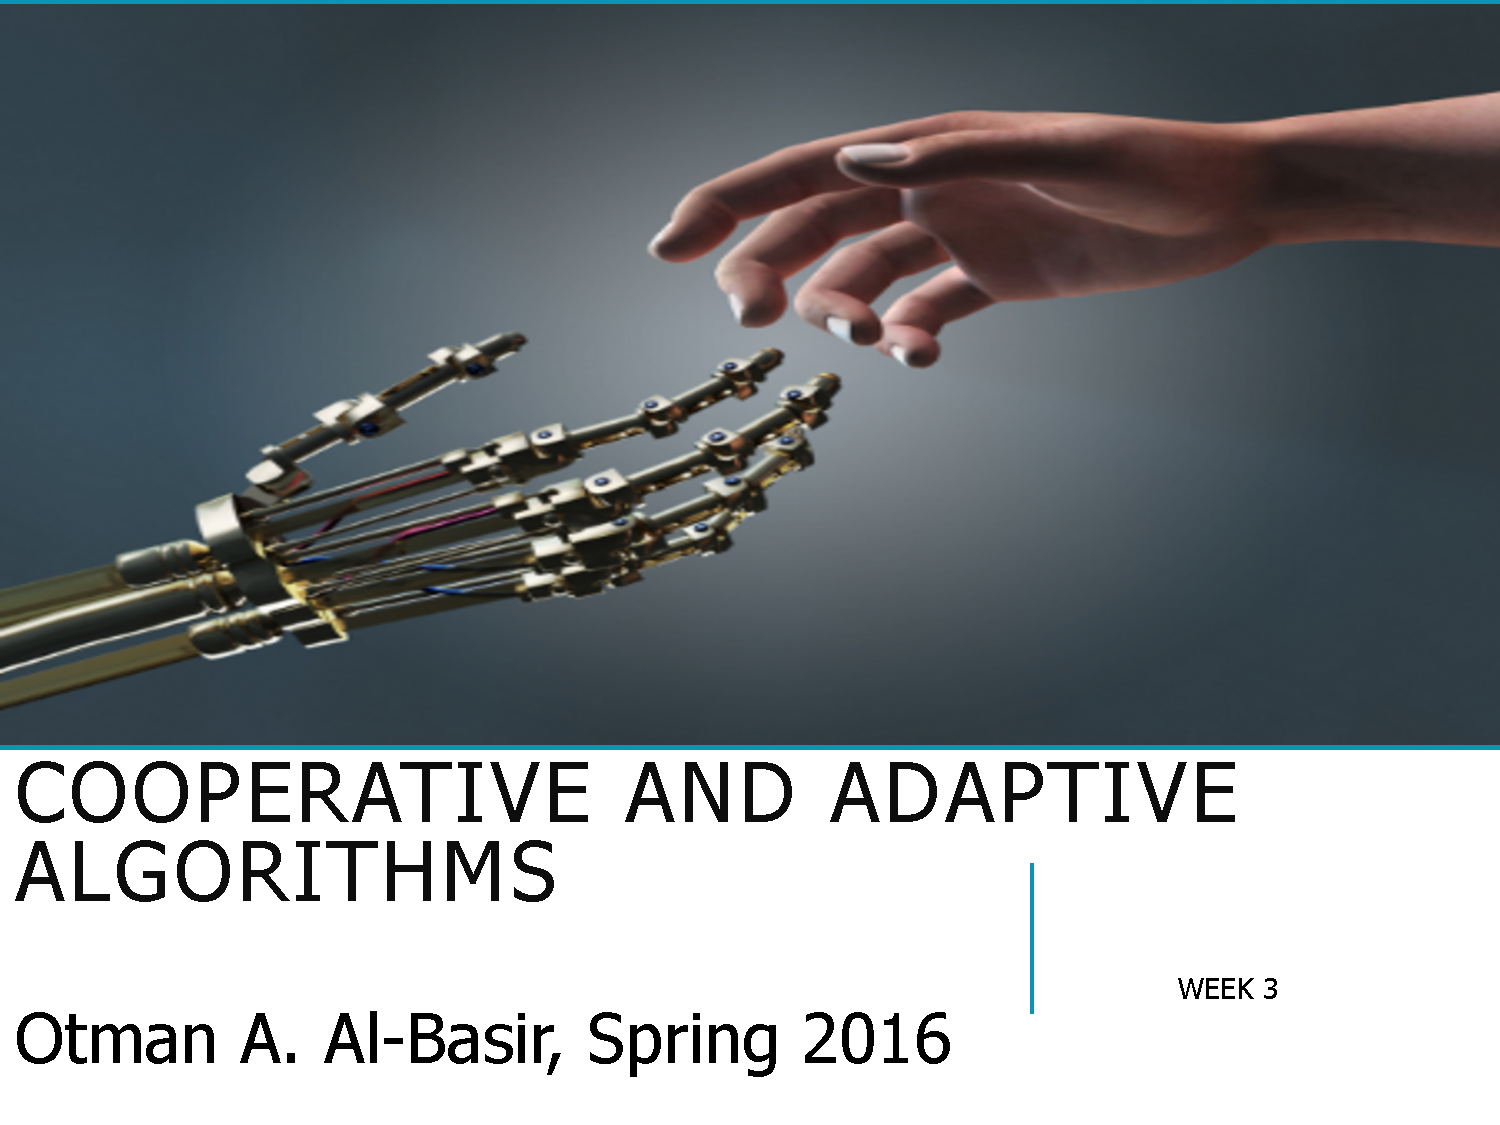
\includepdf[page=4-6]{slides.pdf}

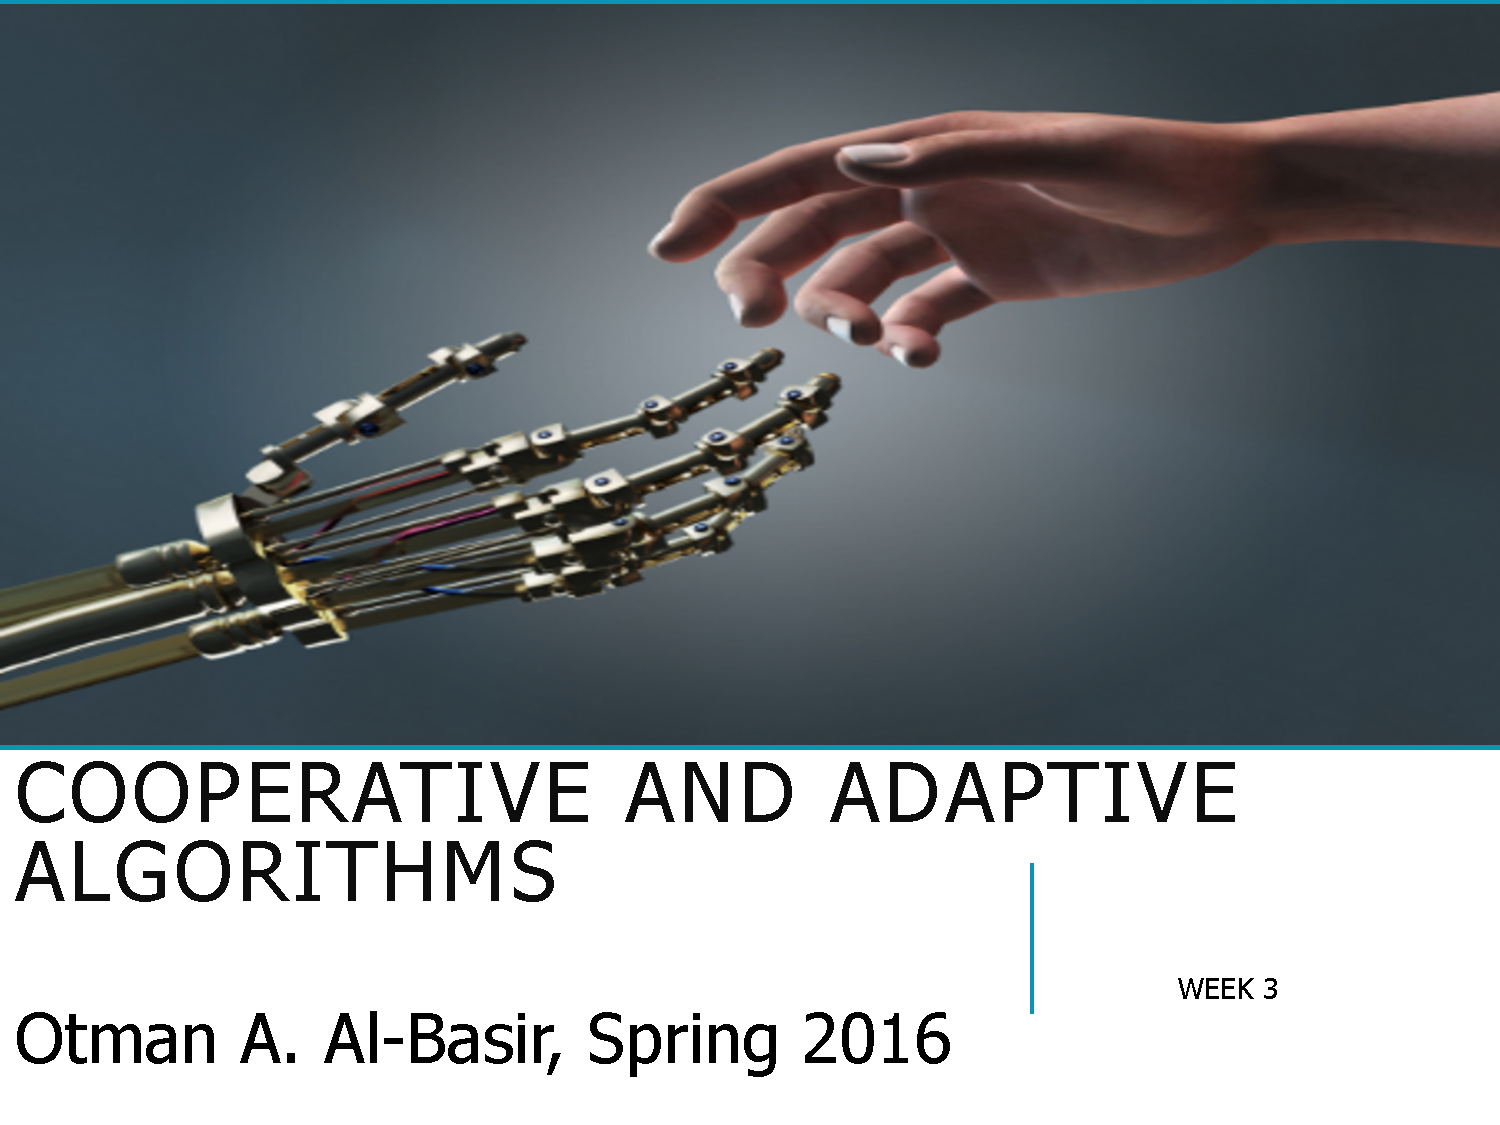
\includepdf[page=8-14]{slides.pdf}

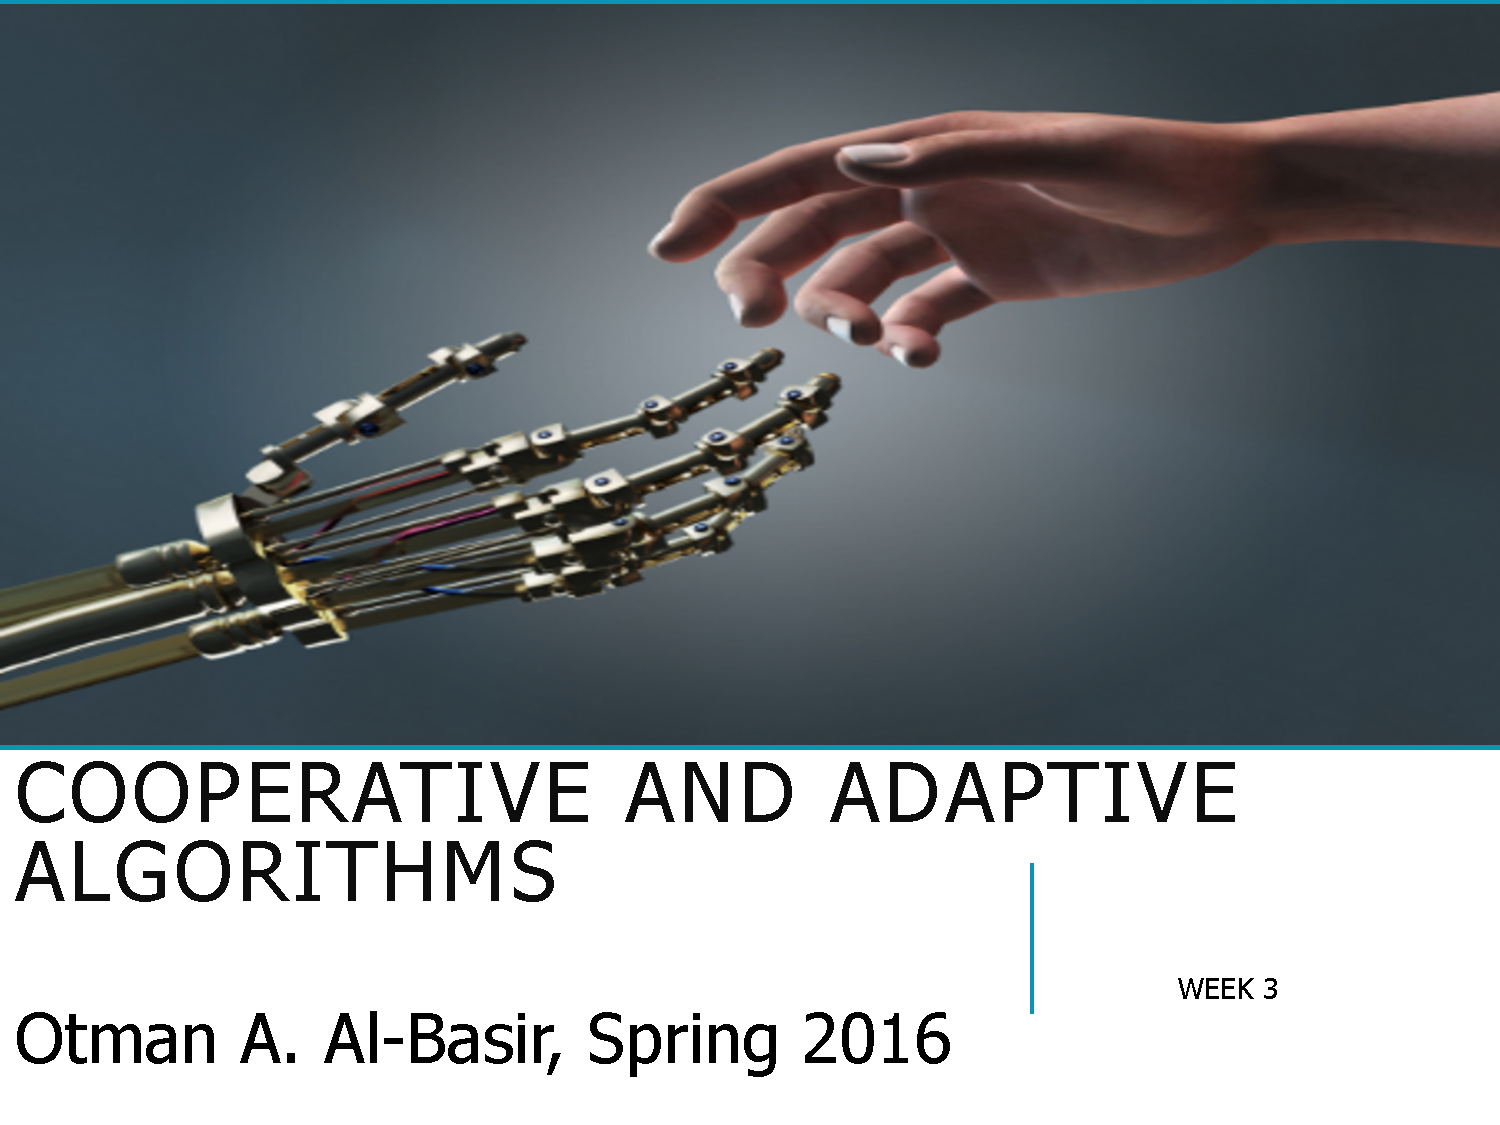
\includepdf[page=16-19]{slides.pdf}

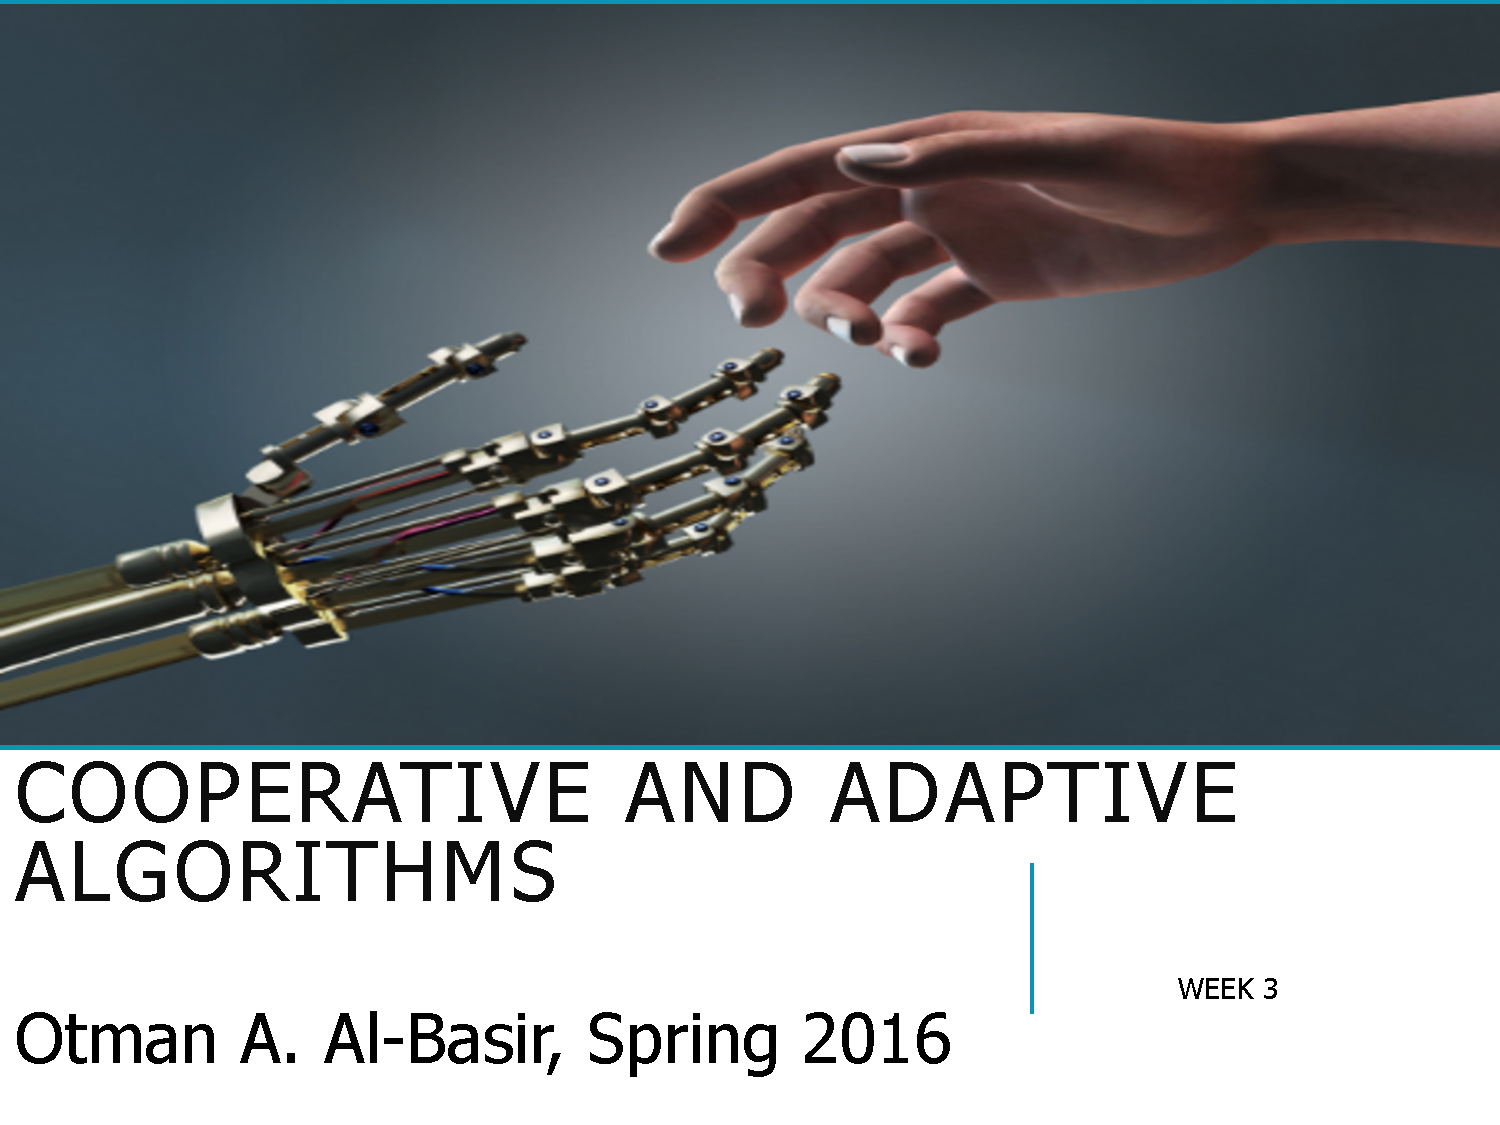
\includepdf[page=20]{slides.pdf}
We store the state in a circle and we connect it with a line that describes the event trigger and action taken to get to the next state. 

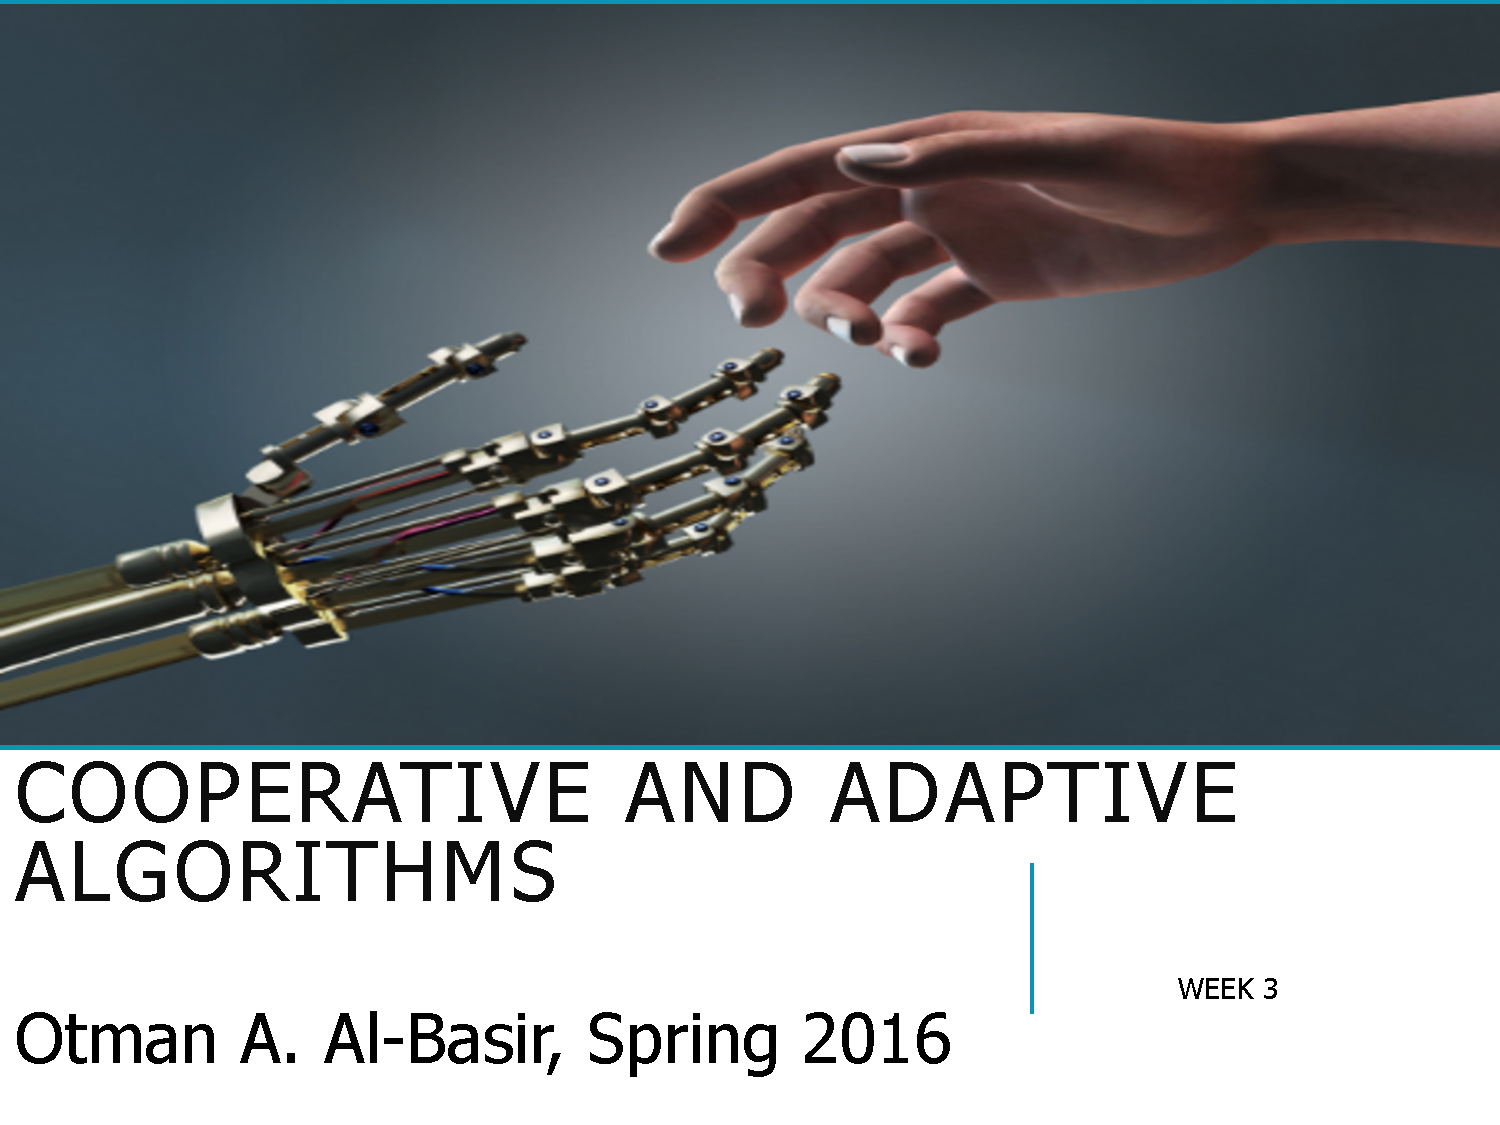
\includepdf[page=21]{slides.pdf}
We want to assume that we have no errors or loss packets (this is totally not true, esspecially in a5). Then you just have to build a packet and call send. When receiving we just have to accept and depackage.

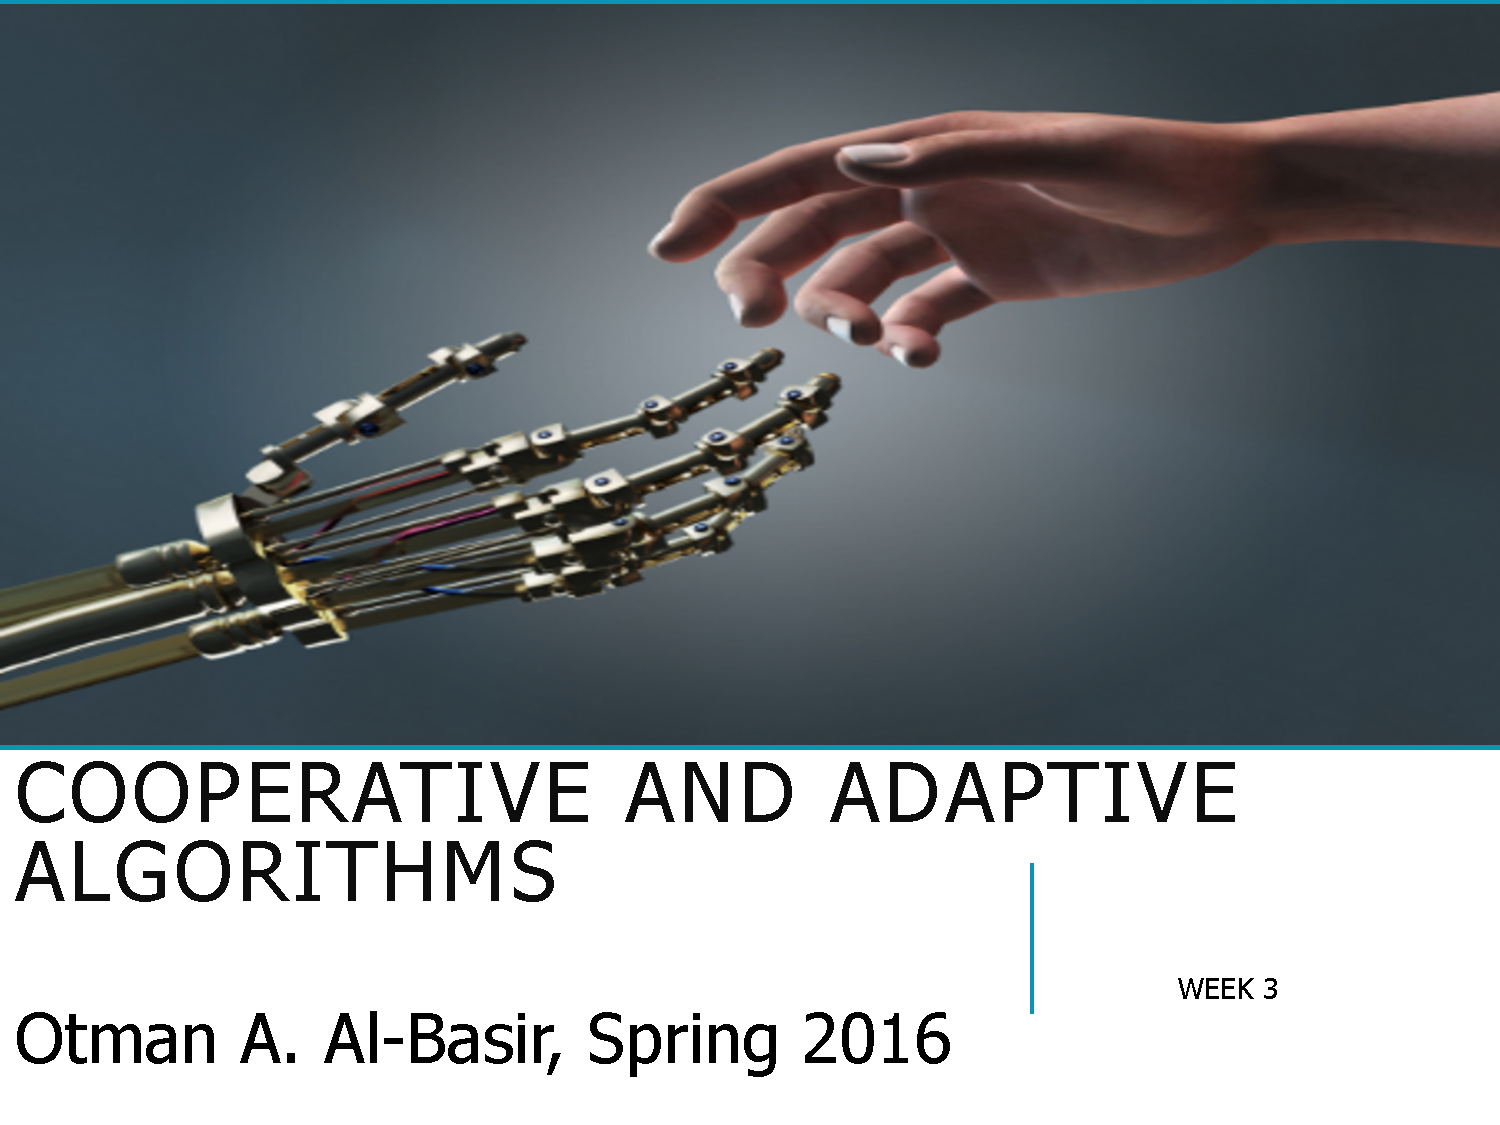
\includepdf[page=22]{slides.pdf}
What if we had errors? We need to assume that the receiver detects errors (don't try to correct errors, just notice them). 

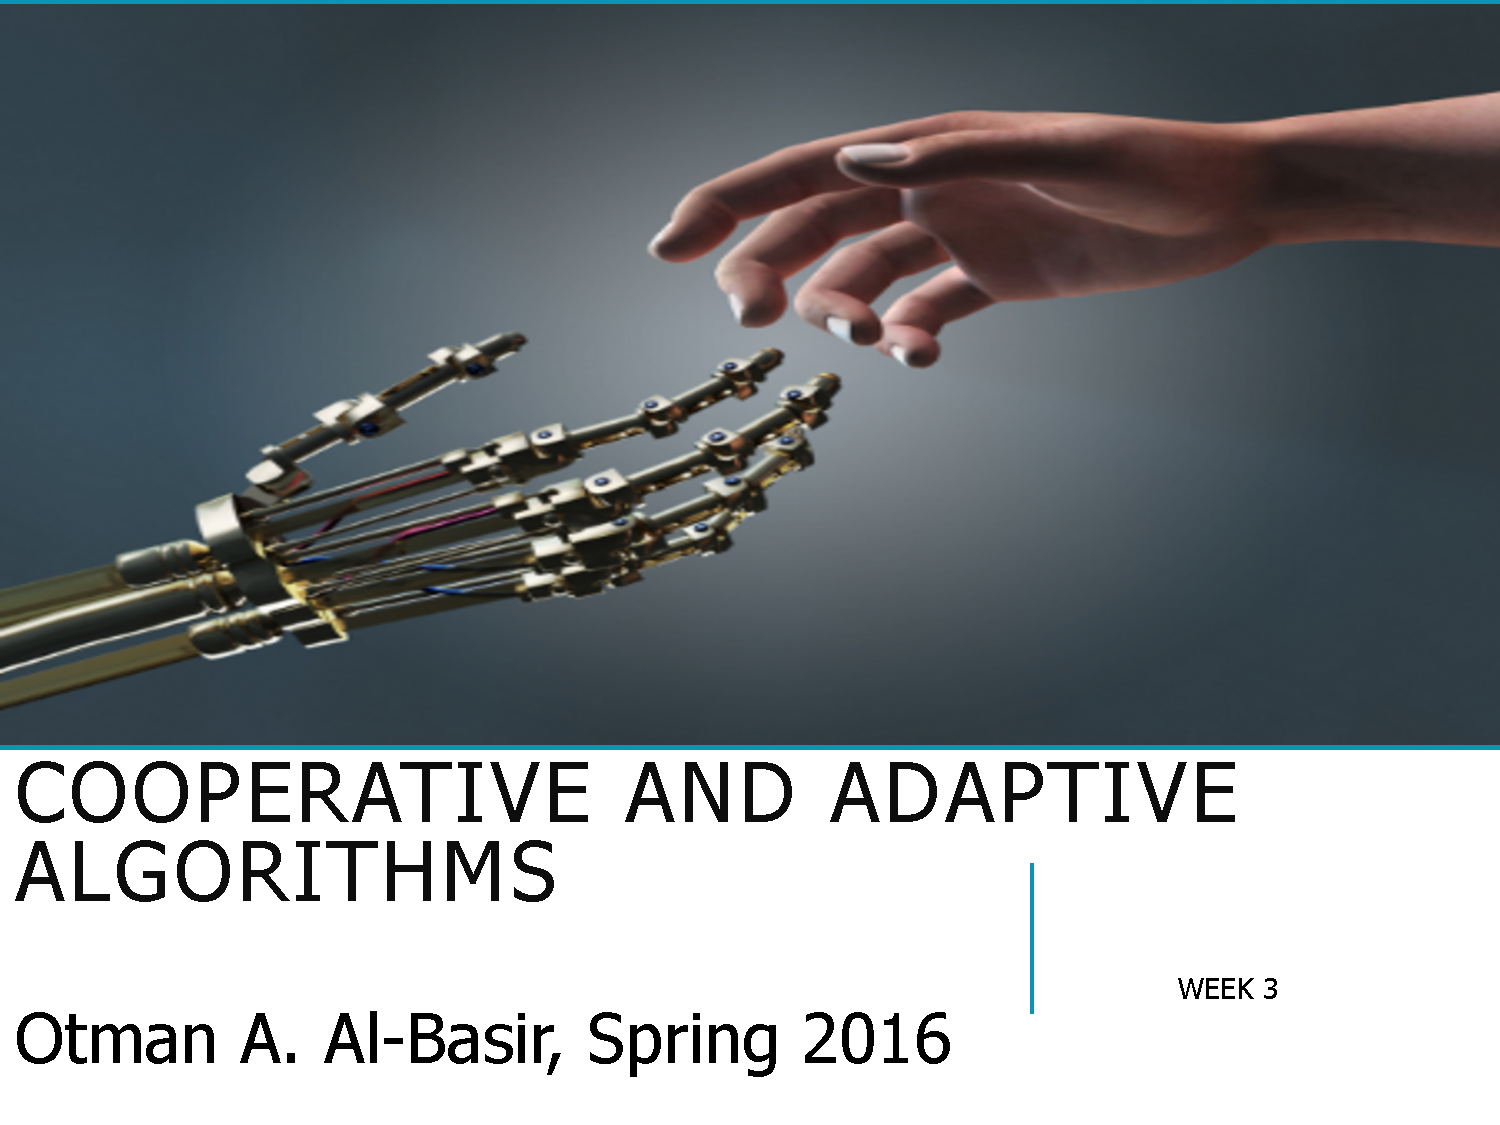
\includepdf[page=23]{slides.pdf}
Positive feedback is as acknowledgment sent as an ACK, basically responding that shit went through ok. A negative feedback, NACK, should trigger a resend.

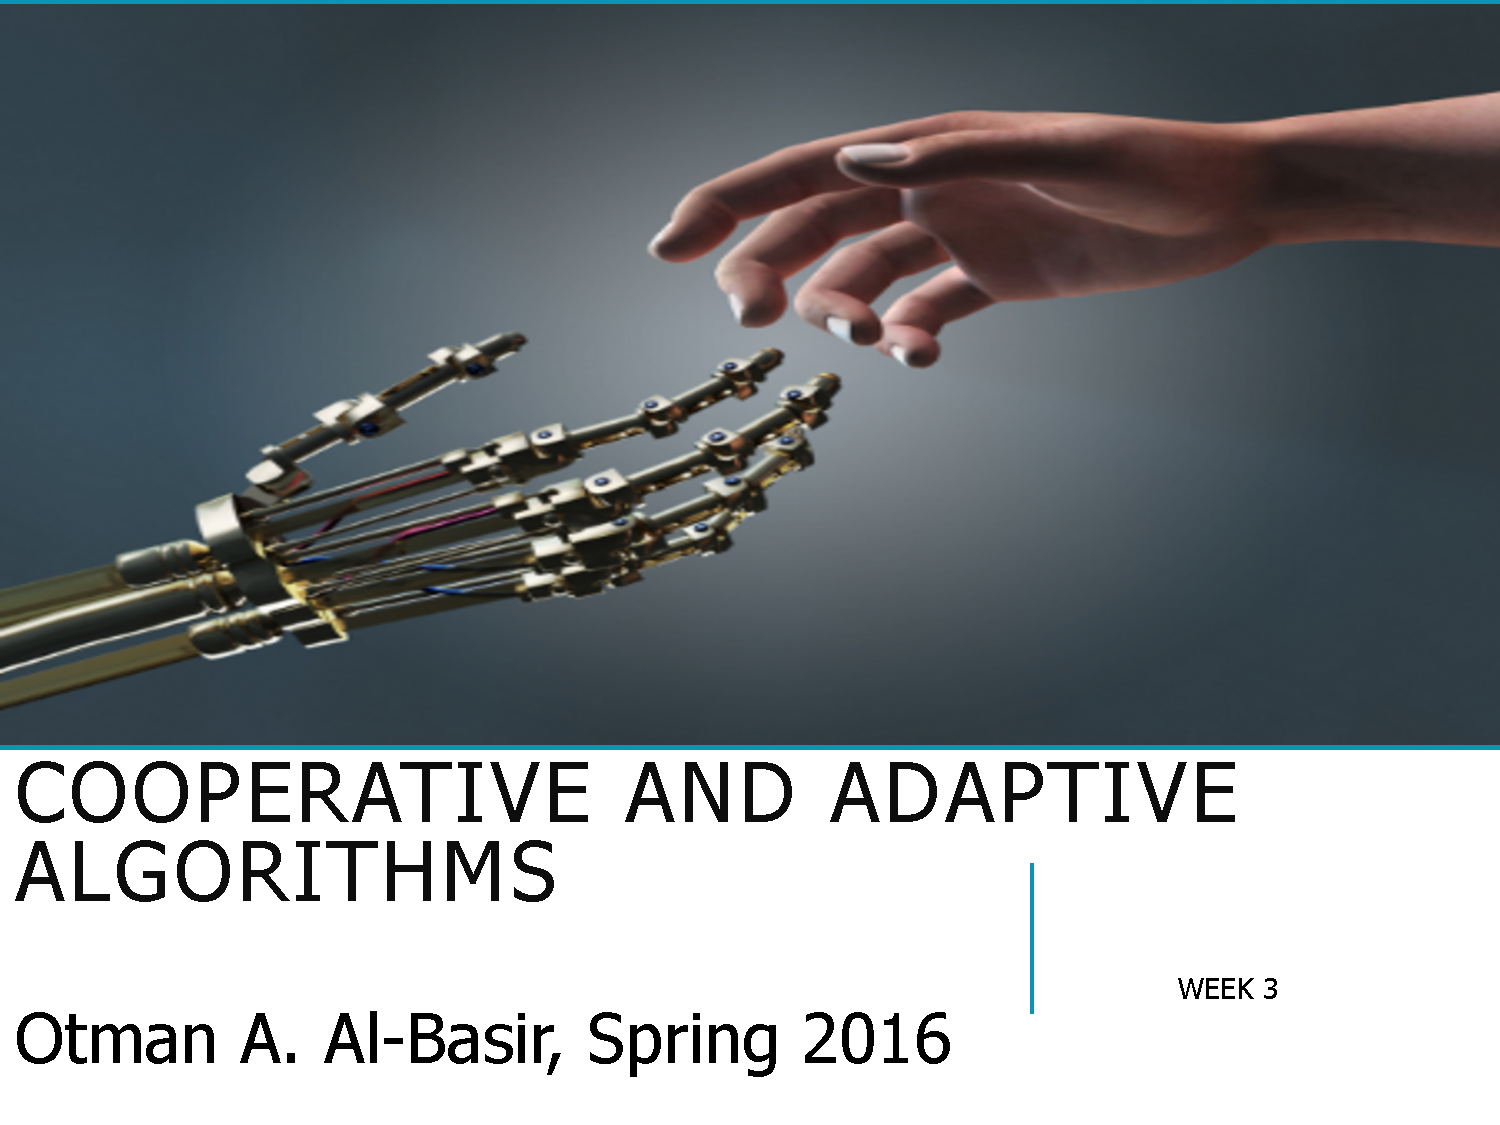
\includepdf[page=24]{slides.pdf}
rdt\_send = Make a packet, send using unreliable send, wait on rdt\_receive, check for negative ACK, is so resend, else got back to first state.

Important to note that the send is blocked until a receive happens

rdt\_receive = accept packet, check for errors (checksum), if so send NACK, else extract it and send ACK.


This procedure seems simple but there is a problem, what happens if sending an ACK fails?

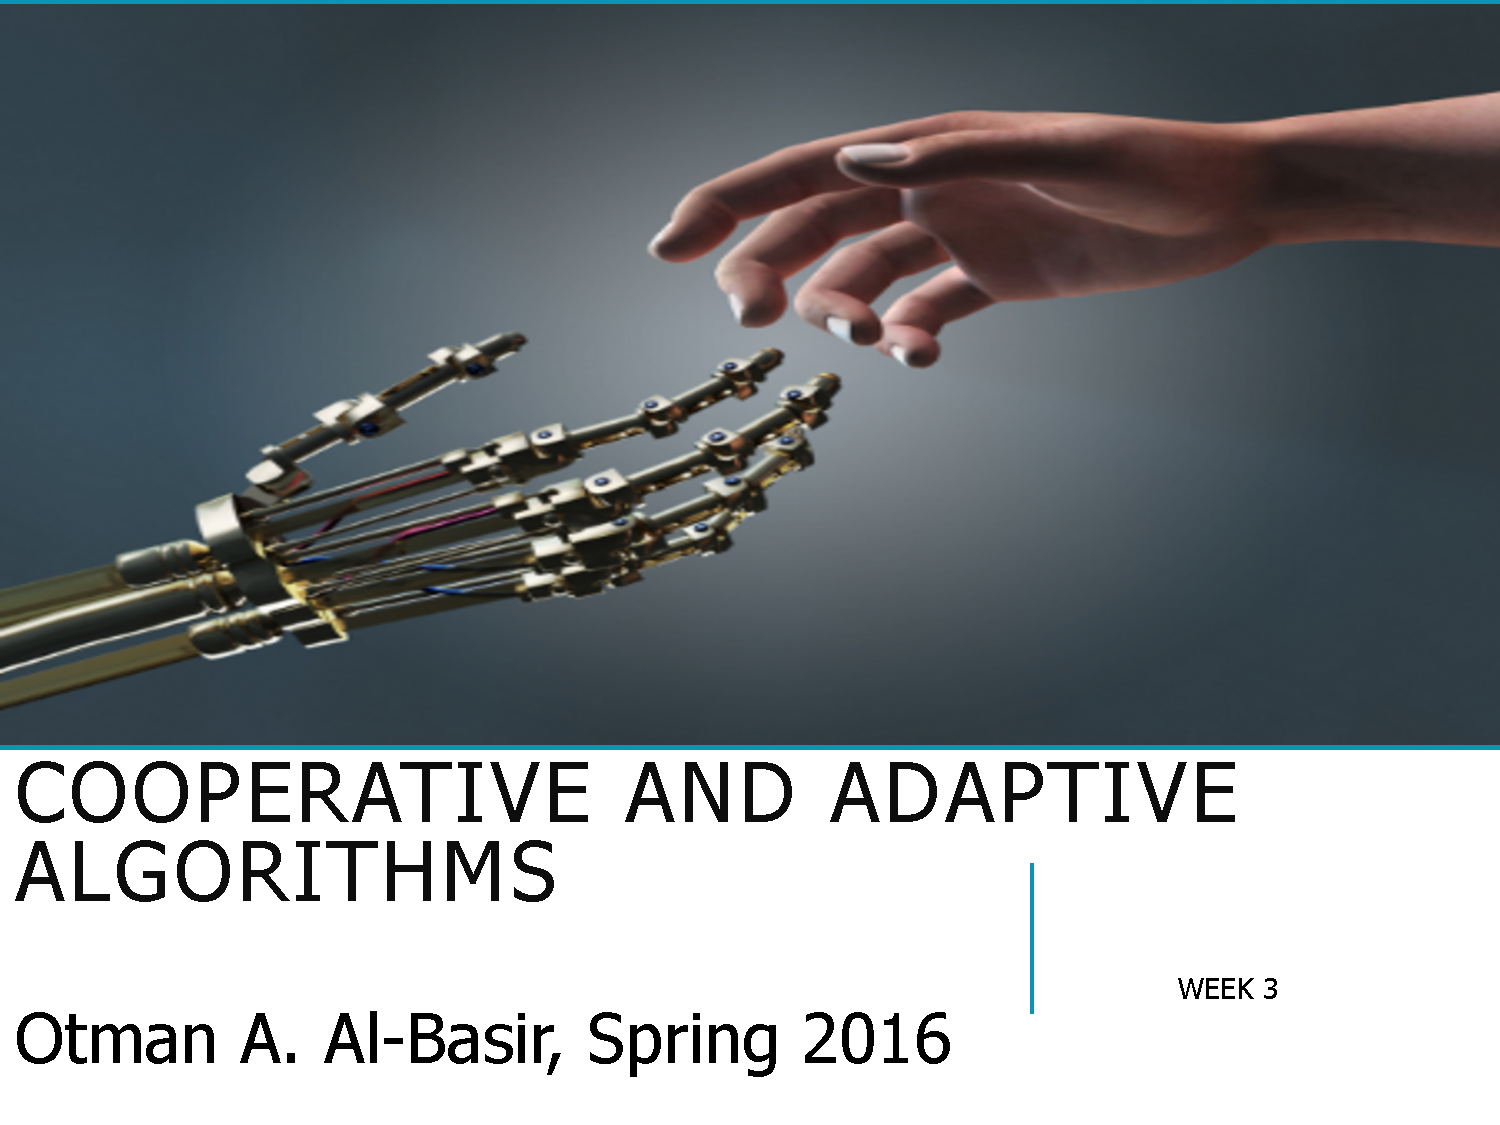
\includepdf[page=25-26]{slides.pdf}

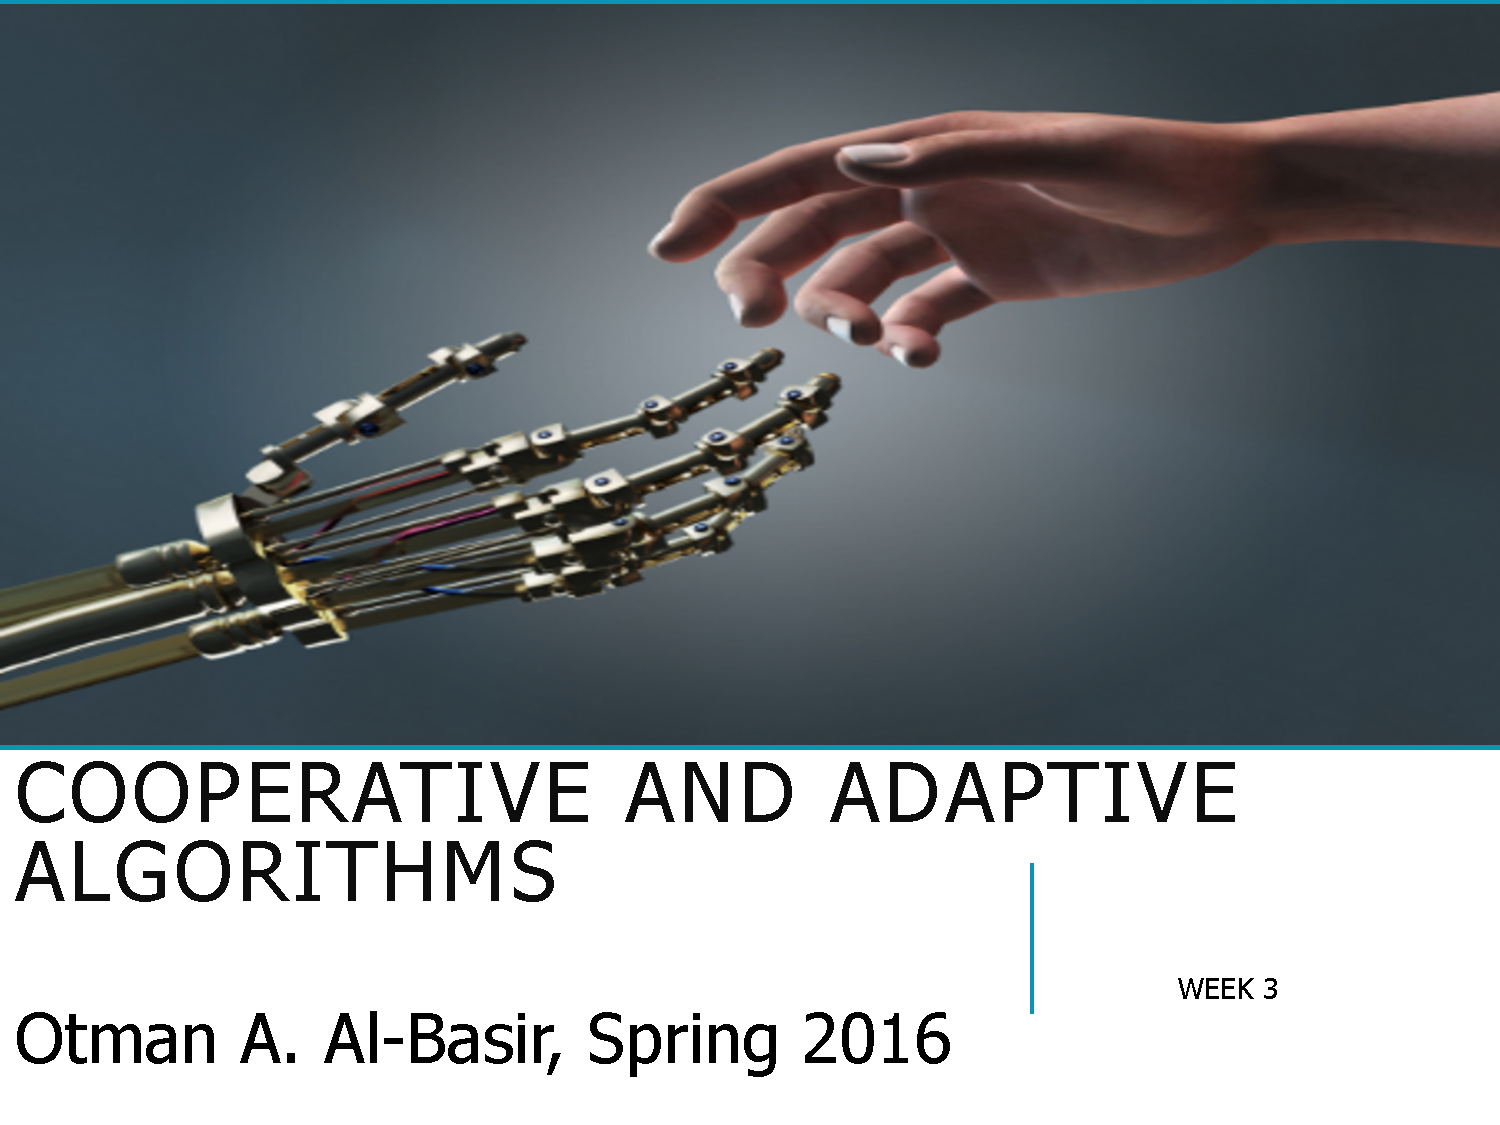
\includepdf[page=27]{slides.pdf}
We know that we've received a ACK or NACK, but that it is corrupted. We can't just ask the application to resend because we might be sending duplicate data which is unacceptable. So we incorporate  sequence number. We resend the packet including this sequence number. The client now has a whole bunch of protocols around handling that number. The simplest one is called stop and wait. The sender sends a packet and waits until a good acknowledgement comes through.

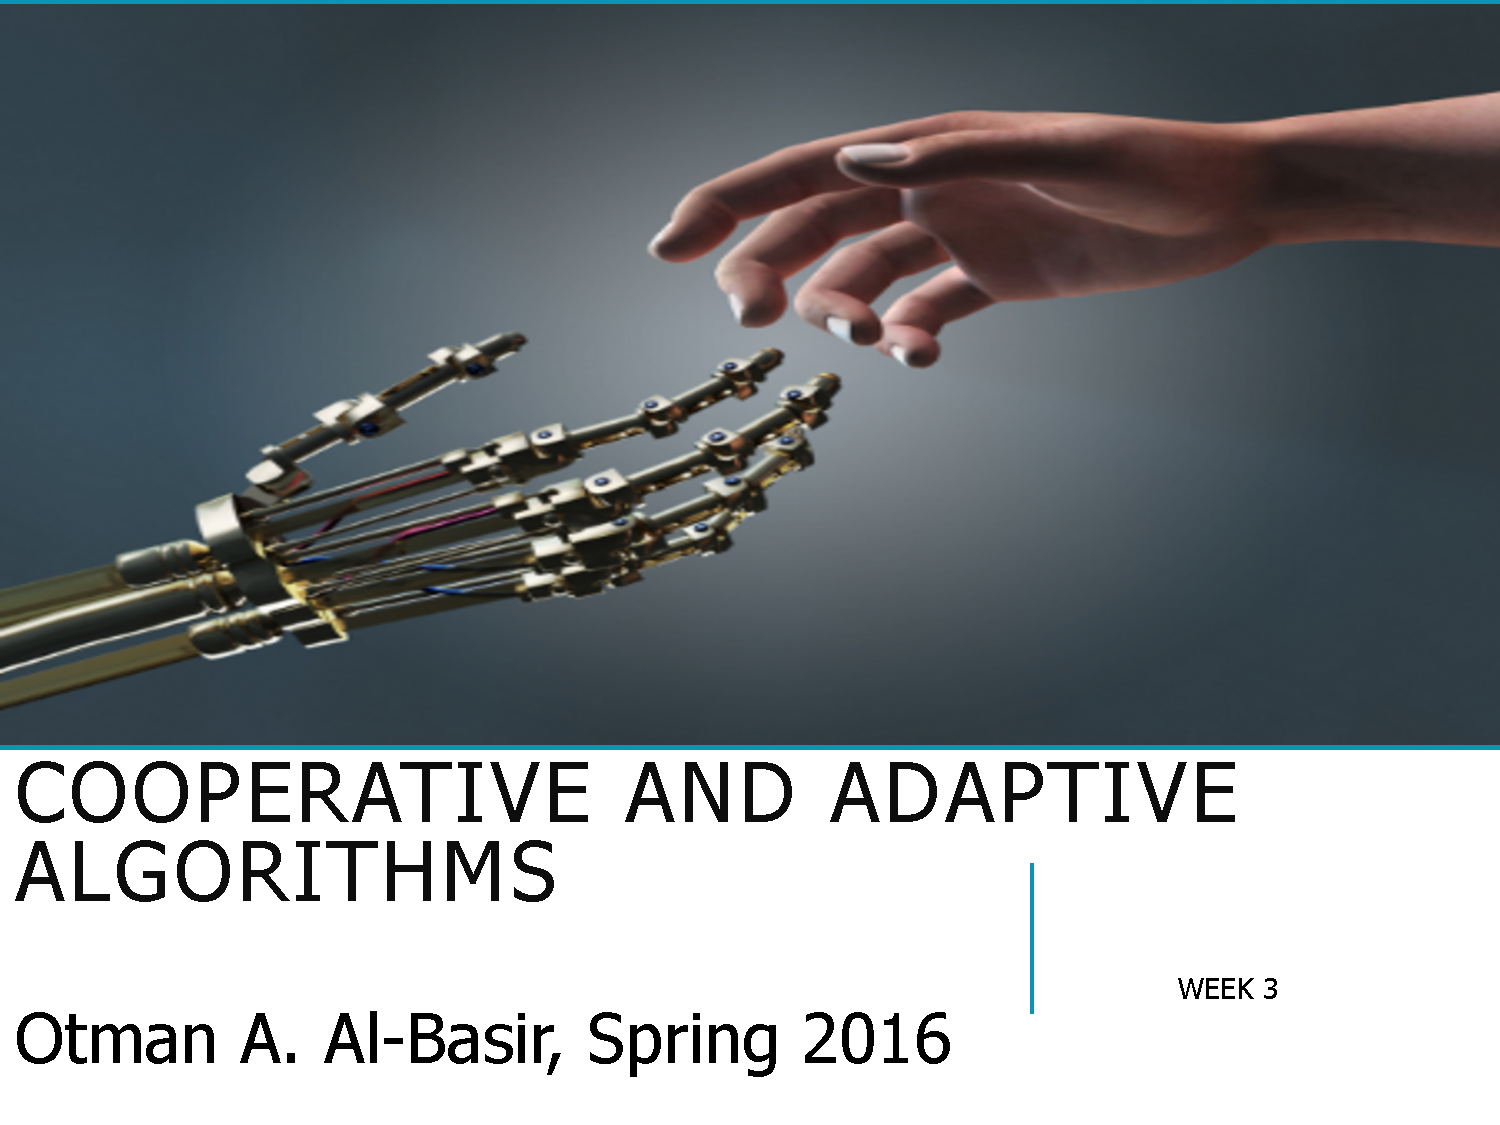
\includepdf[page=28]{slides.pdf}
Create a packet with the sequence 0, wait for ACK. If we receive a corrupted one or a NACK we resend the packet with the same sequence, else we increment our sequence and continue forward. 


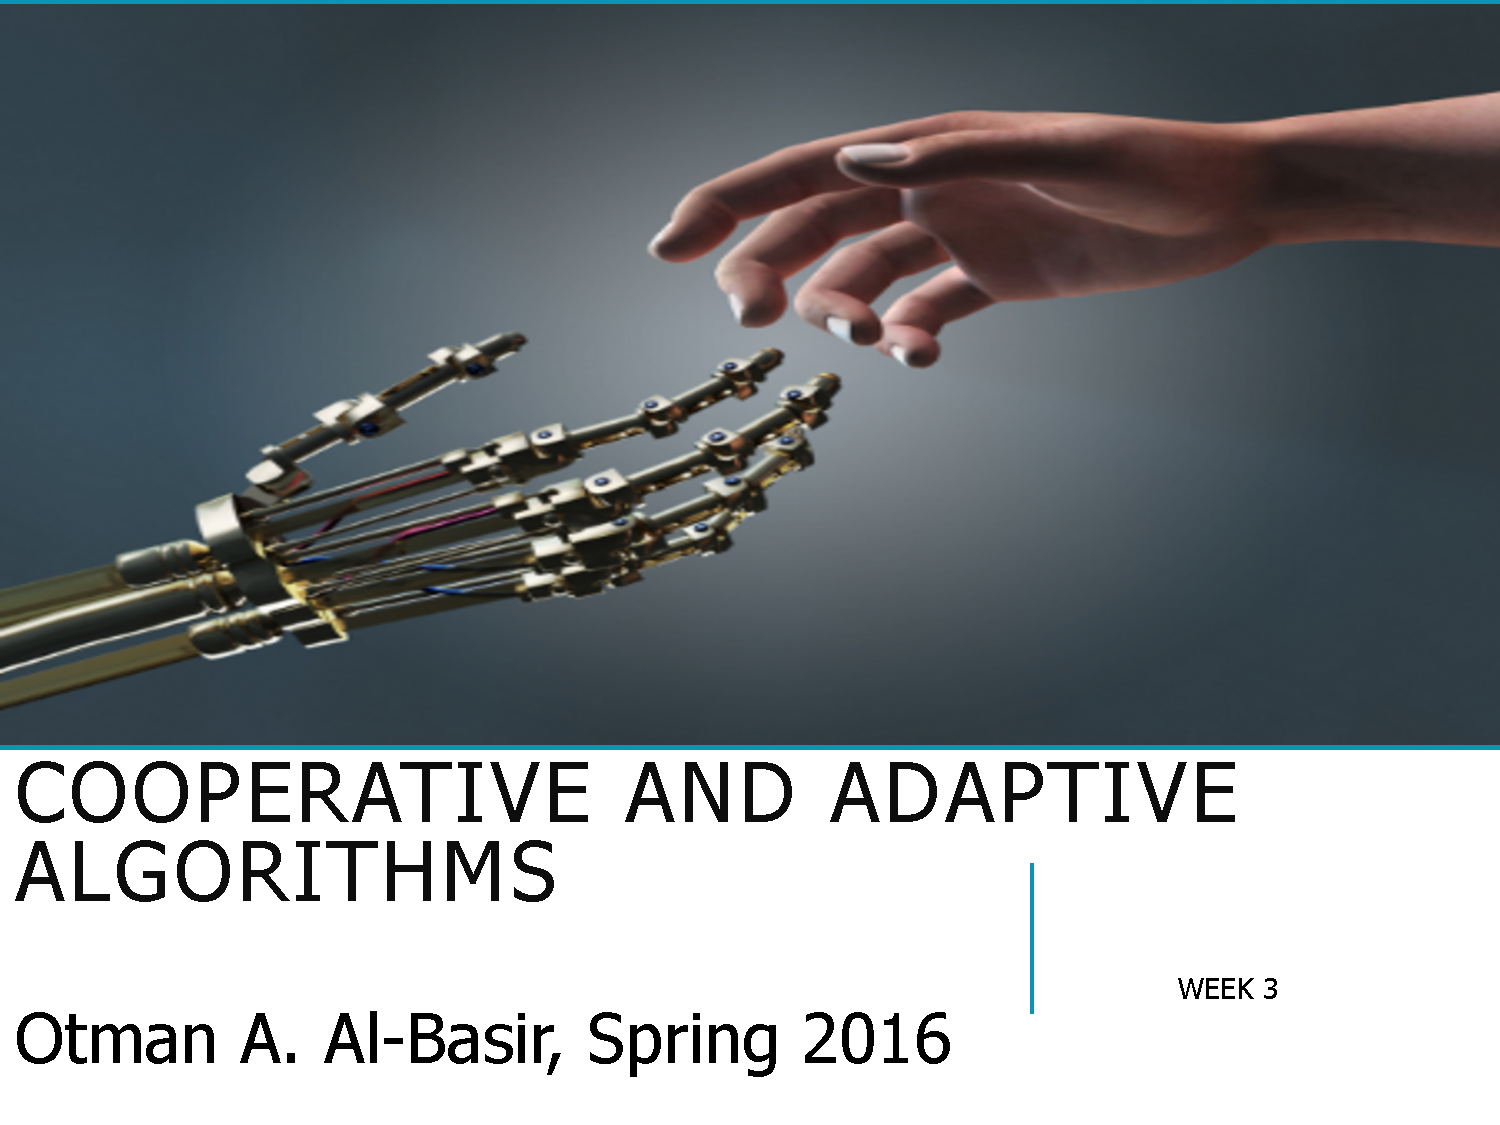
\includepdf[page=29]{slides.pdf}
When we receive a packet we need to check both the checksum and the sequence number before extracting it. Then we increment our sequence number. If we receive a perfectly good packet with the wrong sequence number then we have to assume that the other side received a packet that we didn't send which implies a packet loss which we are assuming didn't happen. 

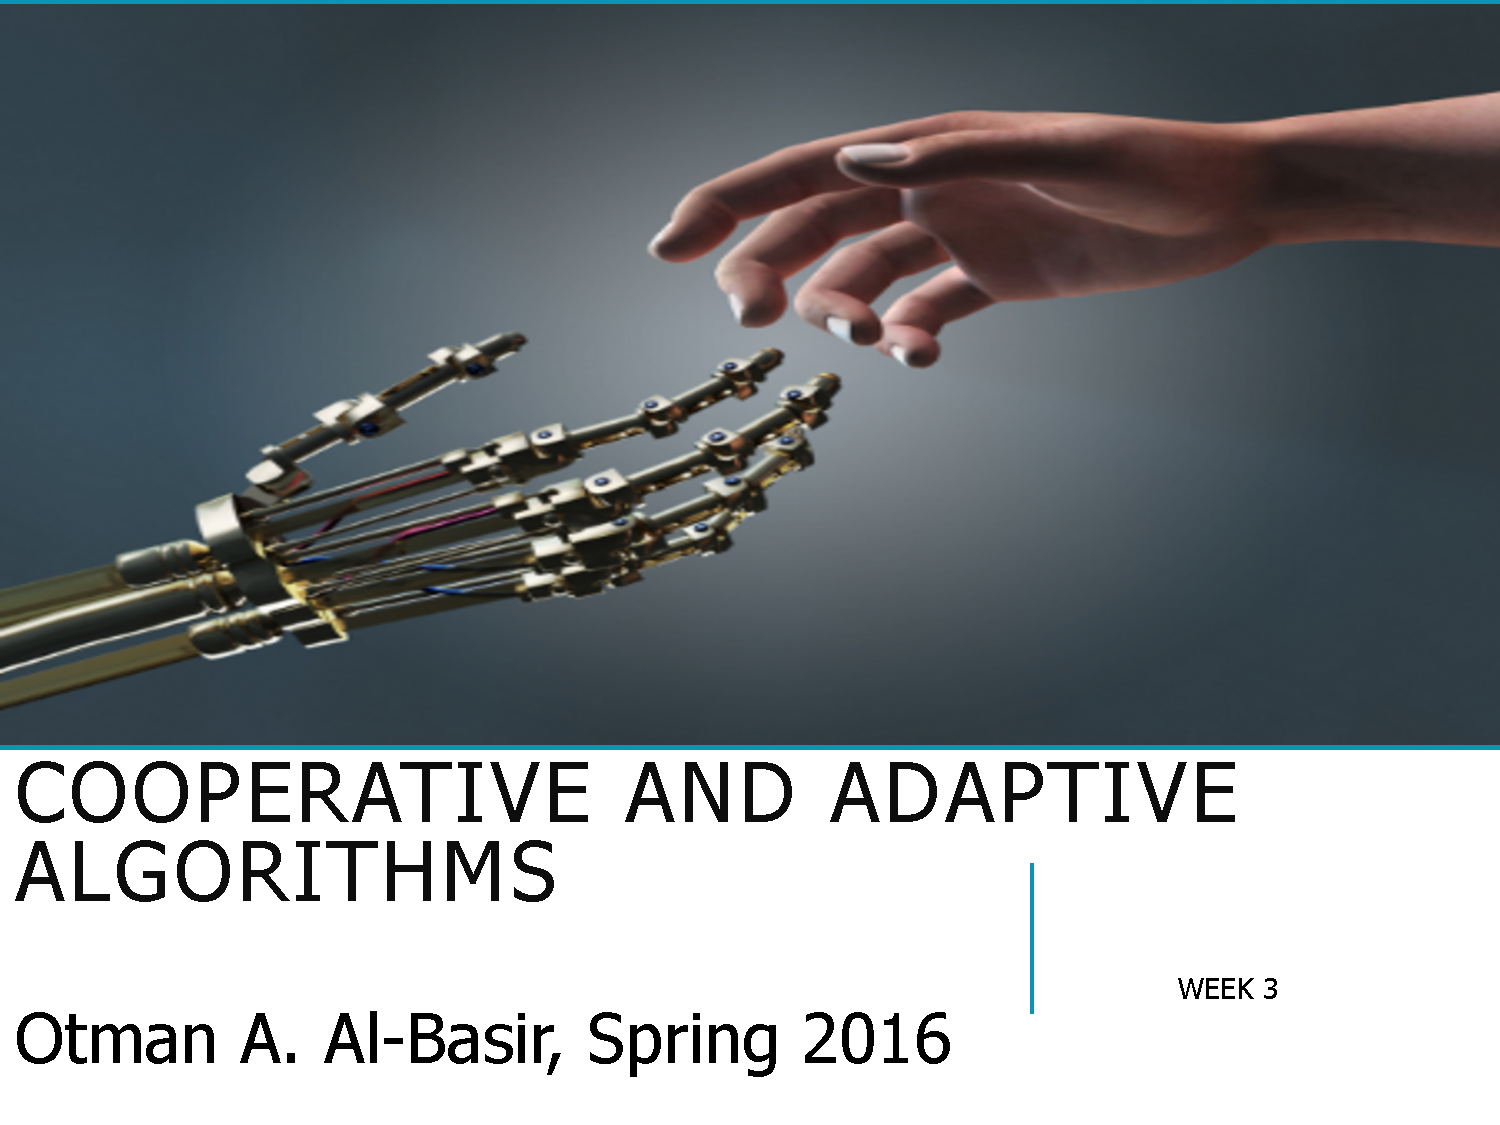
\includepdf[page=30]{slides.pdf}
You can get infinite loops if the channel keeps corrupting your data. TCP has a hack around this, but its hackey. Its teardown process is fairly complicated.

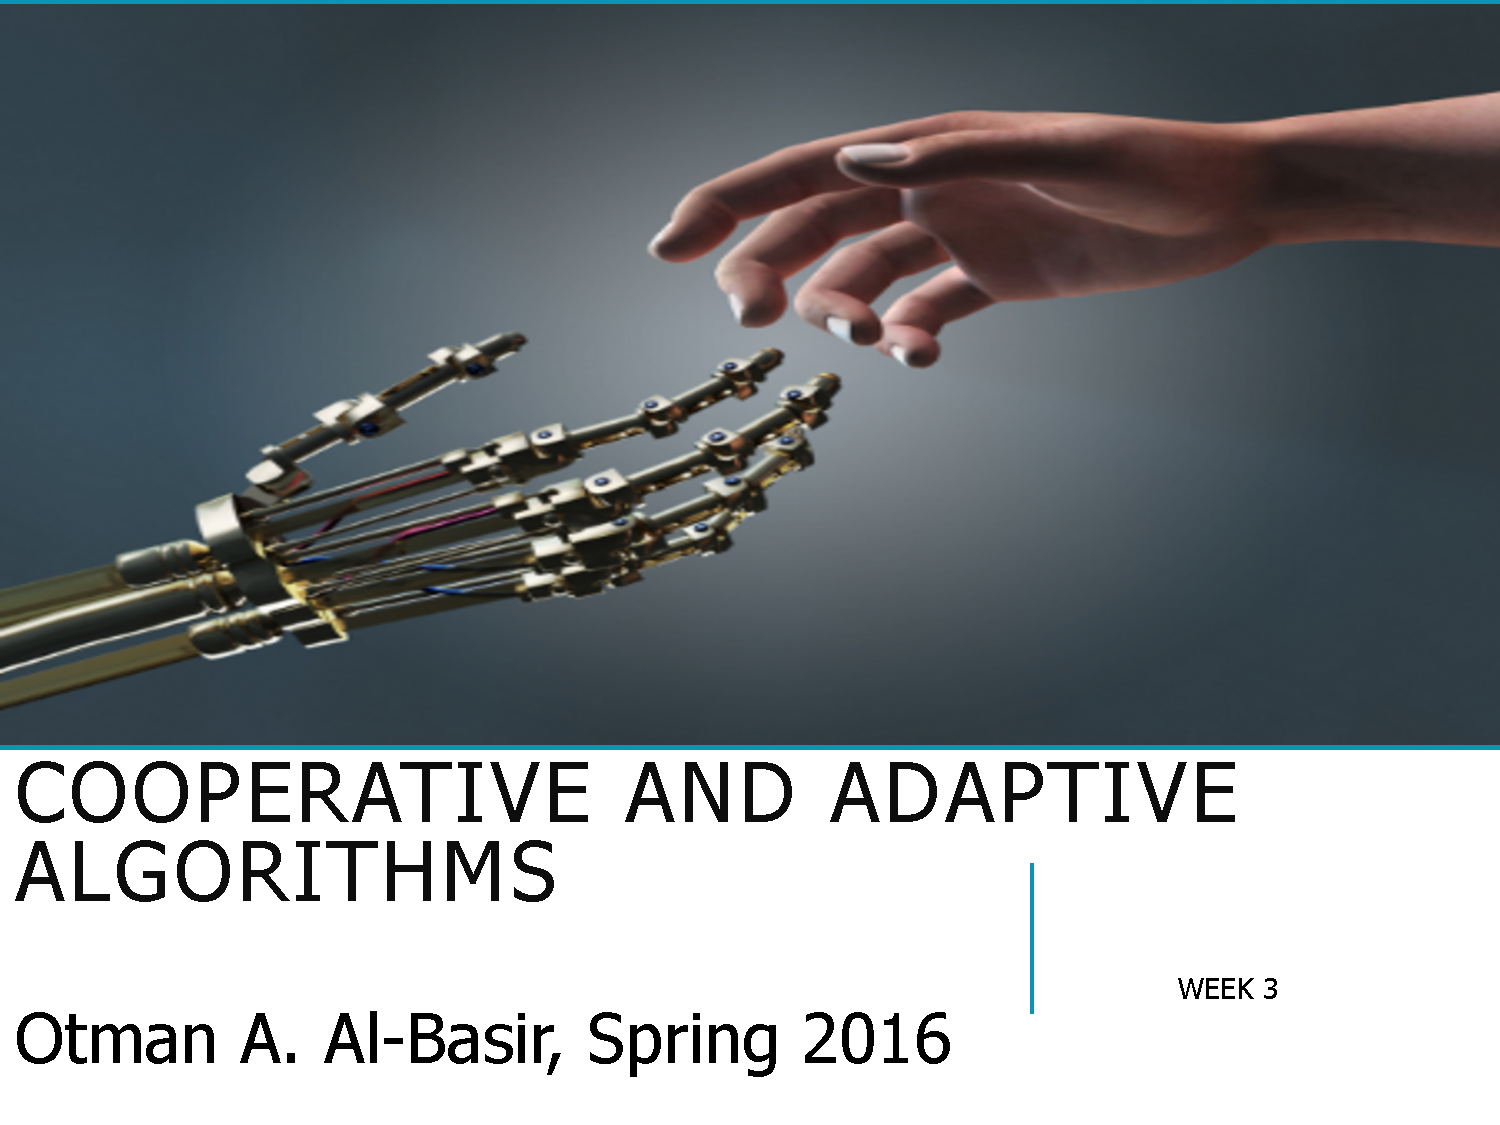
\includepdf[page=31]{slides.pdf}
We can make do with only one time of acknowledgement by making the sequence number in the ACK wrong.

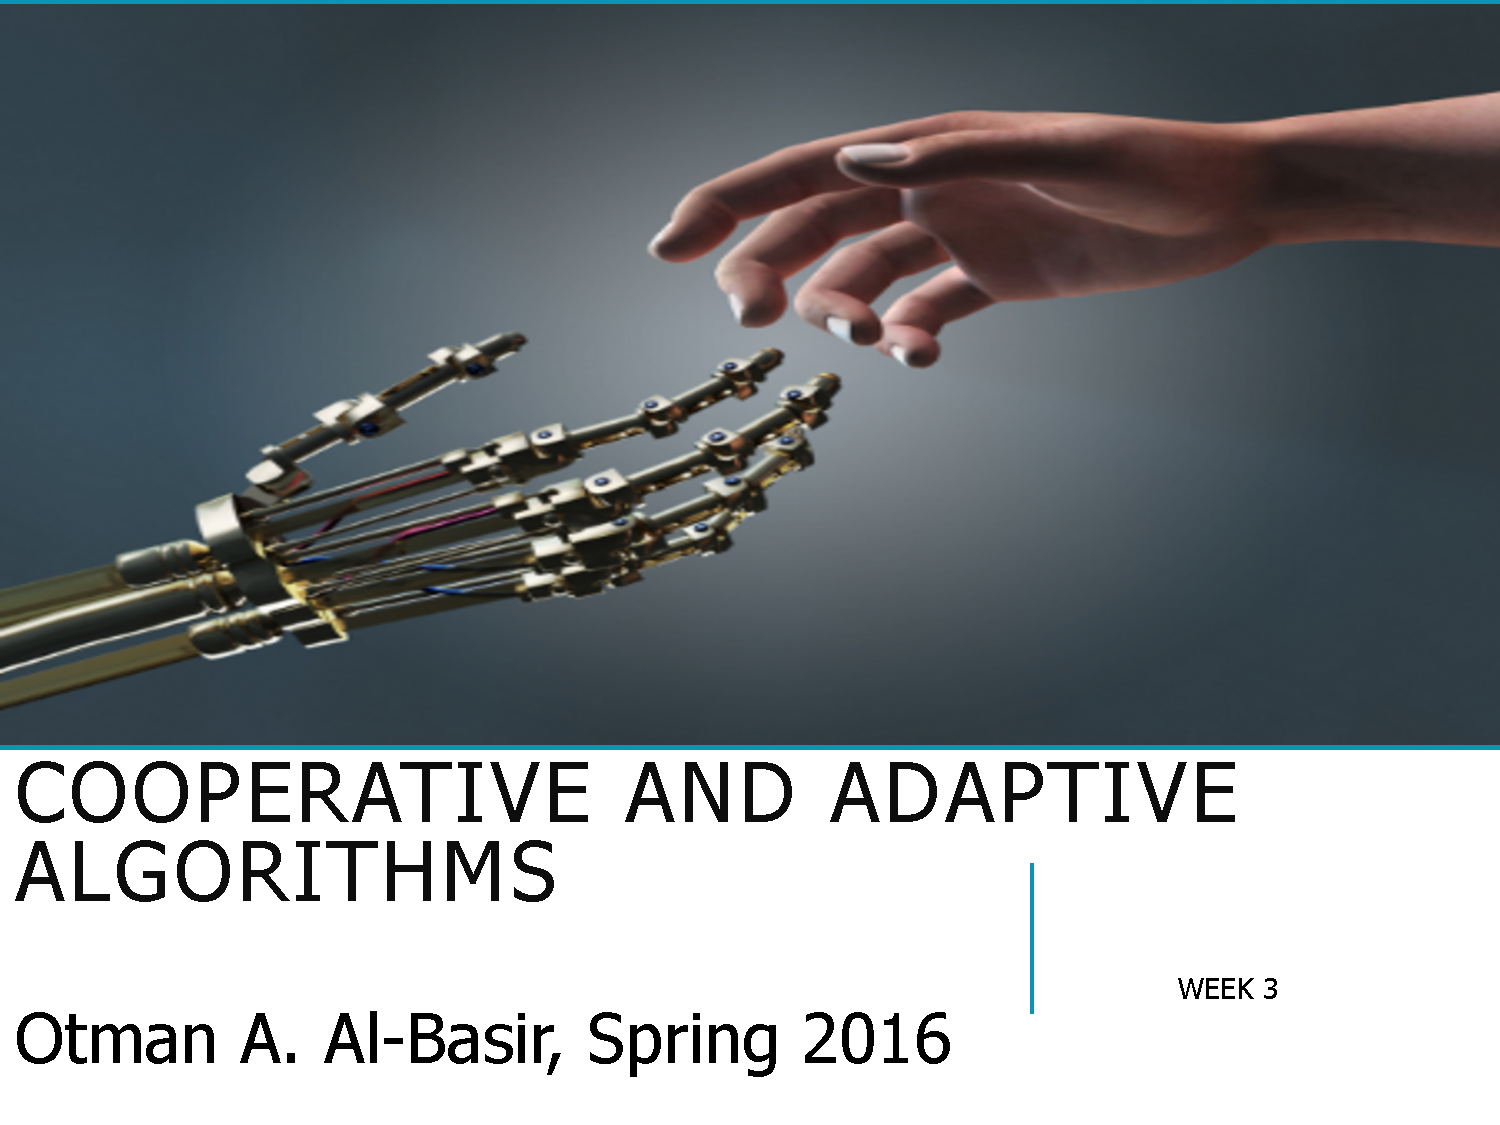
\includepdf[page=32]{slides.pdf}
Sending ACKs with wrong number can get a little finicky due to duplicate data being sent all over the place (for now we pretend that everything is blocking so you don't get concurency issues). The ways that TCP handles the sequence number is different from what these slides use. TCP has the sequence number say what number we expect to receive next and these slides say which number we just got.


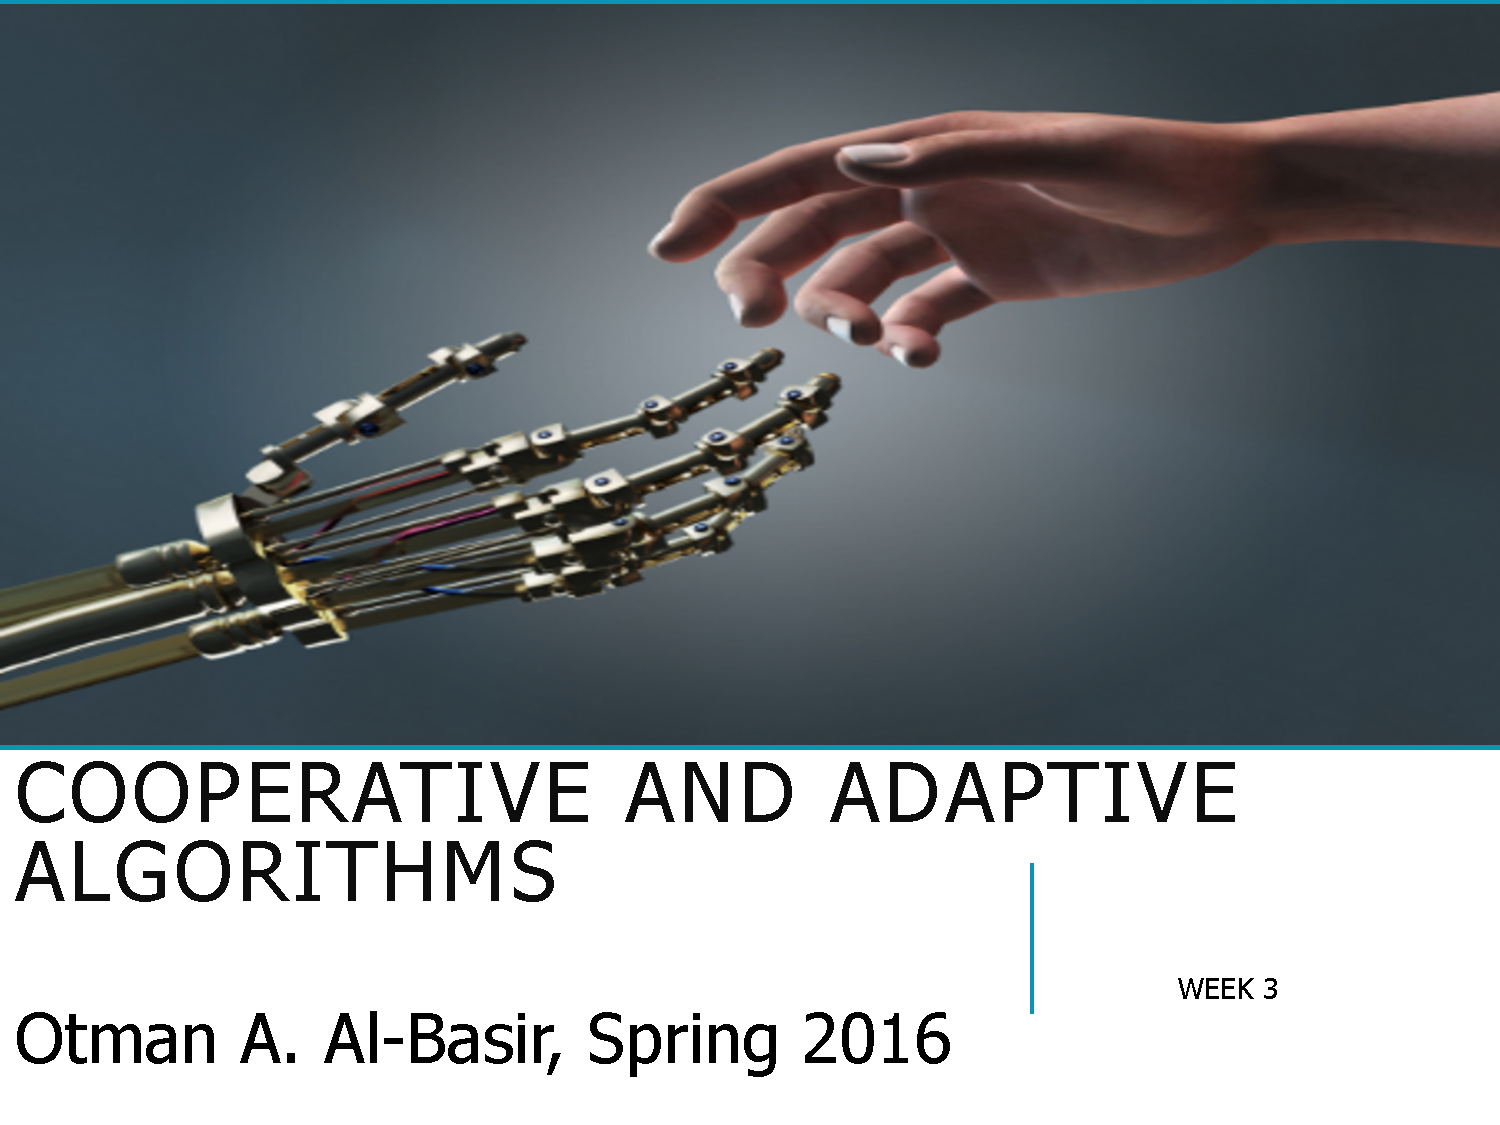
\includepdf[page=33]{slides.pdf}
Now we incorperate loss into our system. This is where timeouts are included.


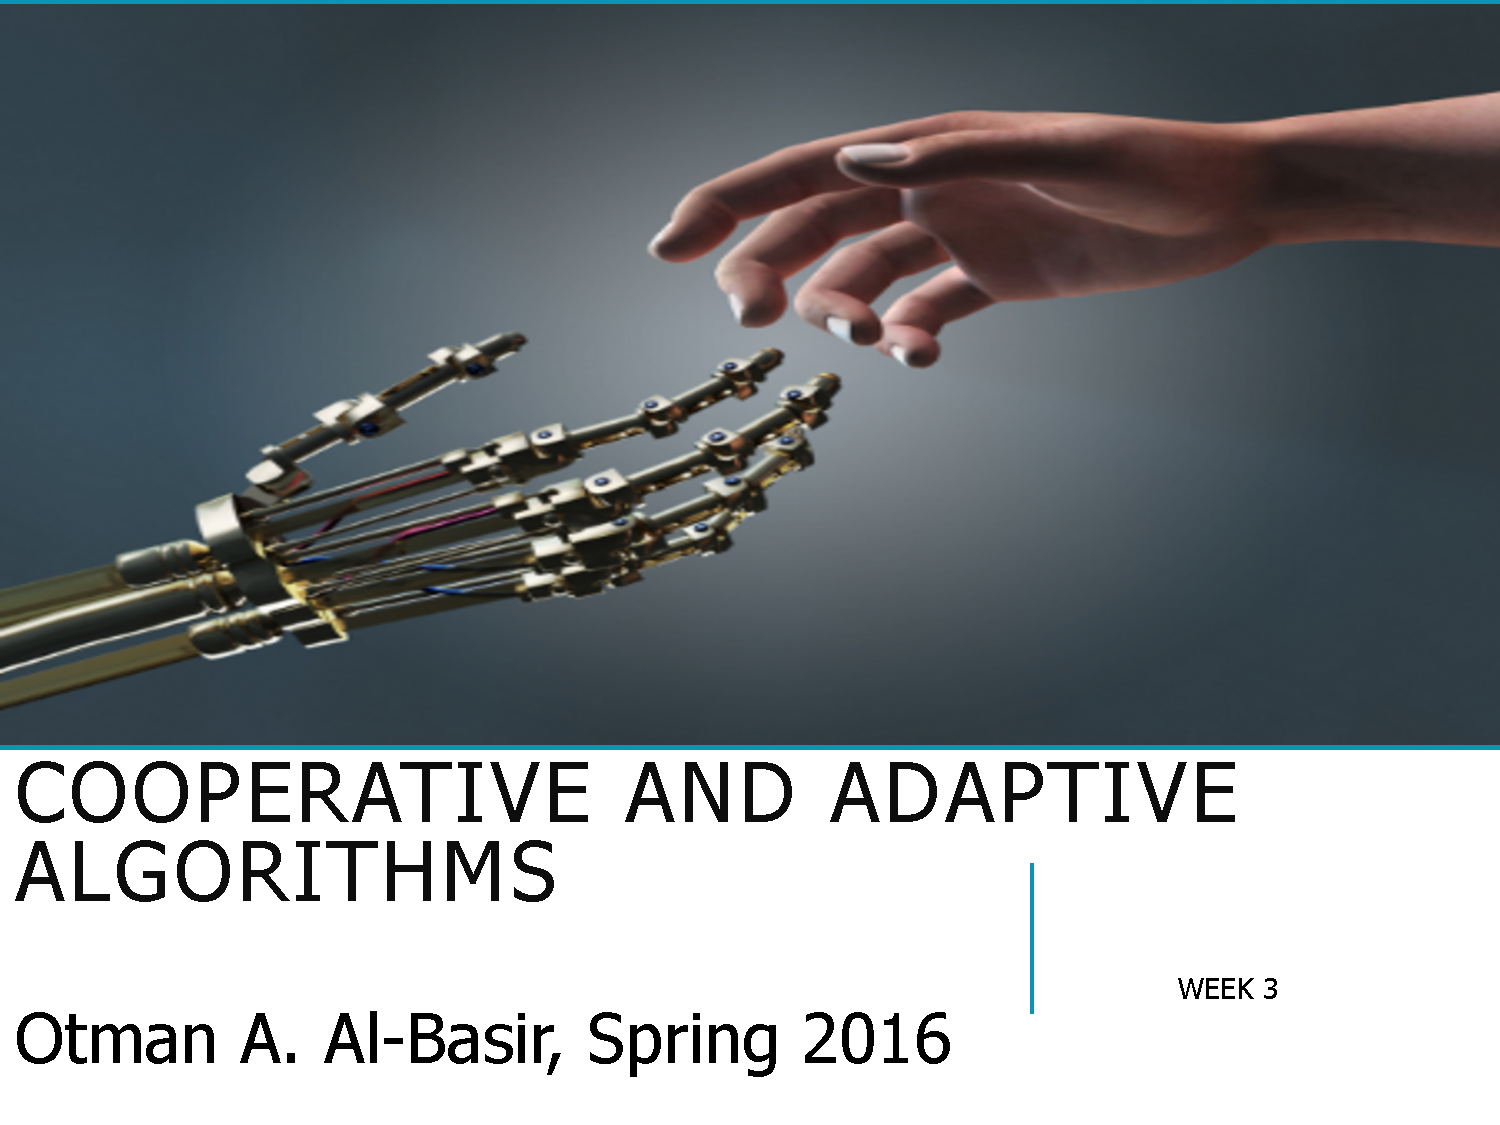
\includepdf[page=34]{slides.pdf}
The state for waiting for the ACK now has a timeout value that it checks against and will just resend if the timeout is reached. There might be duplicate packets, but we will have sequence numbers to handle it.

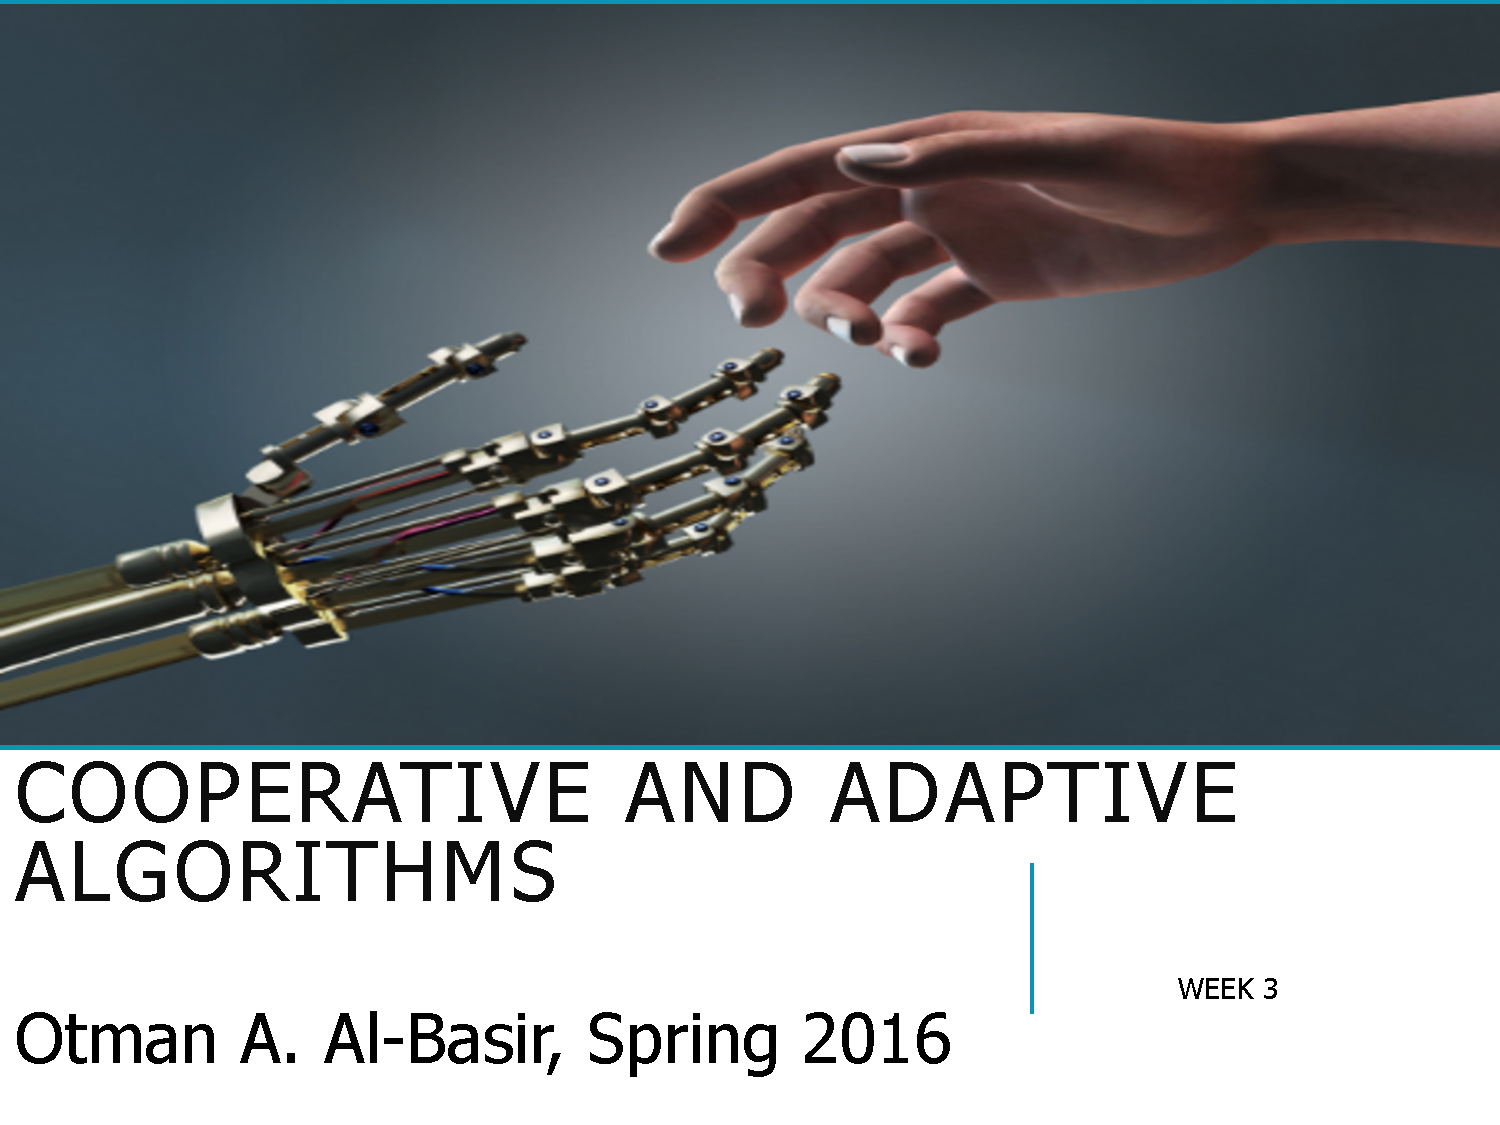
\includepdf[page=35]{slides.pdf}
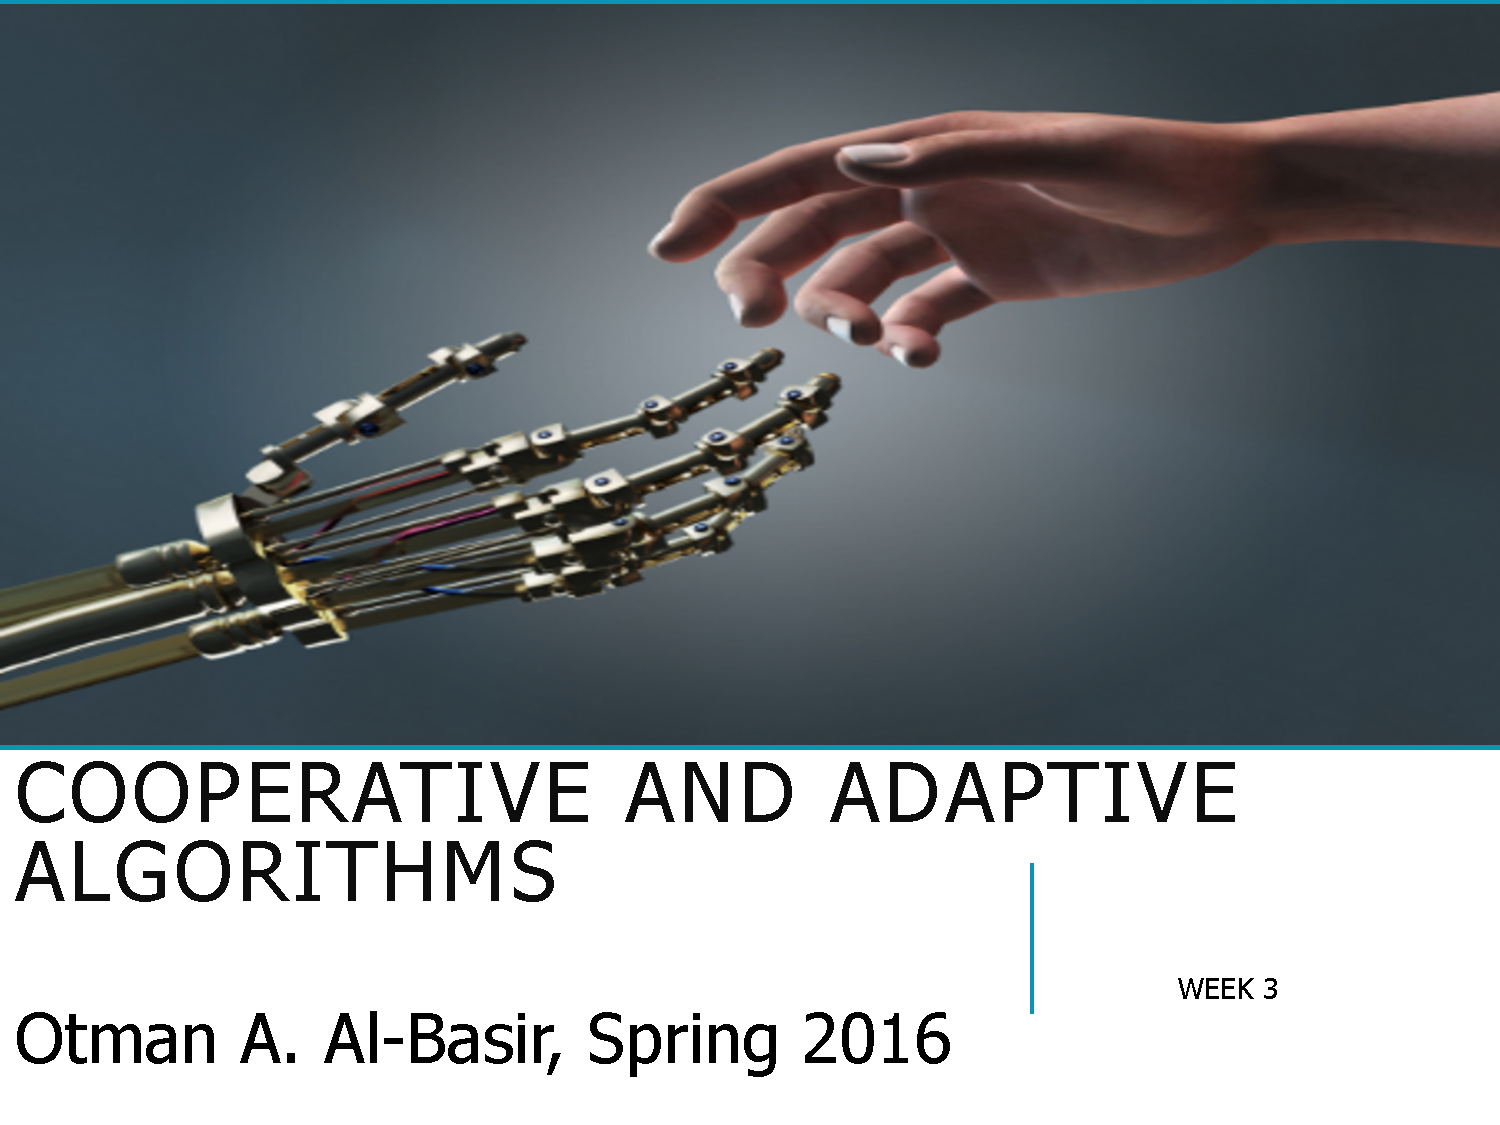
\includepdf[page=36]{slides.pdf}
Fuck I missed this.


THERE WILL BE A QUESTION ON THE ASSINGMENT ABOUT THE BUG IN THESE SLIDES BASED ON THE STATEMACHINE

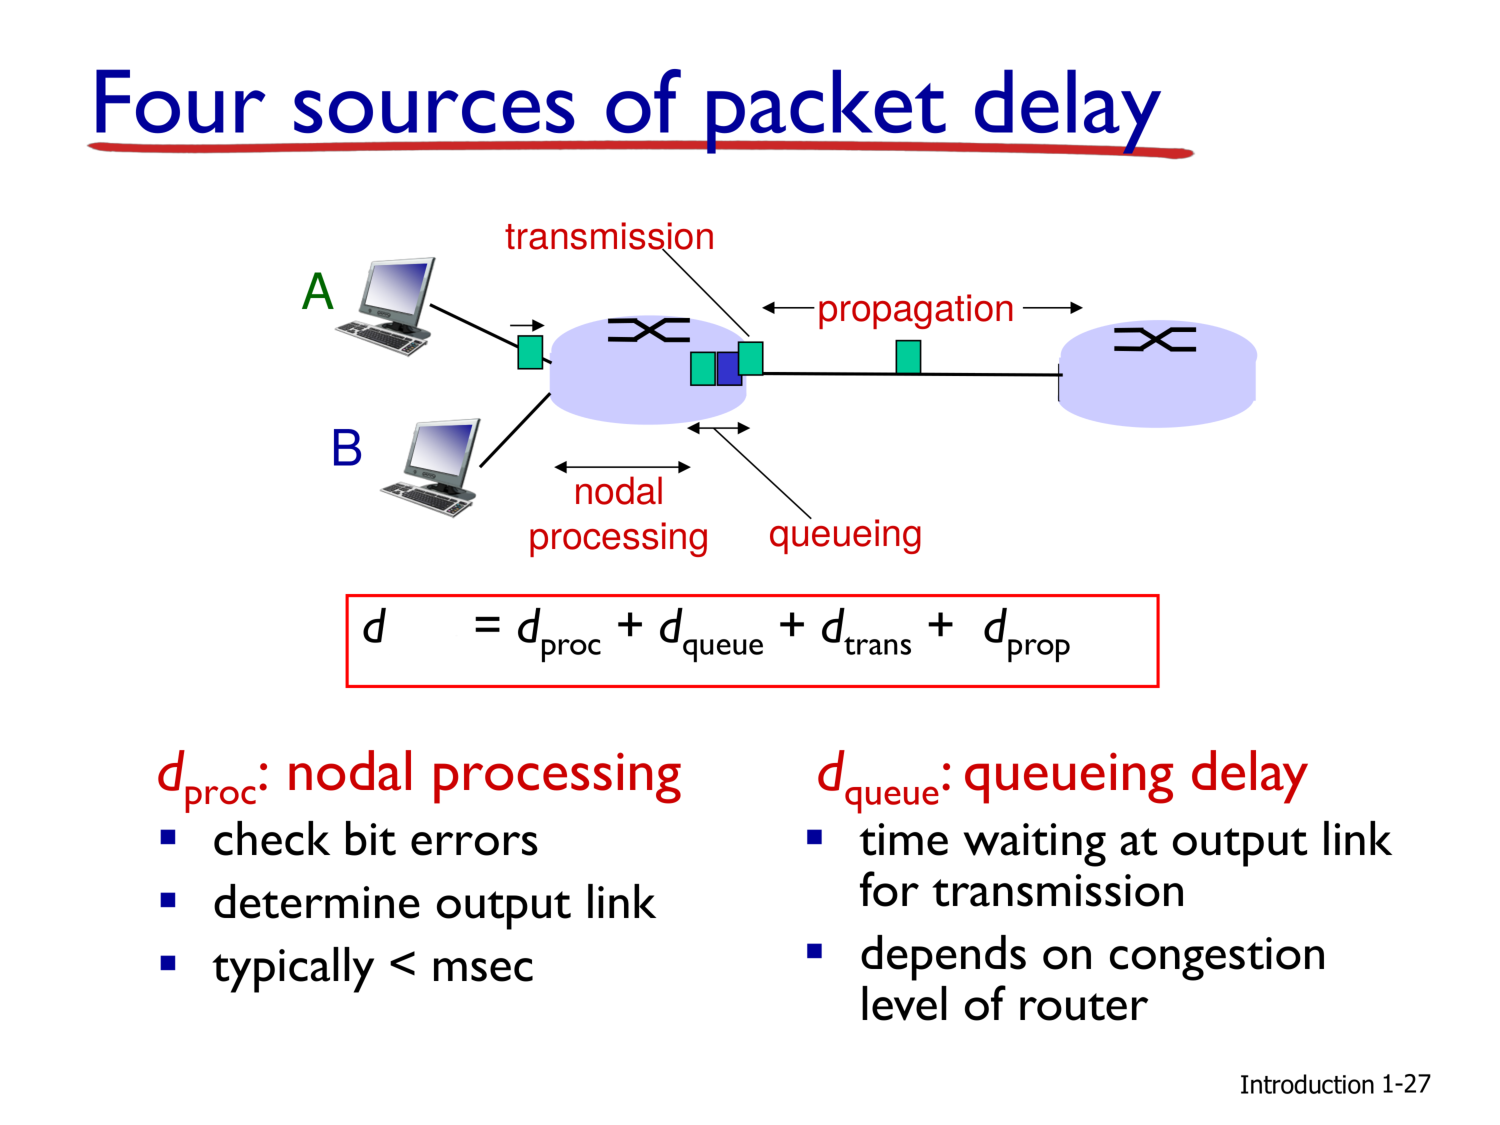
\includepdf[page=1]{slides2.pdf}
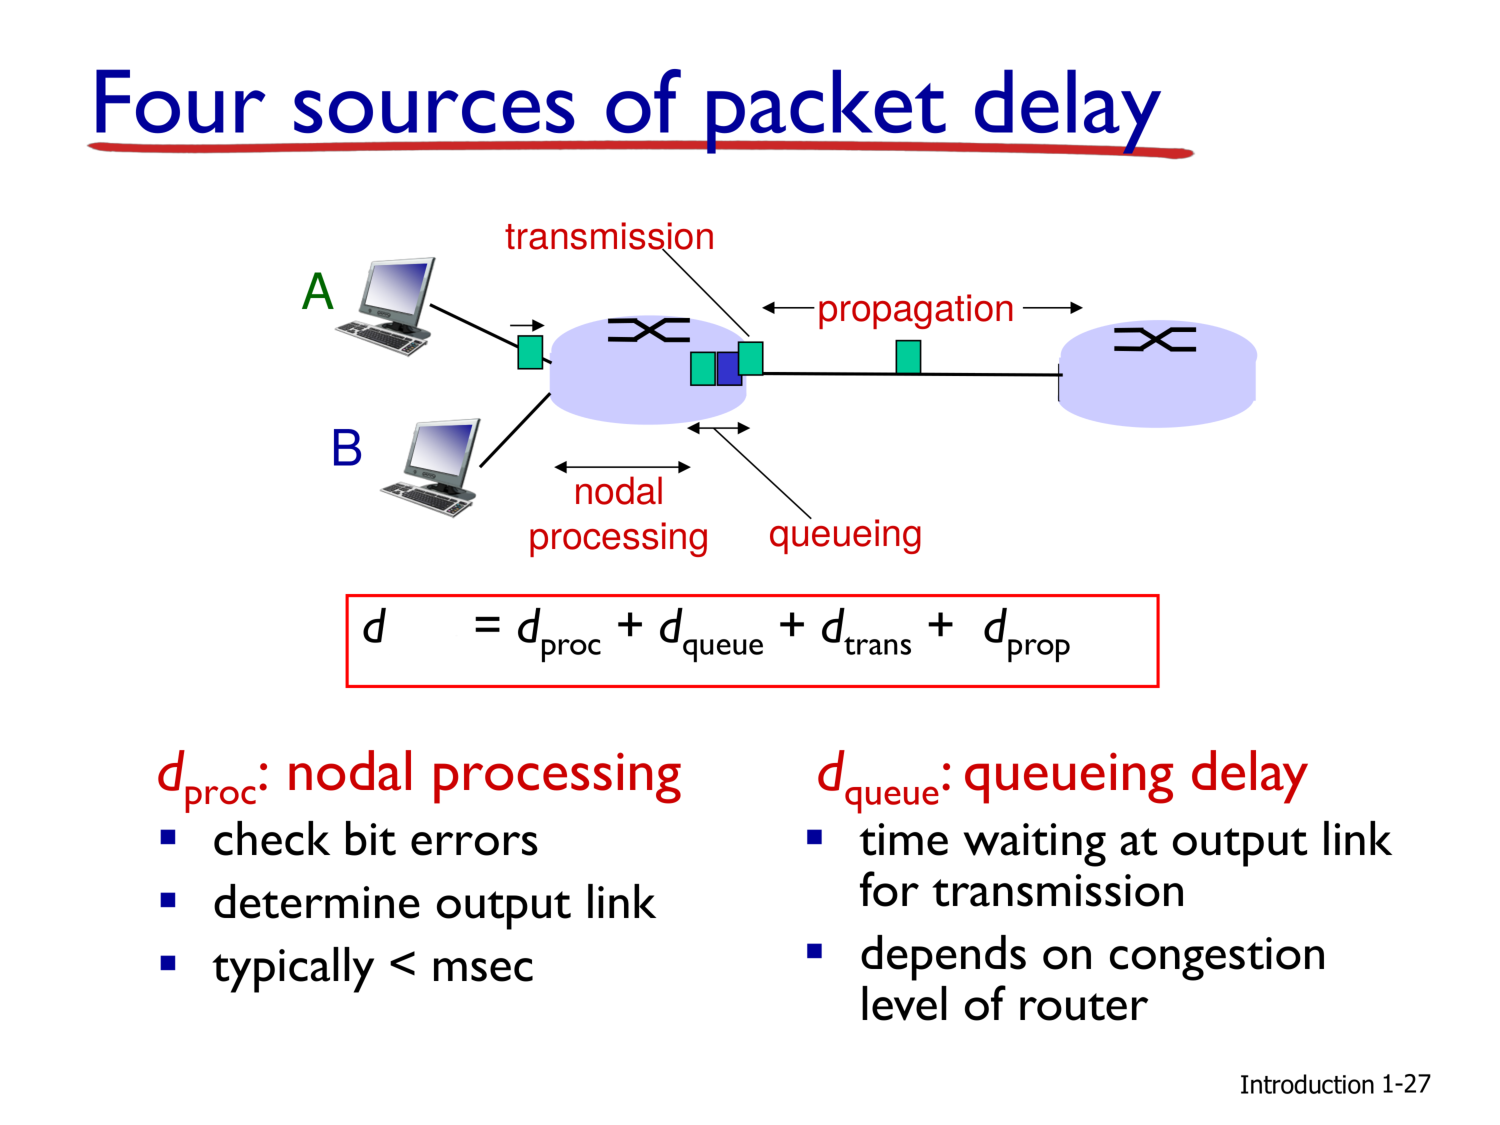
\includepdf[page=2]{slides2.pdf}
The processing delay is how much you get bogged down processing stuff. An example of this is looking shit up in the routing table. Really got devices use a TCAM to speed up this look up by expanding the prefix and store in in a CAM (content addressable memory). CAM works by letting you present content and use that too look up something else instead of requiring you to know the address of the thing you're looking for. This memory is super expensive so lots of the cost of a network box goes into getting more TCAM. You can overflow your TCAM if you have large prefixes.

Propogation delay is delay introduced by the physical distance you are covering. We want to assume that shit is moving at the speed of light (it most definitly is not, but we assume so).


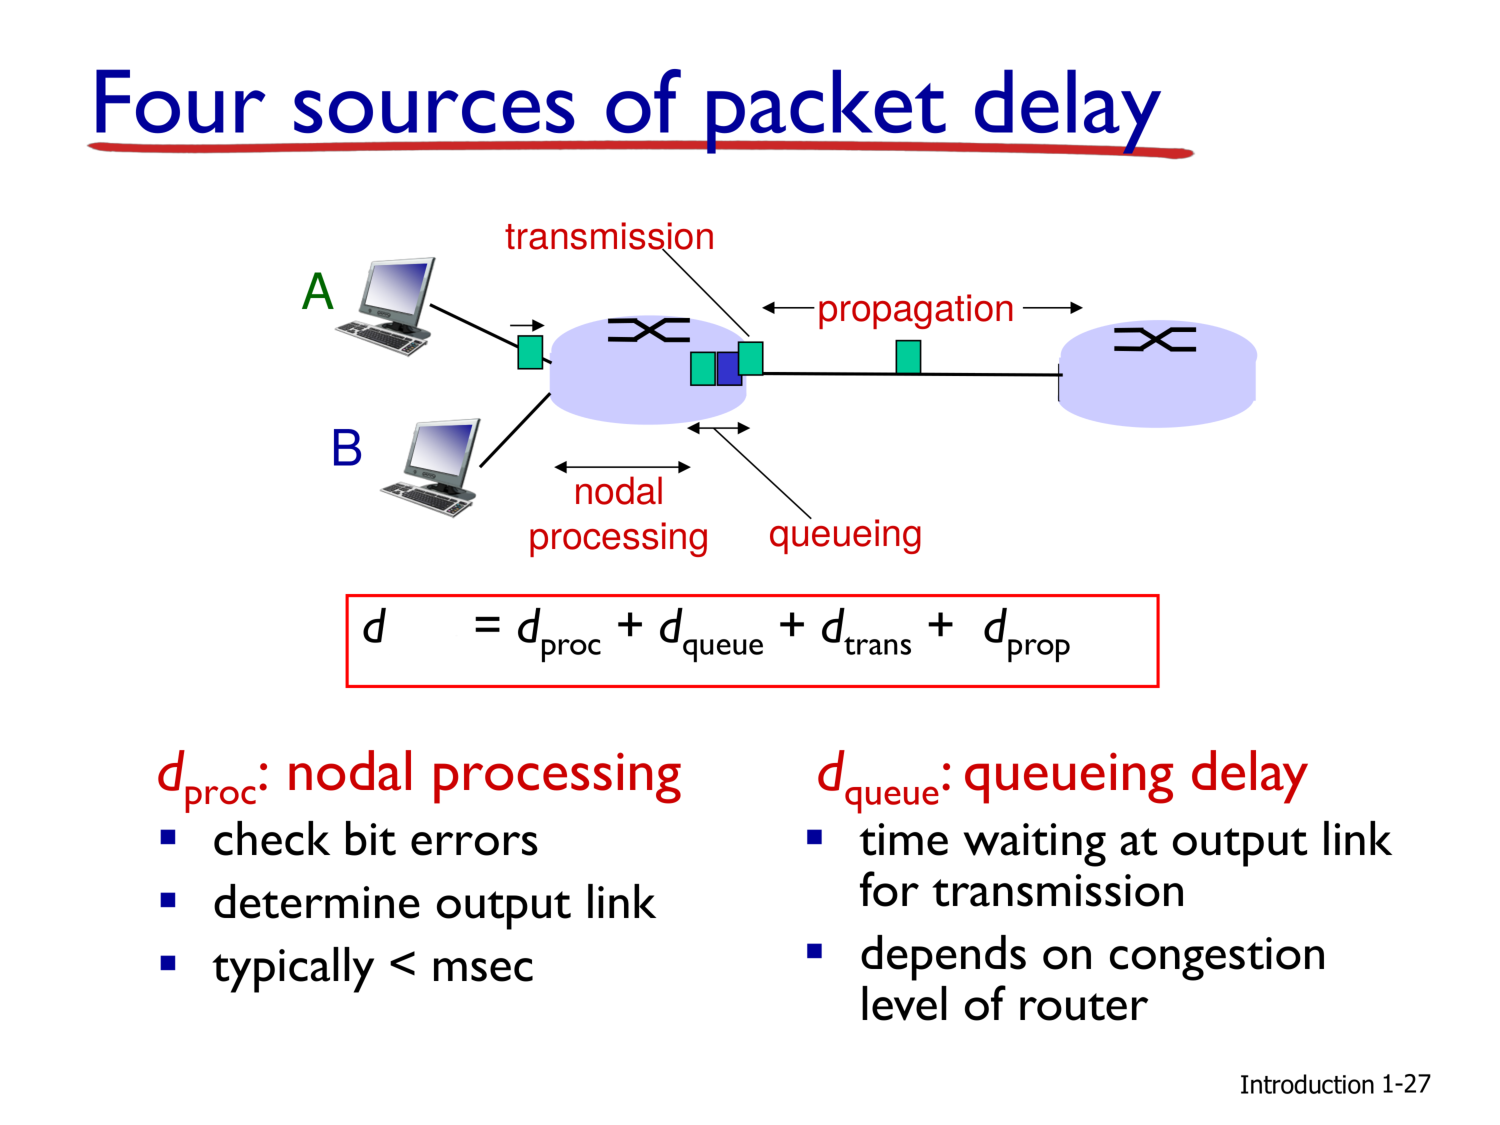
\includepdf[page=3]{slides2.pdf}
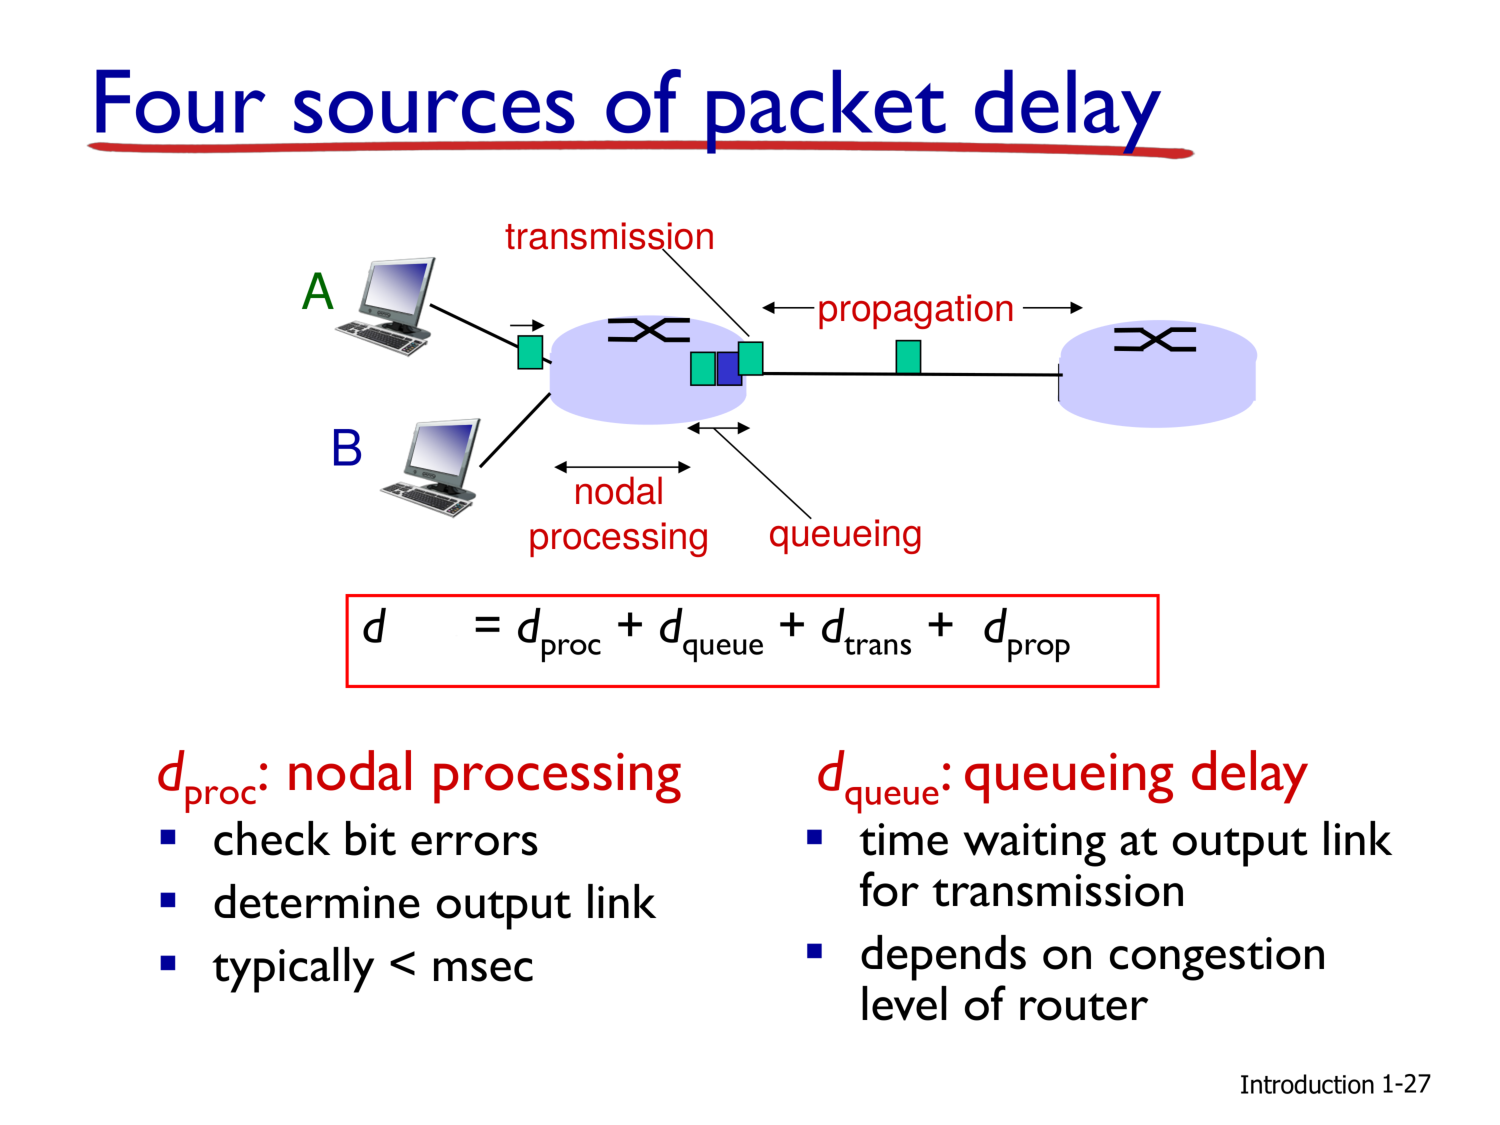
\includepdf[page=4]{slides2.pdf}
In this analogy we pretend that the processing delay is the toll booth and the speed of the car is the propogation delay. We want to know how long it takes all of the cars to reuinte at the toll booth. Basically the point of this is to show that the propagation delay is dominant.

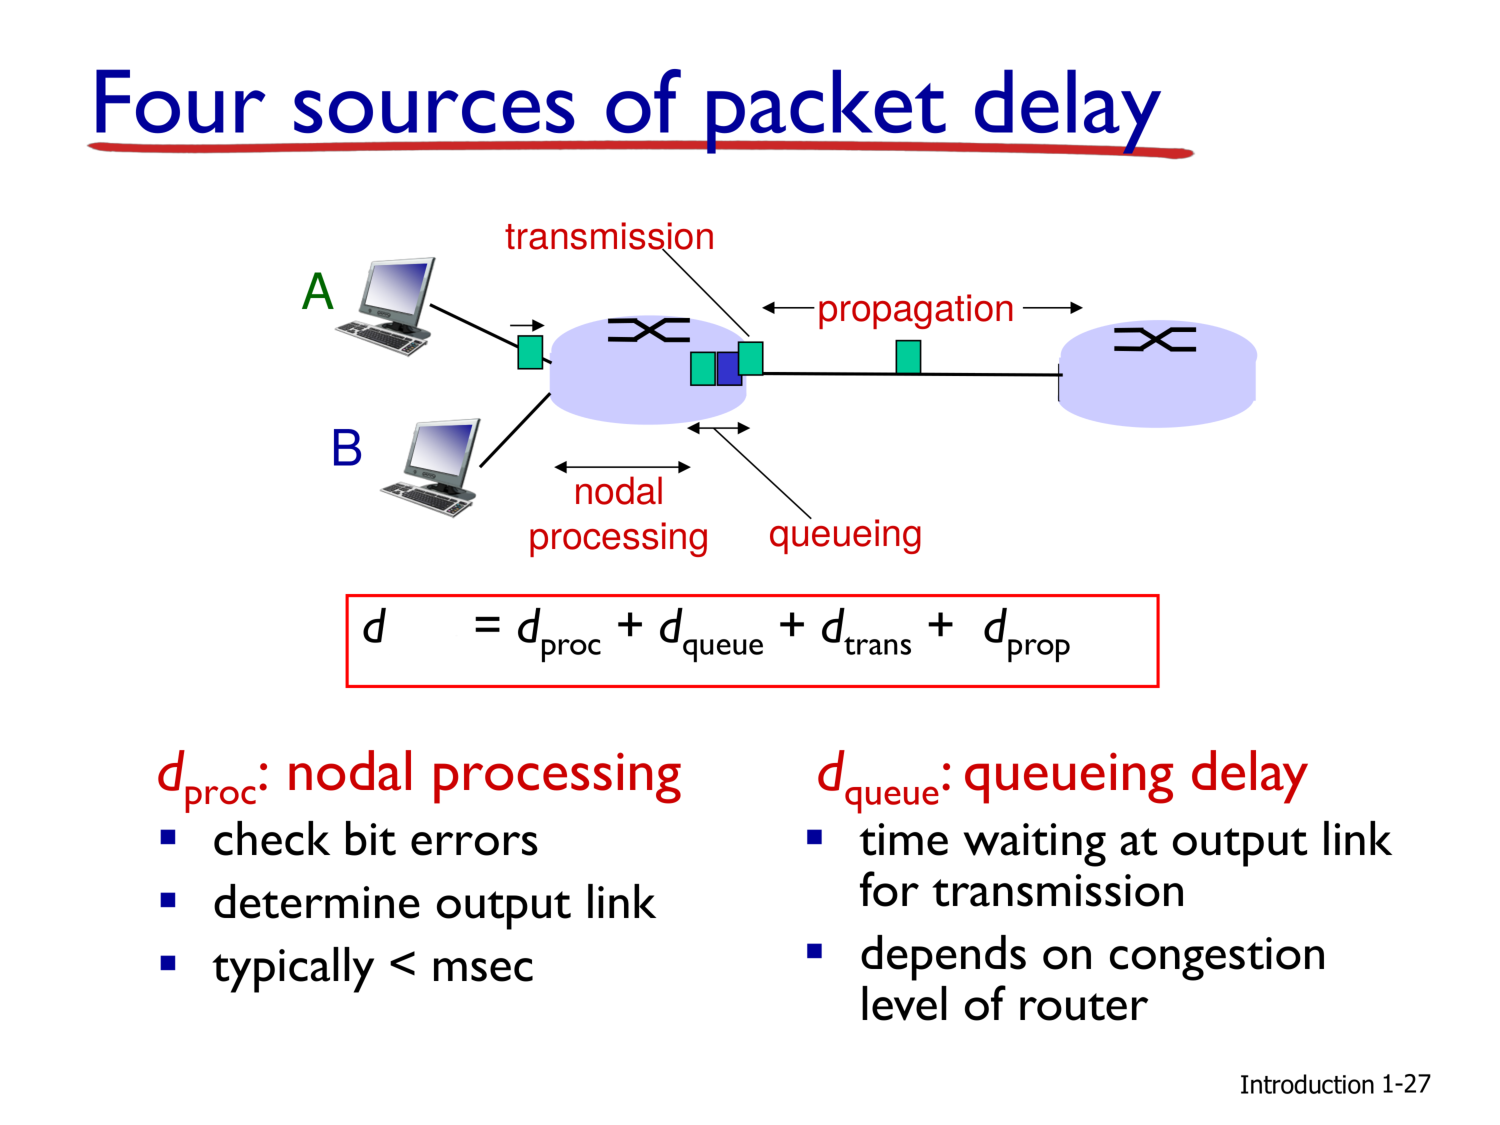
\includepdf[page=5]{slides2.pdf}
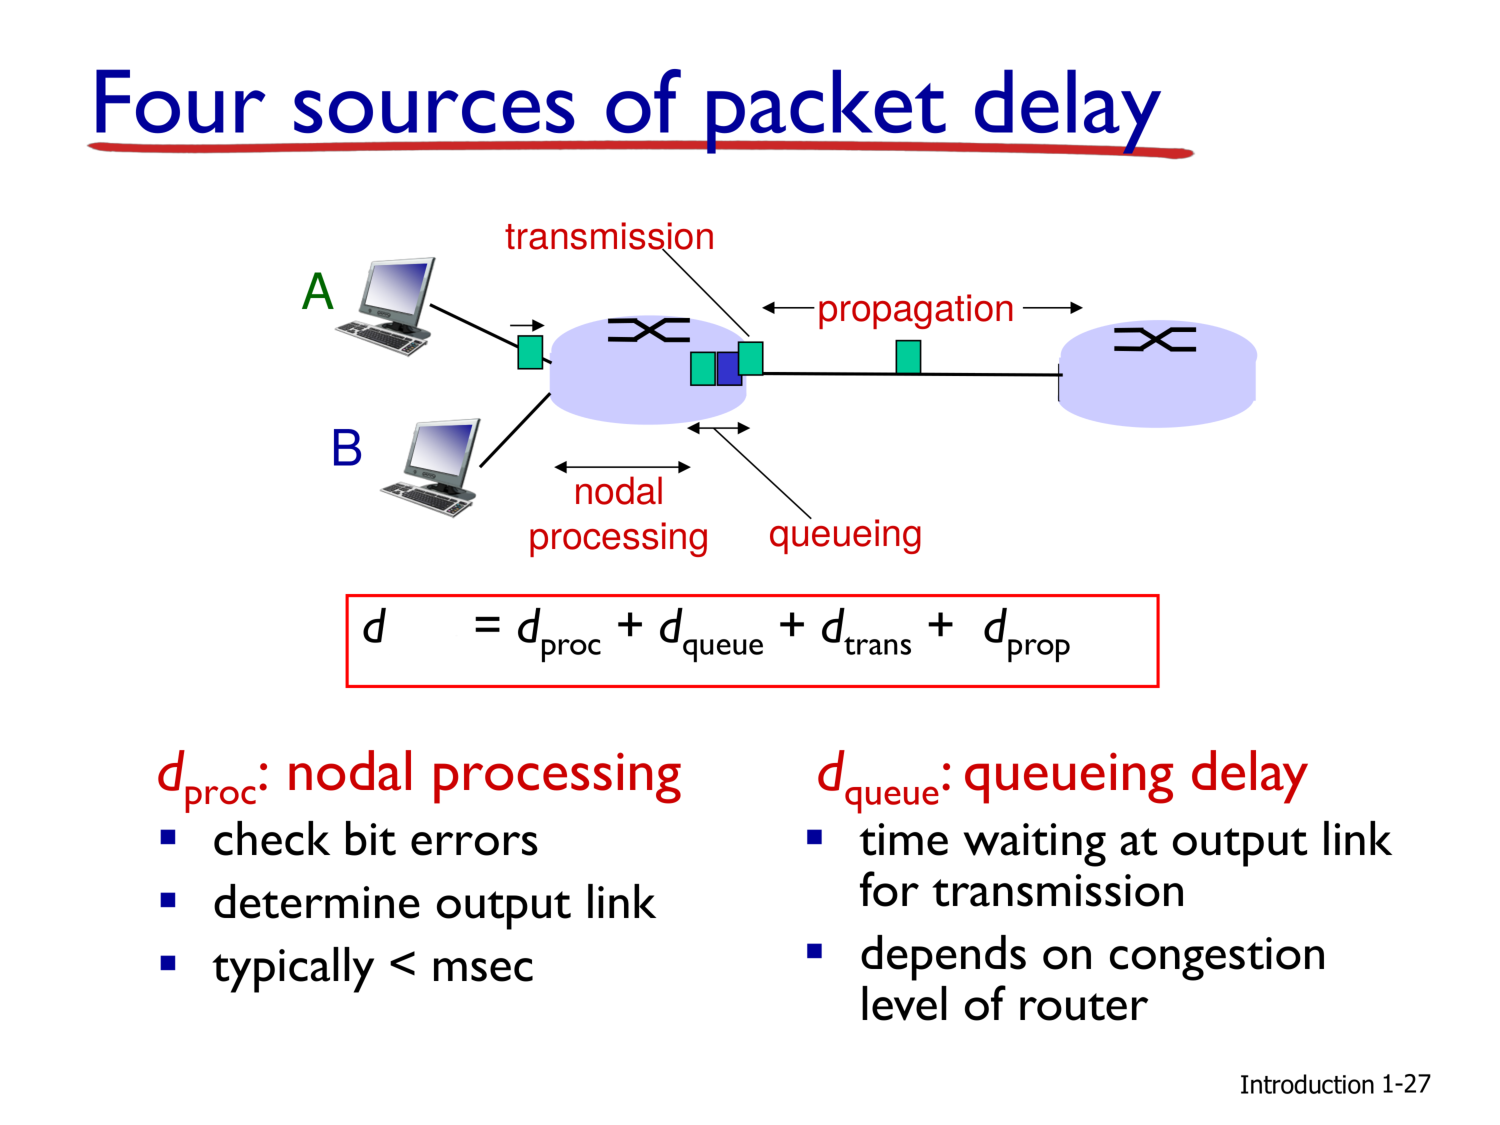
\includepdf[page=6]{slides2.pdf}
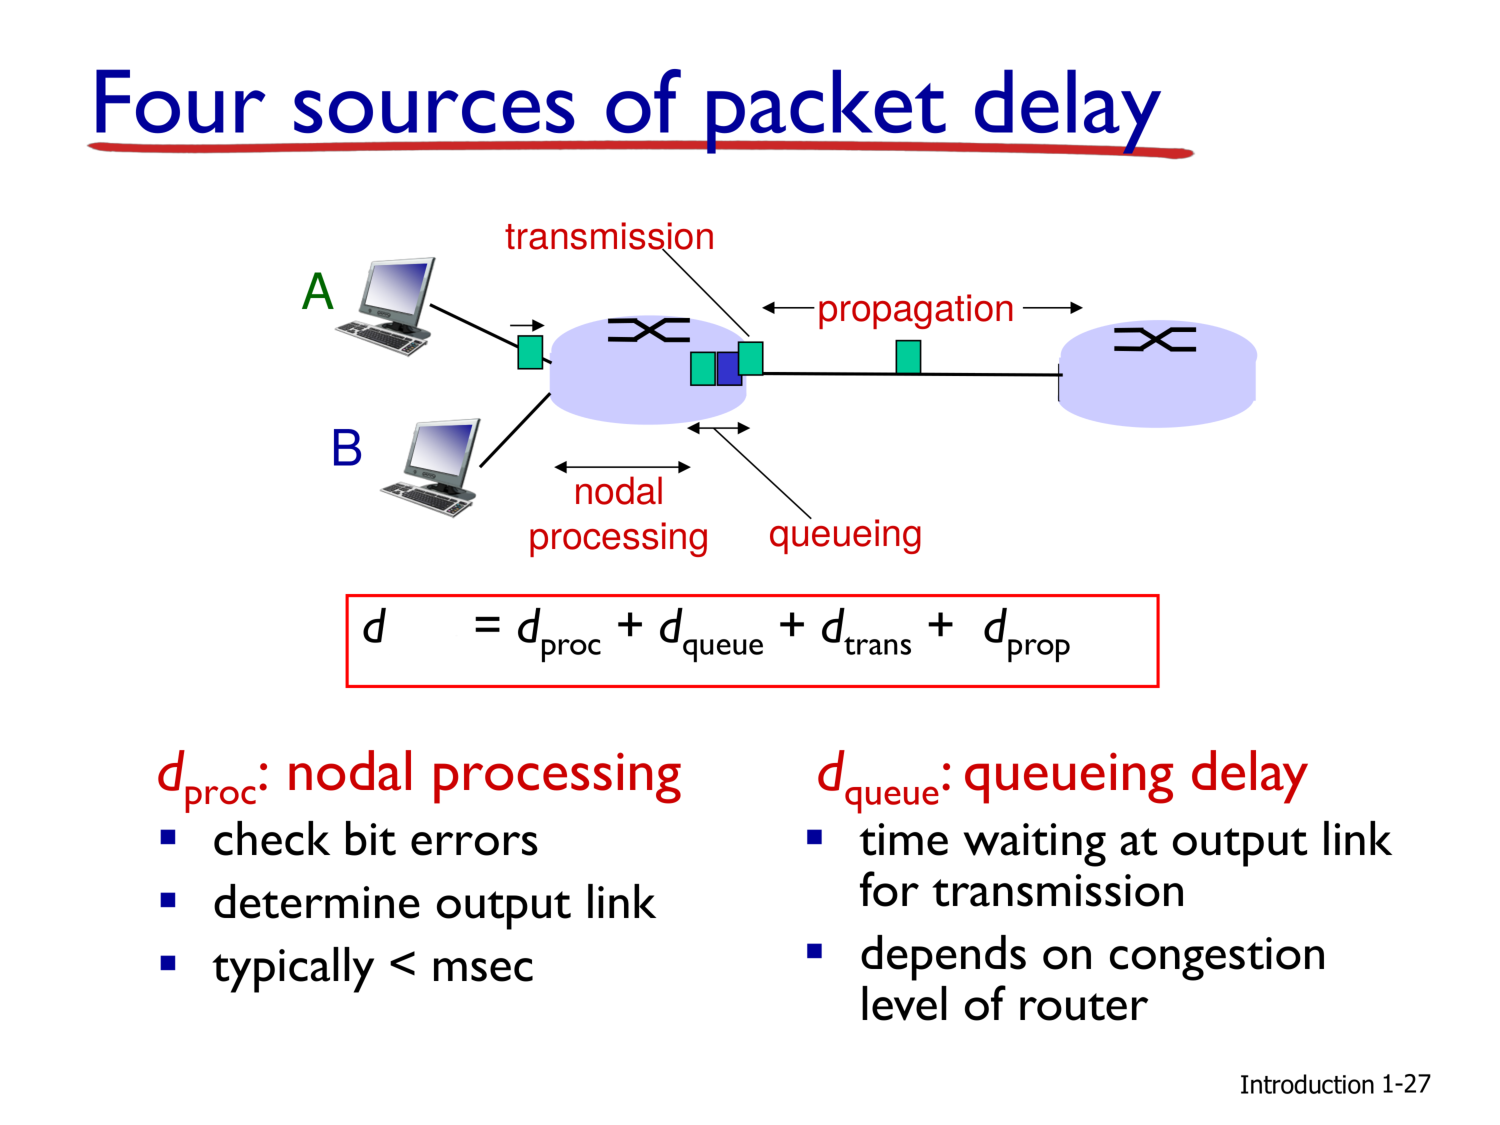
\includepdf[page=7]{slides2.pdf}
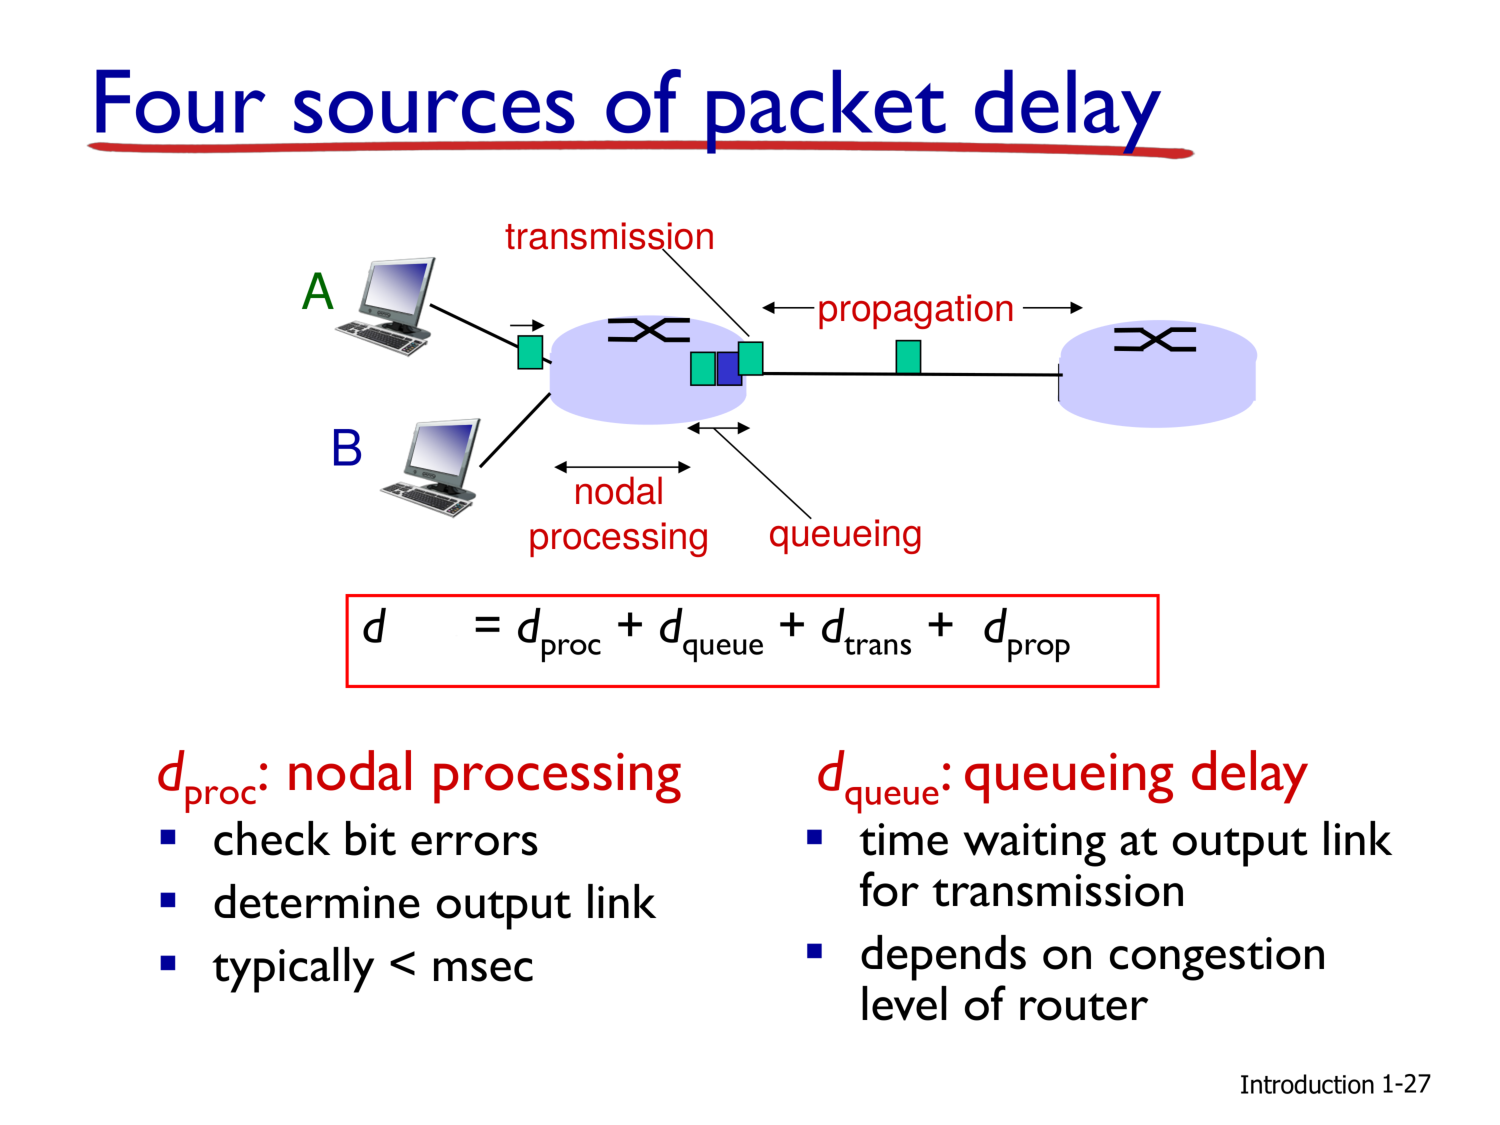
\includepdf[page=8]{slides2.pdf}
Packets that arrive to a full queue are dropped (although you can define any strategy for this). 
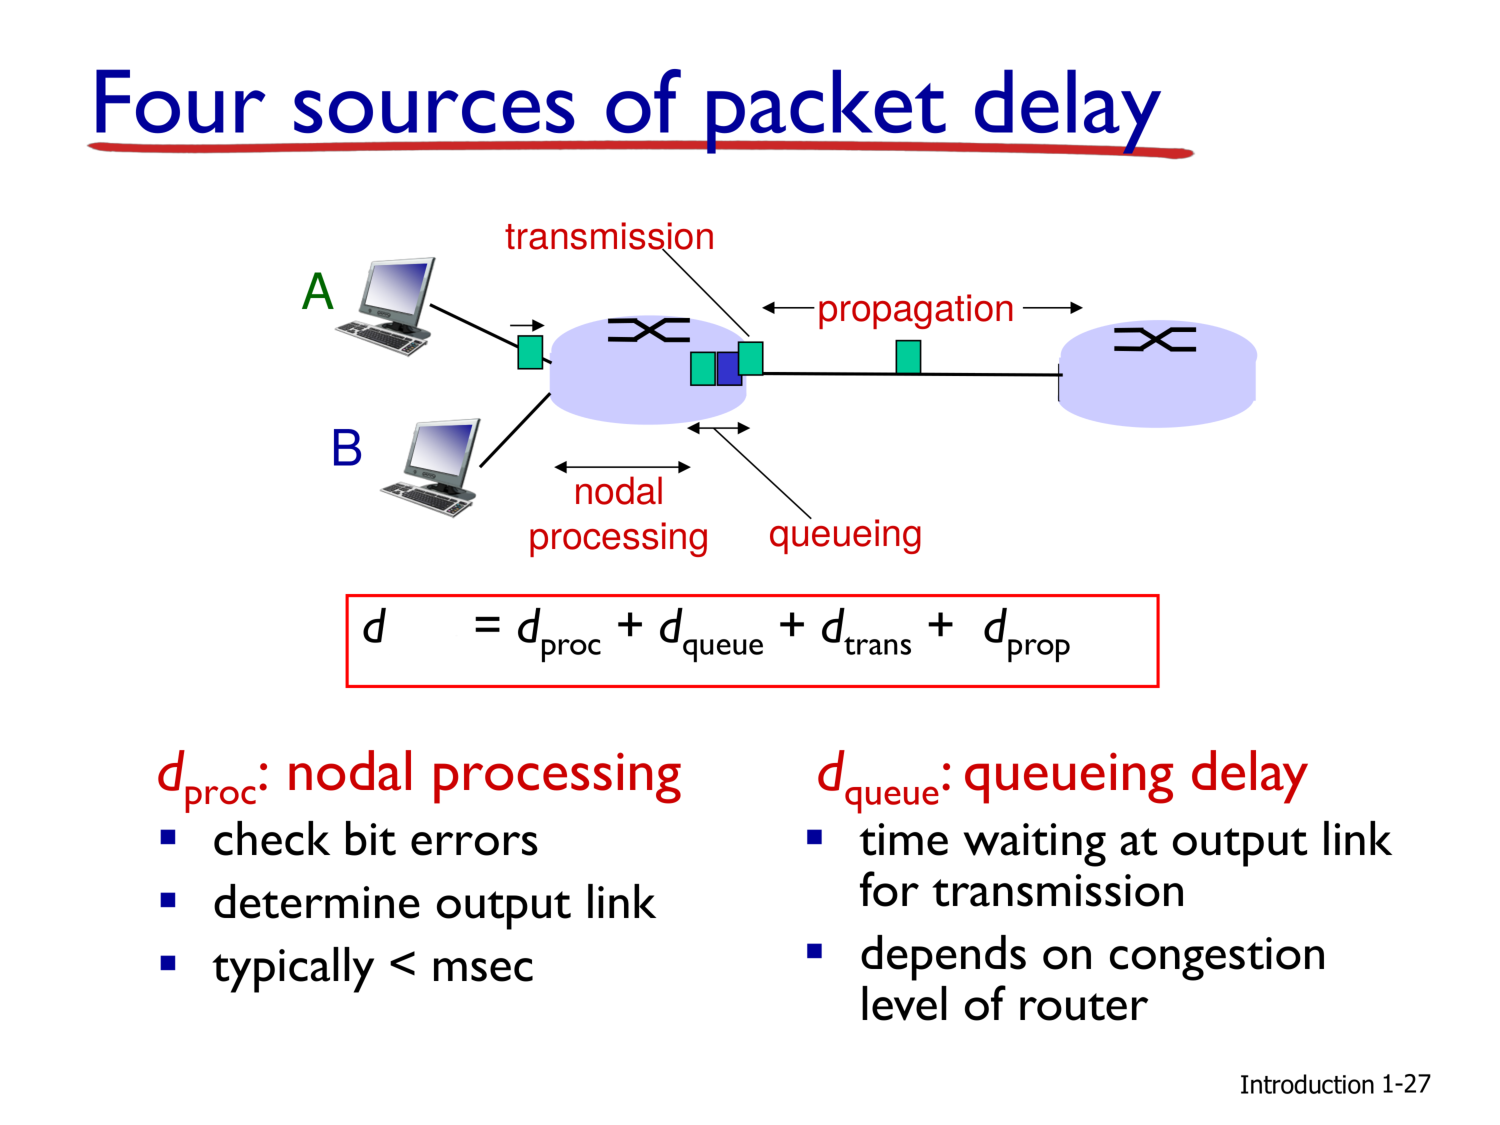
\includepdf[page=9]{slides2.pdf}
Throughput is the number of bits per unit of time. 

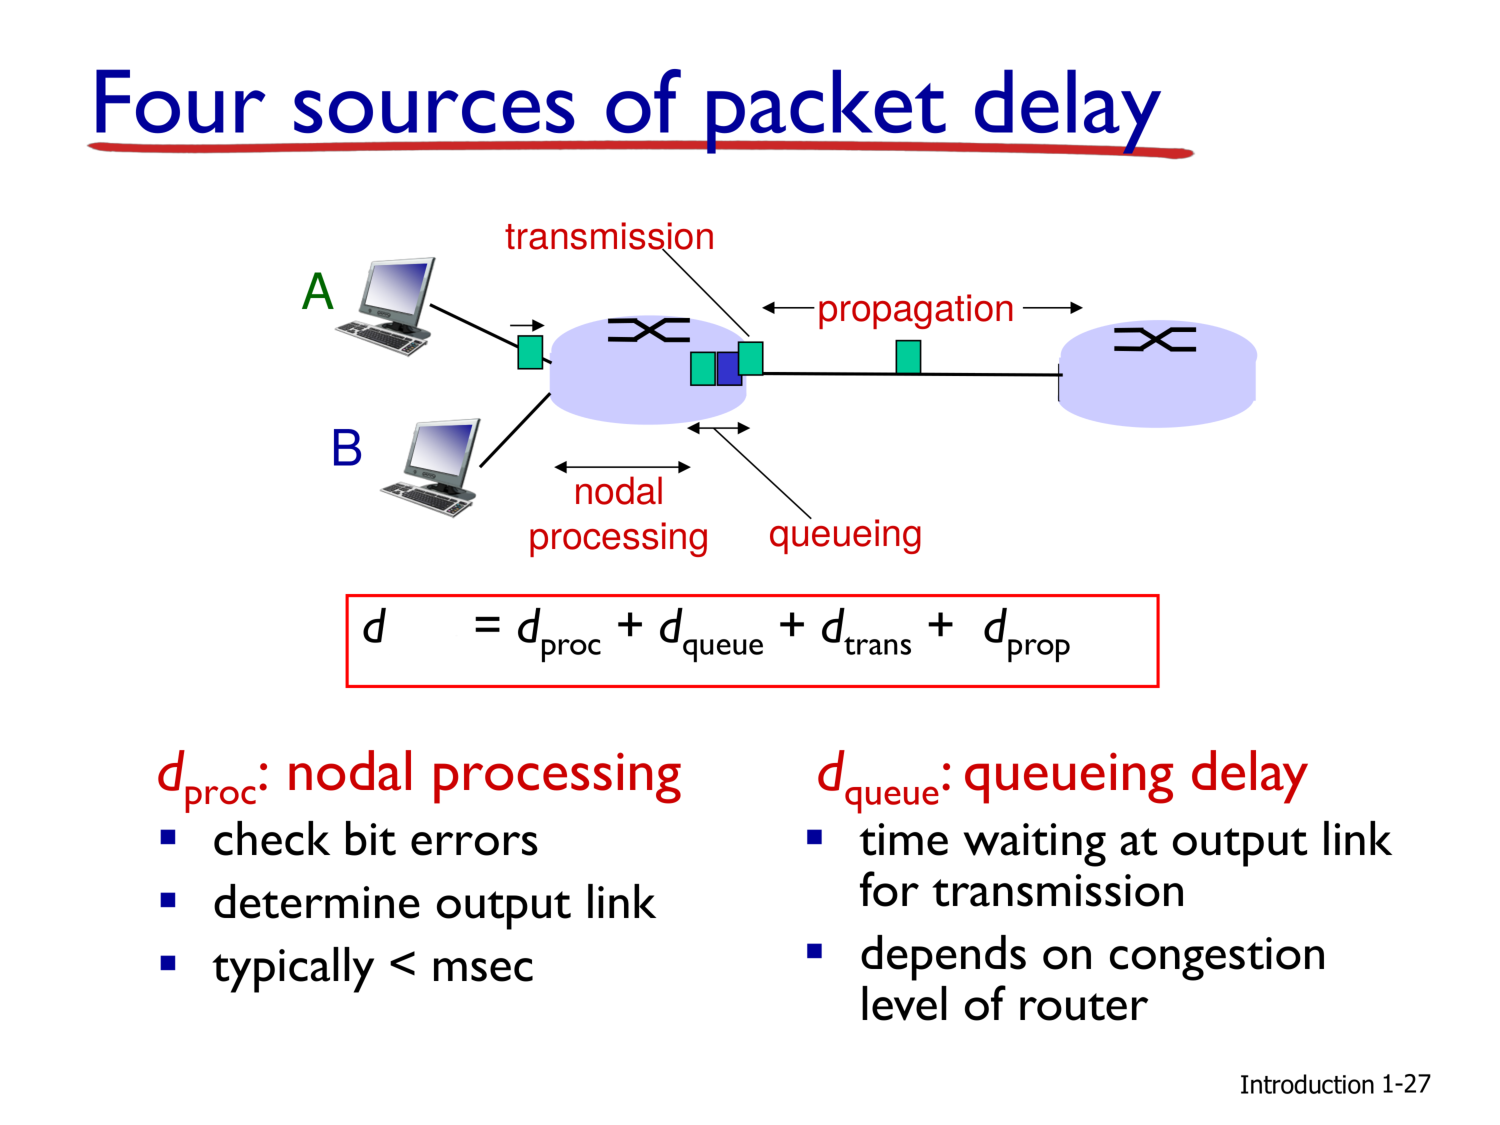
\includepdf[page=10]{slides2.pdf}
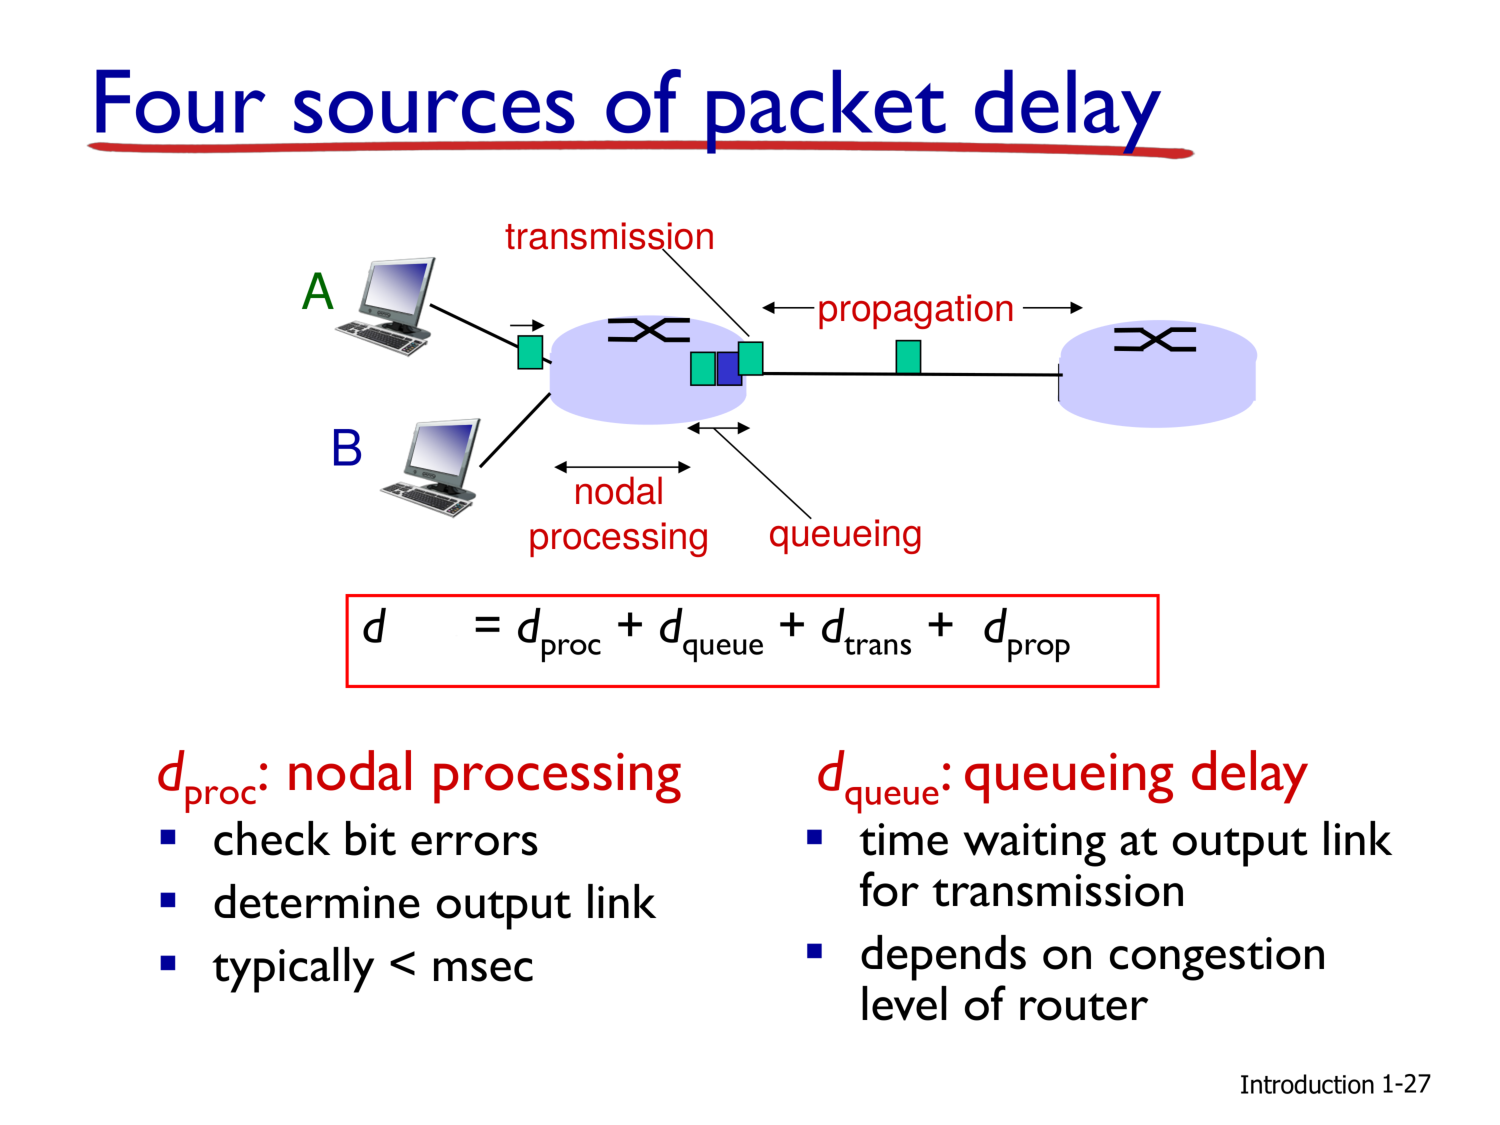
\includepdf[page=11]{slides2.pdf}


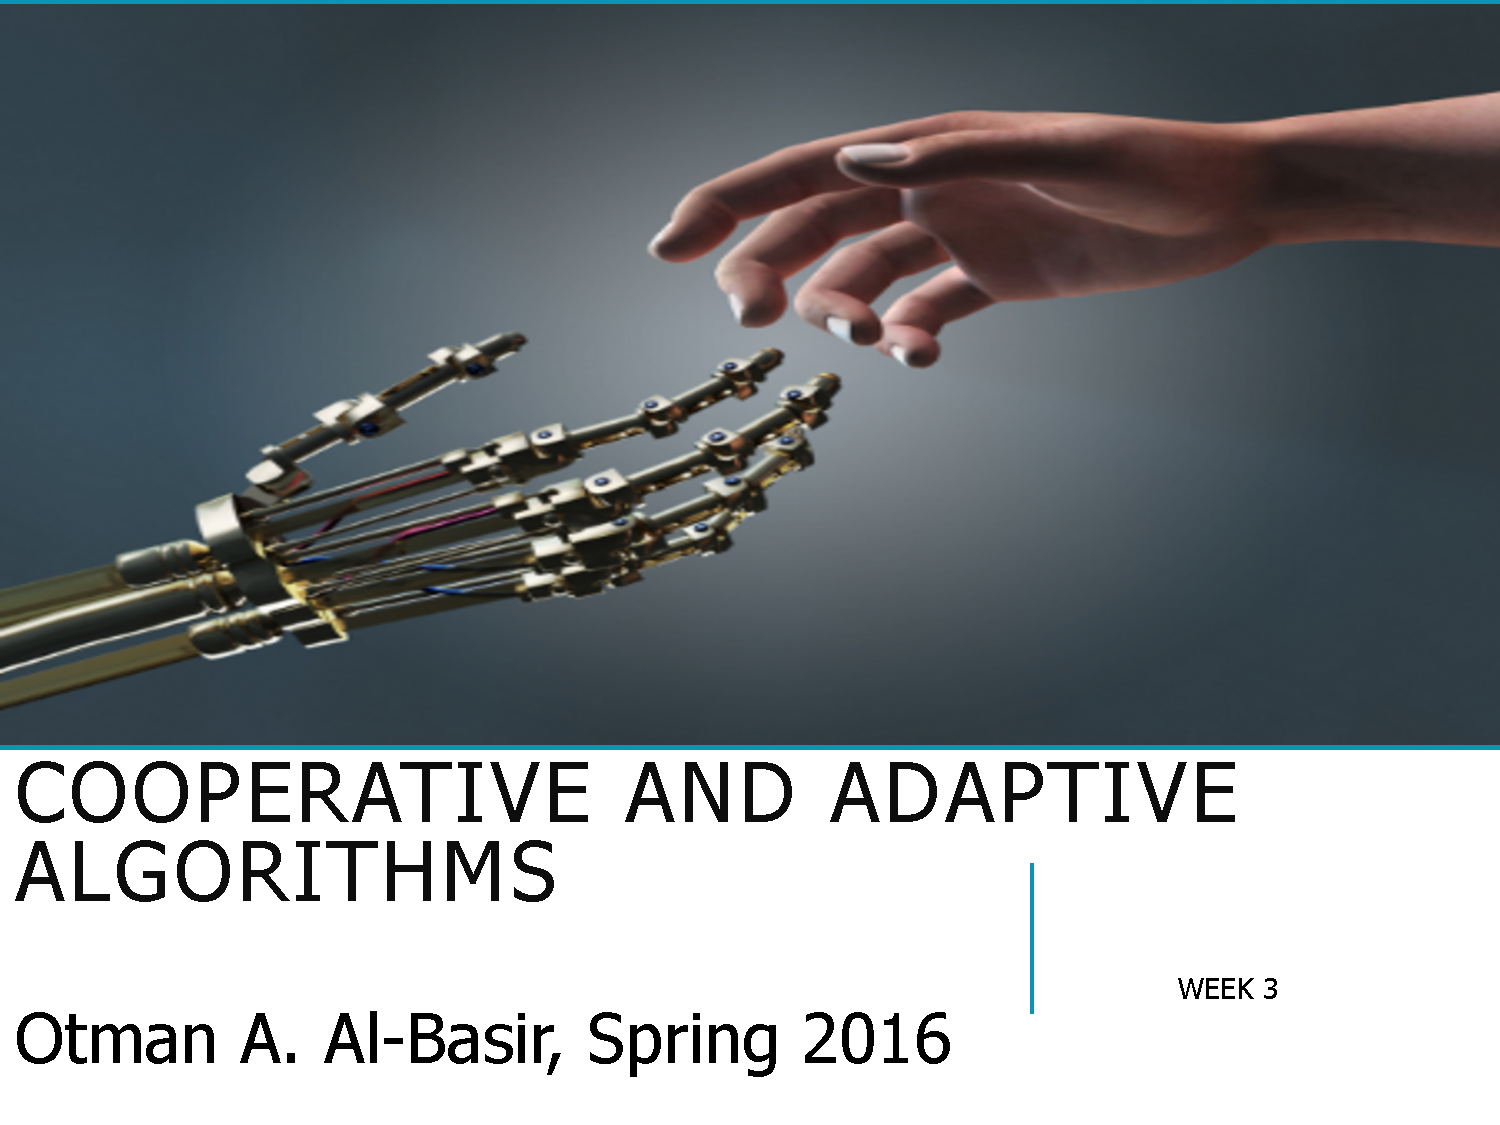
\includepdf[page=37]{slides.pdf}
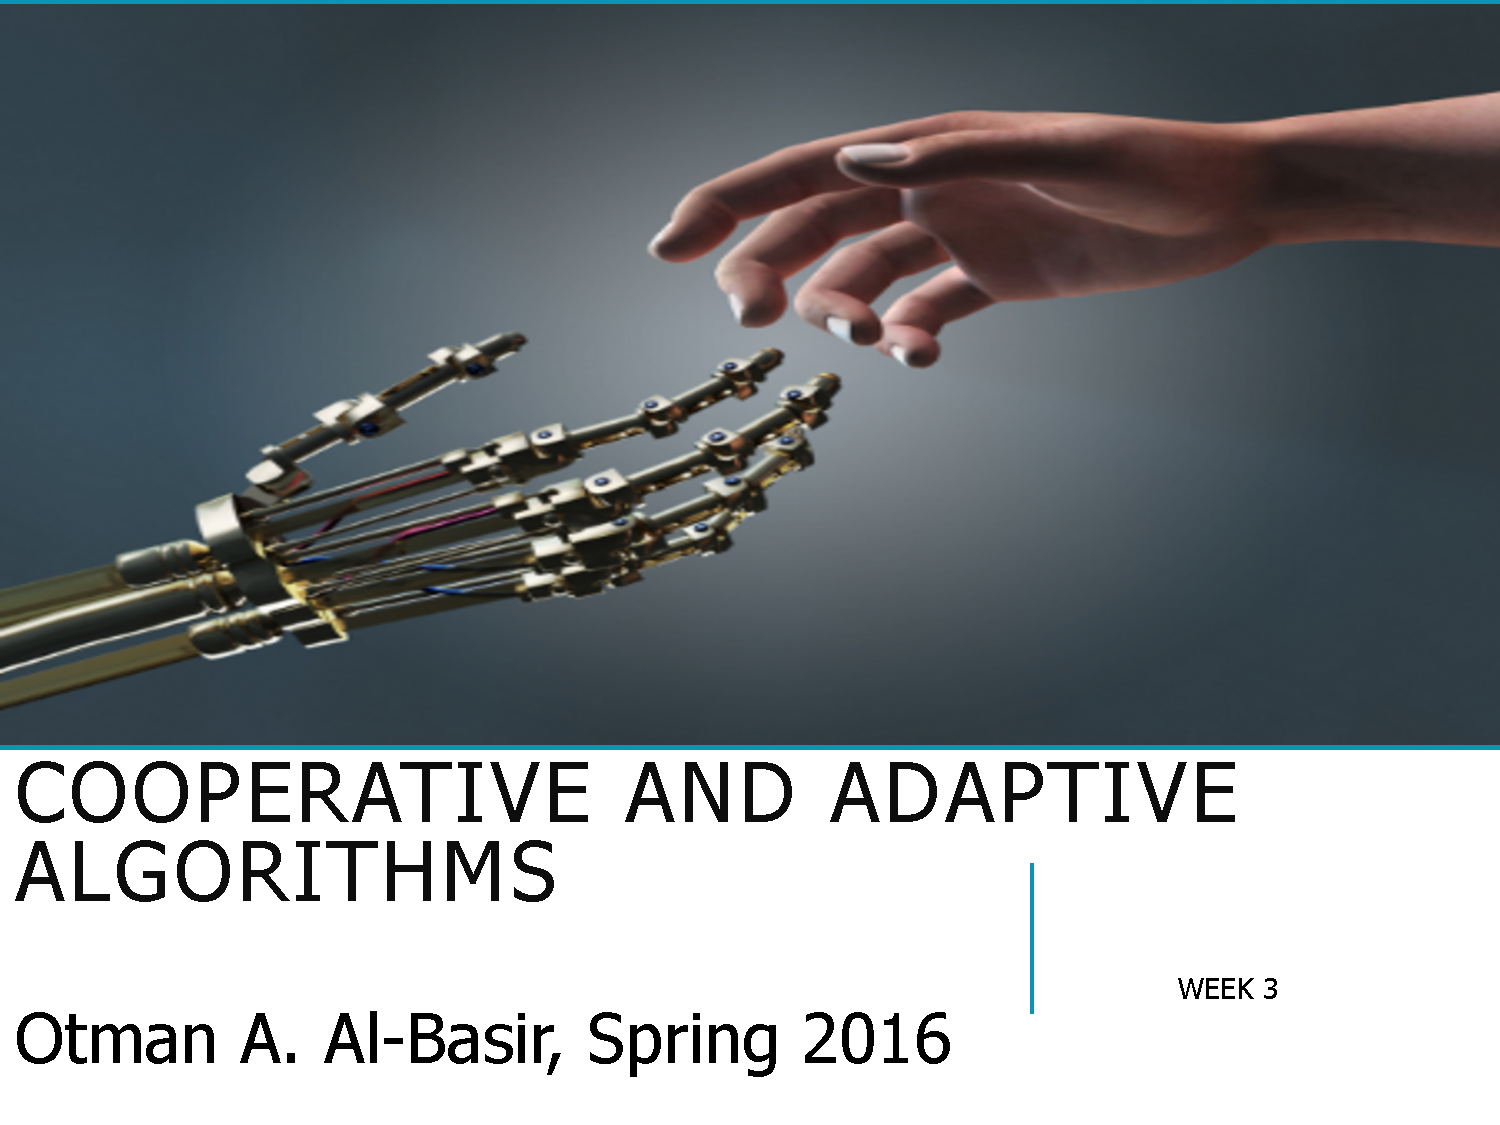
\includepdf[page=38]{slides.pdf}
We can make the utilization values very high by having the sender send indiscriminatly and only acknowledge one at a time. This will have super low throughput though.

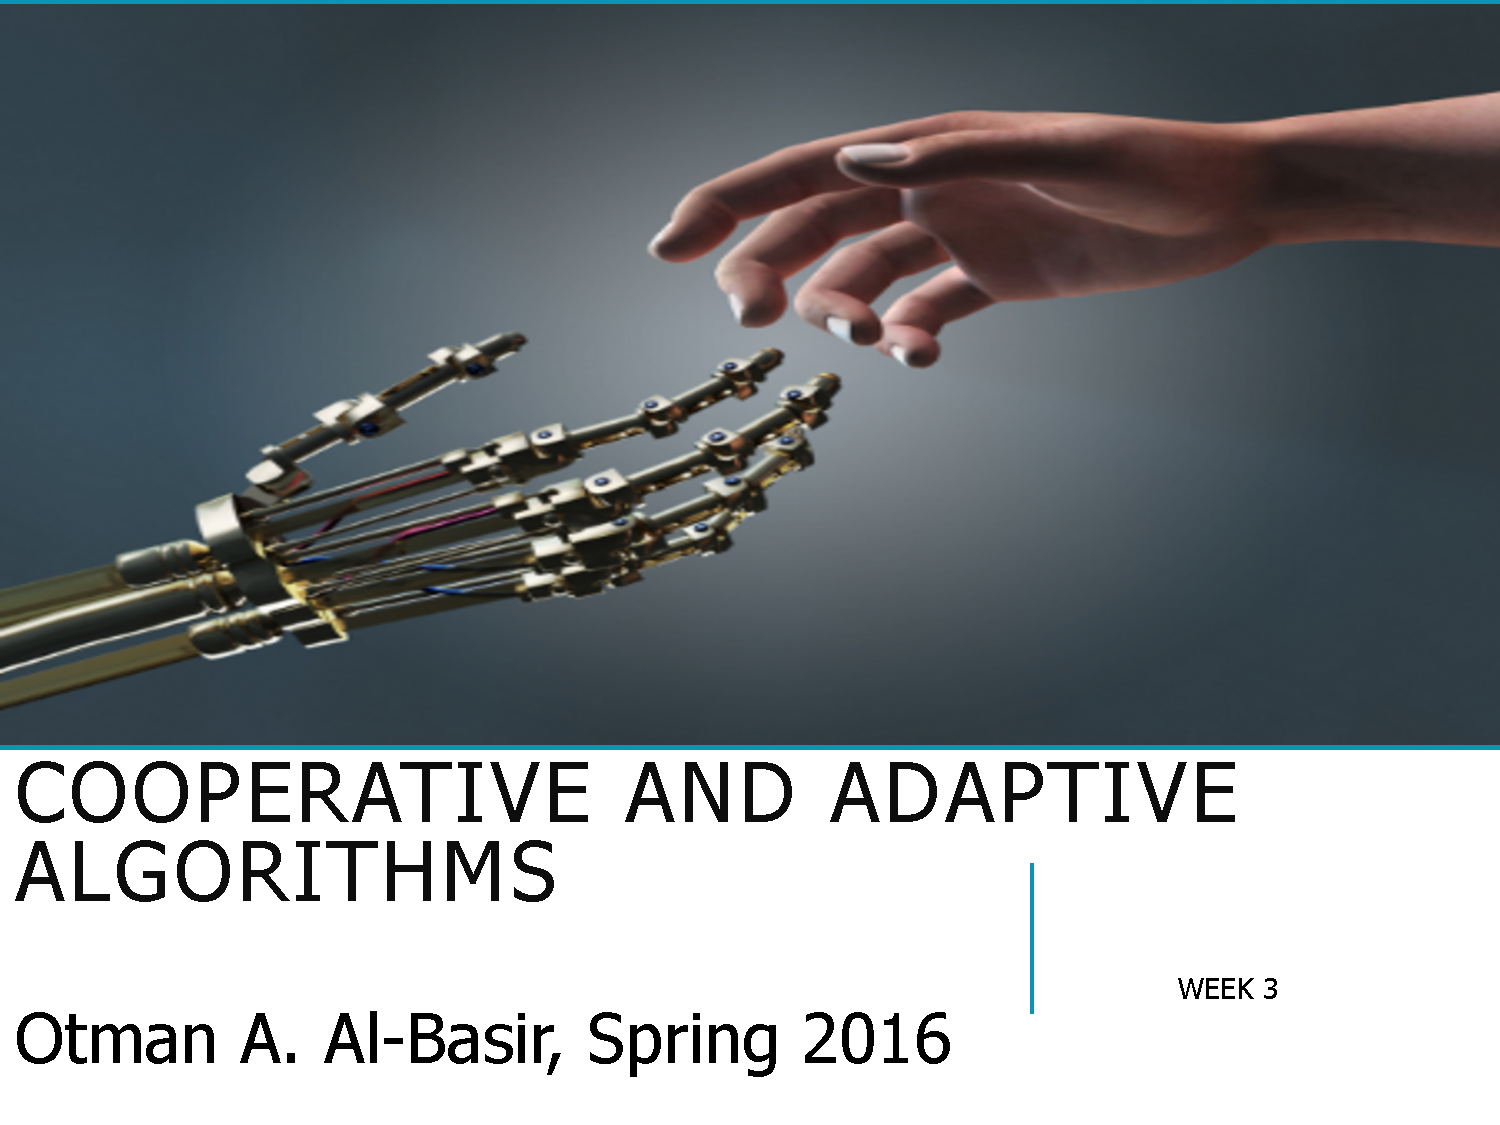
\includepdf[page=39]{slides.pdf}
Pipelining allows multiple packets being handled at the same time. So we have a sending window and receiving window that limit how many packets can be on the system at once. We then have to have a new sequence number for each packet (previously we had used only one bit).

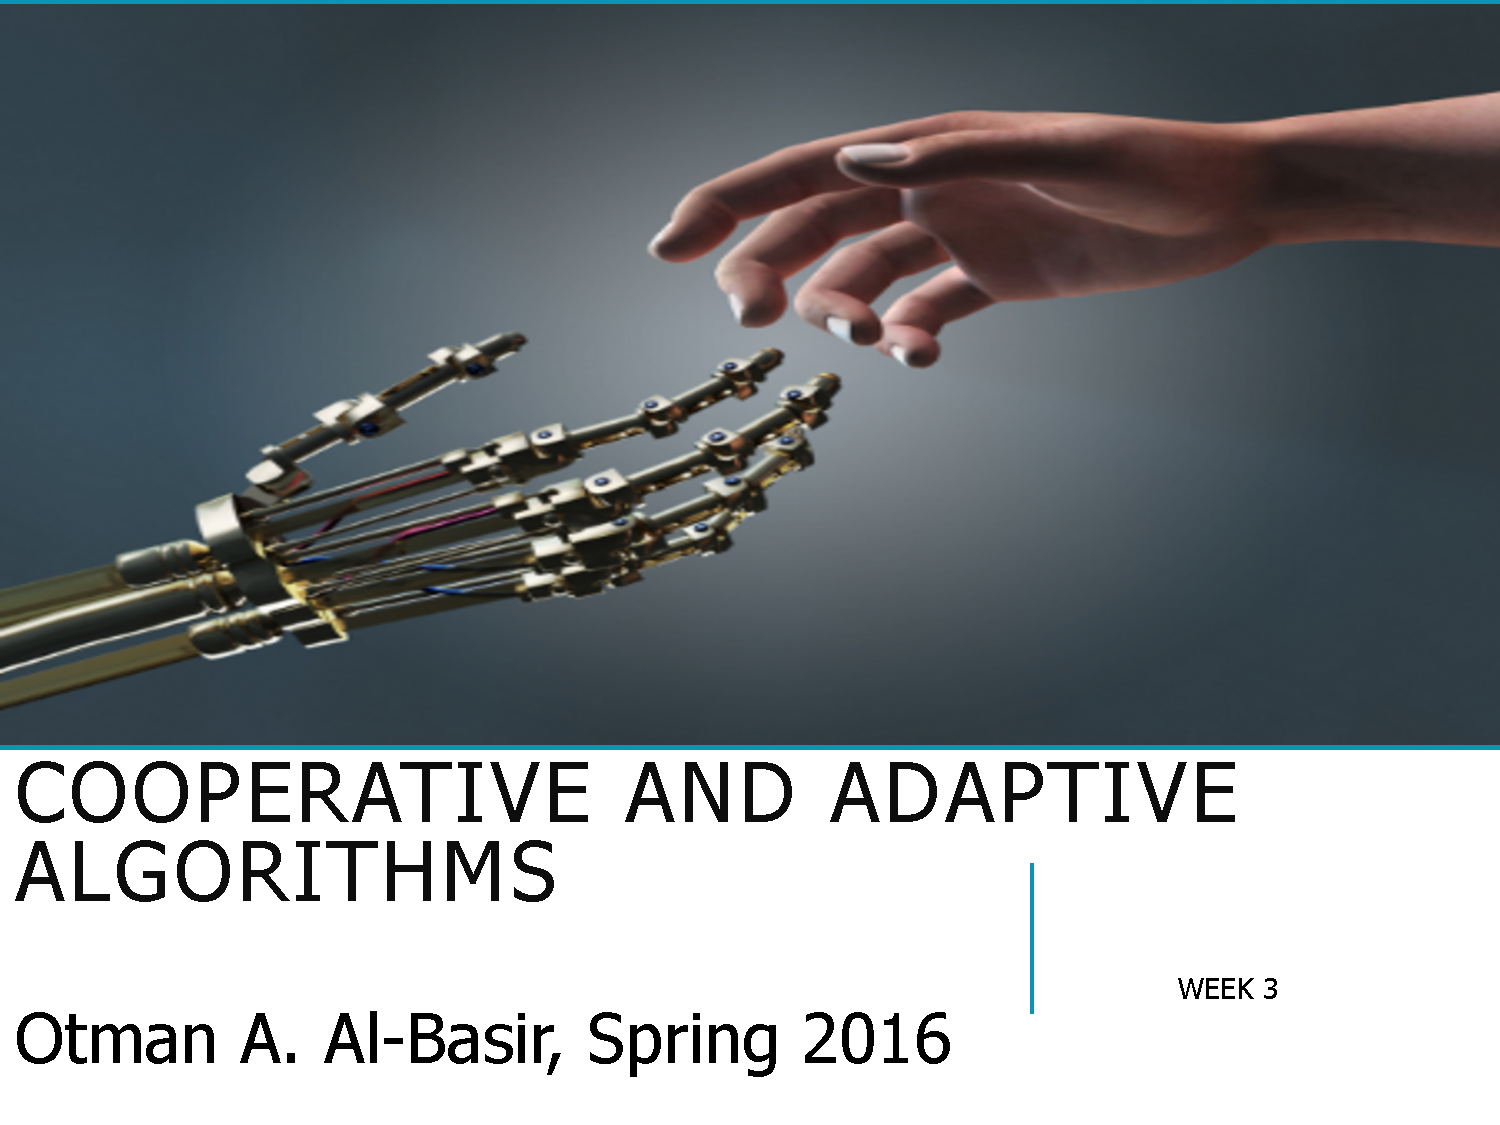
\includepdf[page=40]{slides.pdf}
The sender blindly sends three packets and waits. 

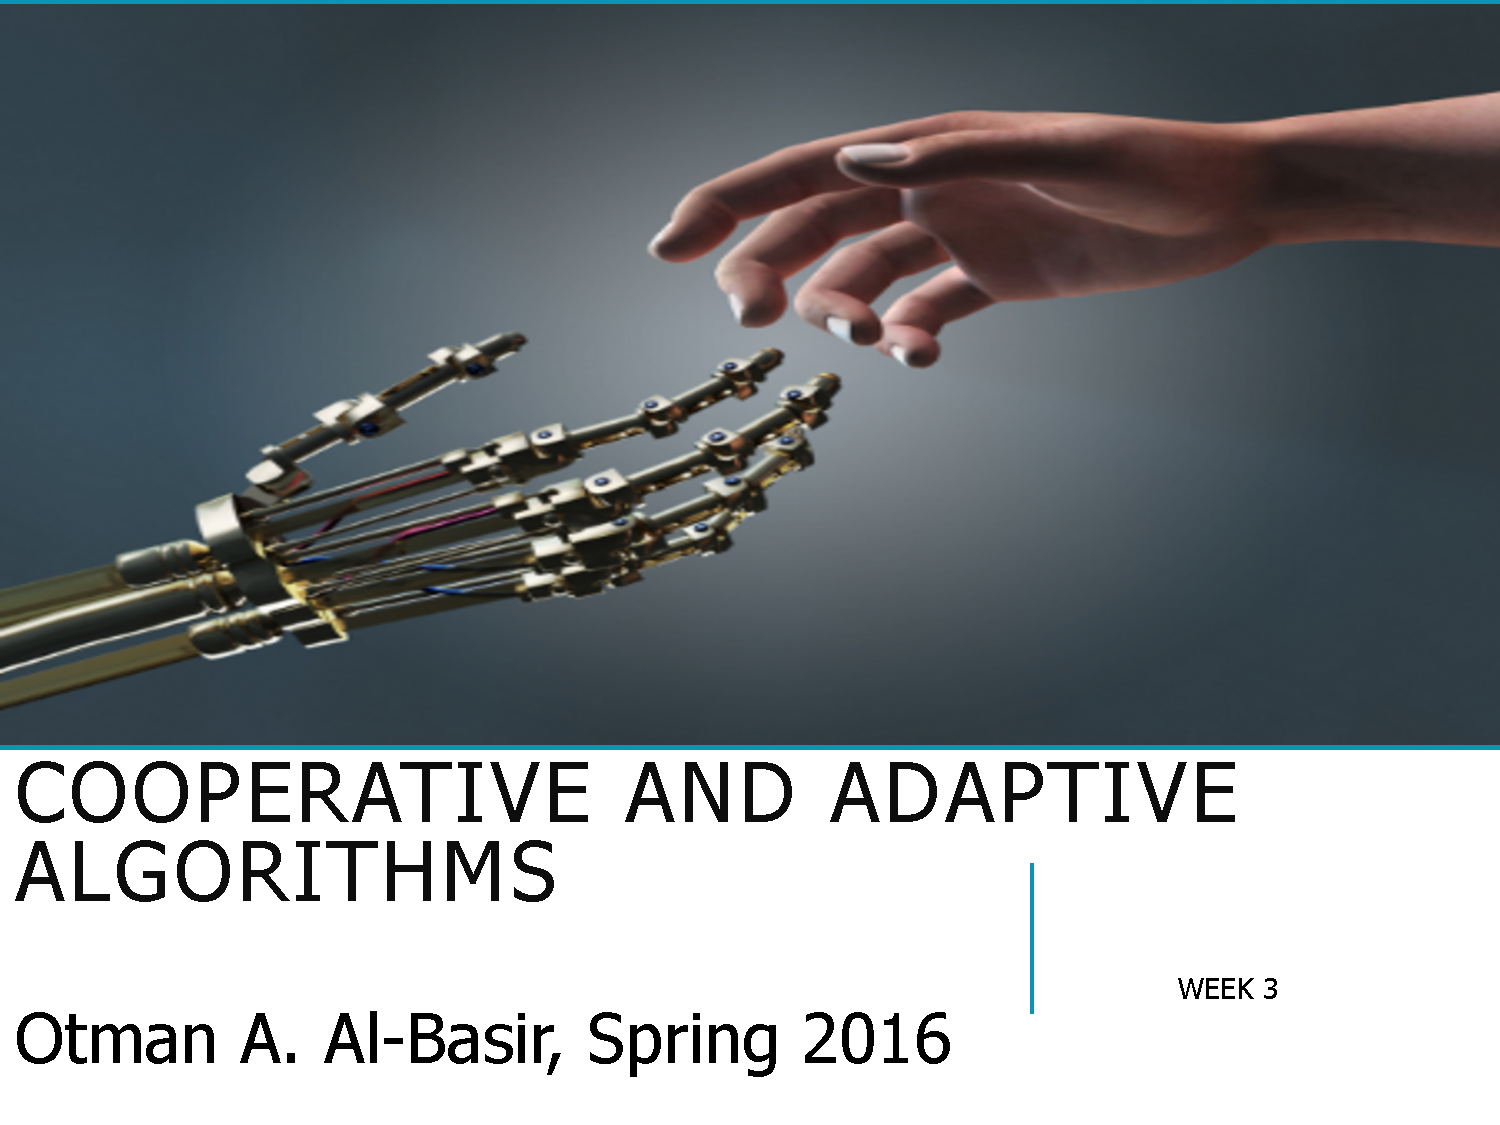
\includepdf[page=41]{slides.pdf}
The receiver sends a cumulative acknowledge, so only one ACK per N packets (waits until it has received all of them). So if it received 1, 2, and 4 it will only ACK 2 because there is a gap. We only have a timer for the oldest unacked packet.

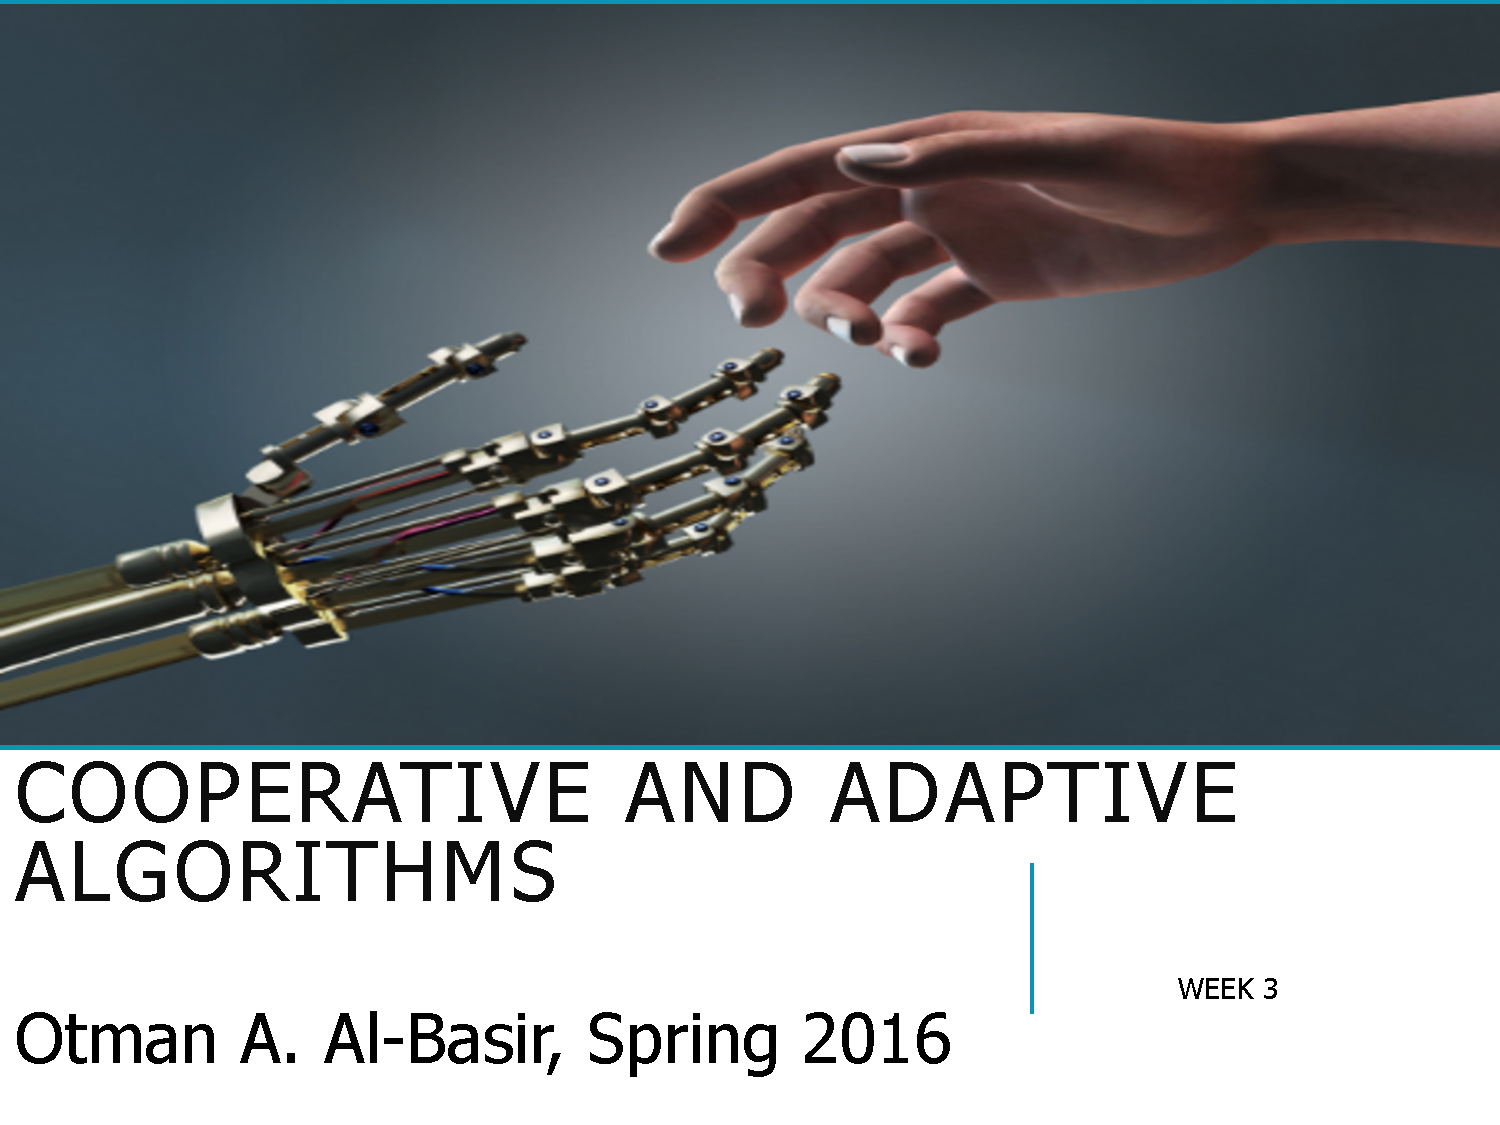
\includepdf[page=42]{slides.pdf}
There are two pointers, one at the oldest unacked packet and one at the next packet to be sent. This slide shows a set of sequence numbers. If you send to a node currently blocked on waiting for an ACK then it just returns an error because it cannot buffer any more.

In the sample code you have there is a reasonably high probability to "do evil" (drop packets).

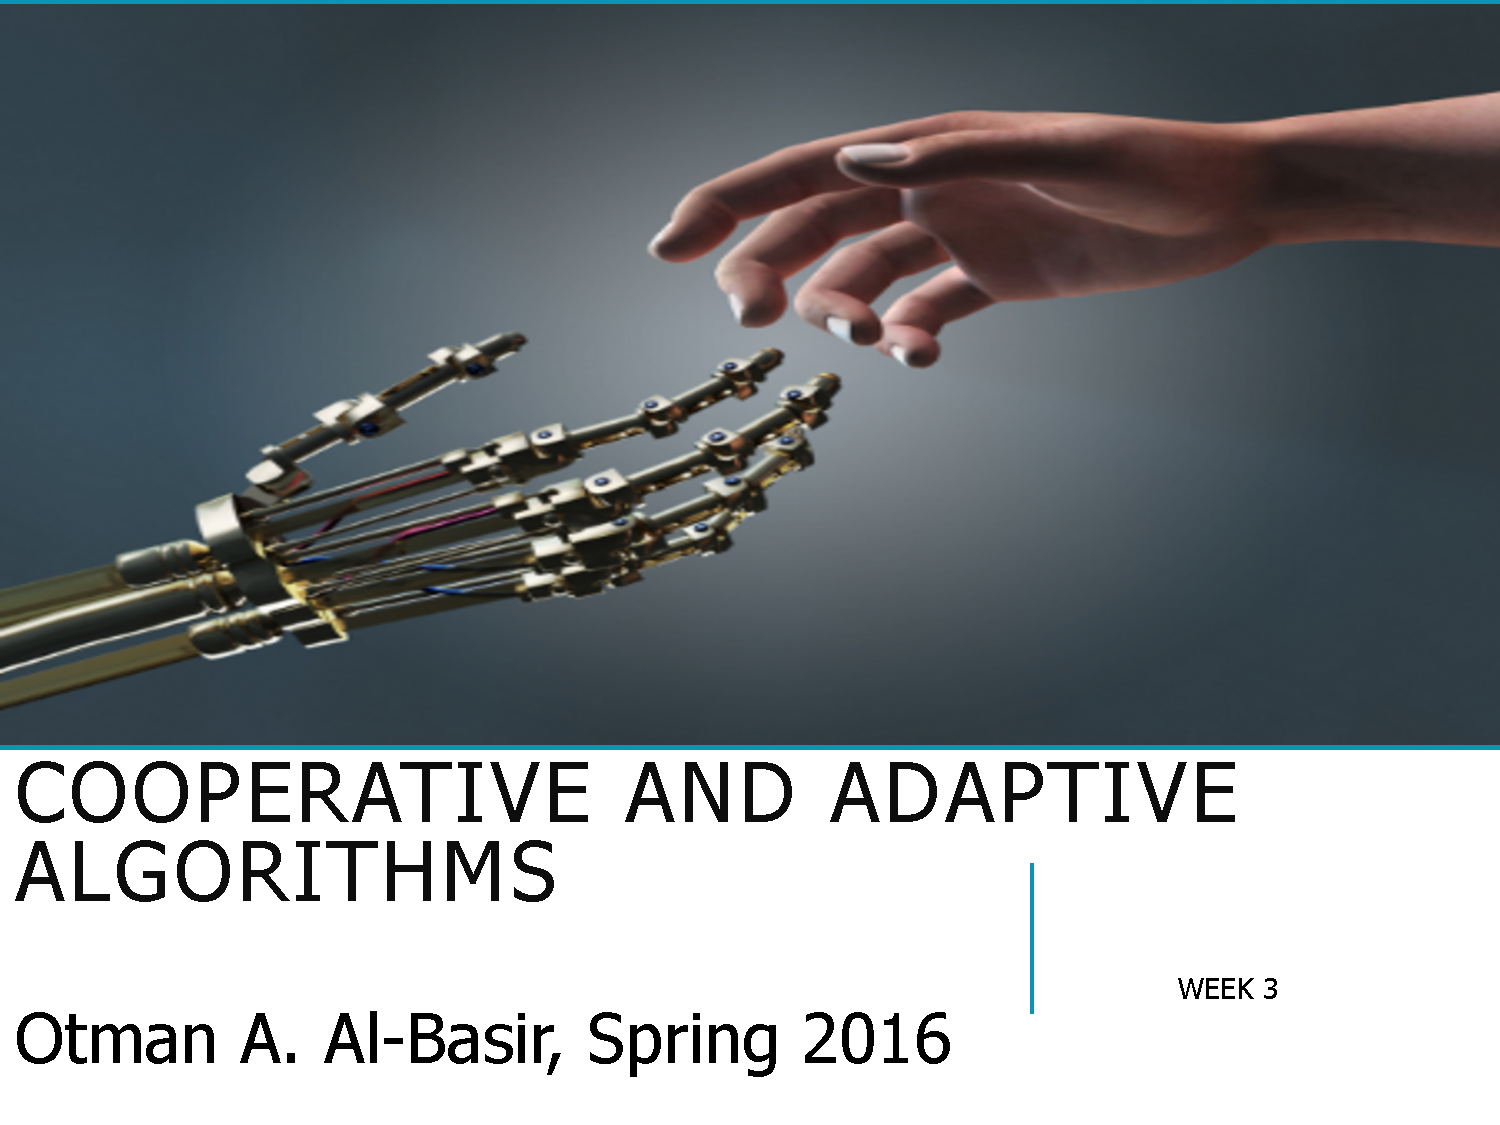
\includepdf[page=43]{slides.pdf}
So the base pointer to 1 and the next sequence number to 1, if the next sequence number is out of range we throw an error. If not we send properly and start a timer. If a timeout occurs start resending all unacked packets. If we get a valid packet back we move the acked pointer and adjust timers accordingly (ie change the timer to the next oldest one if this was the oldest packet). If we receive an invalid ack then we just do nothing.

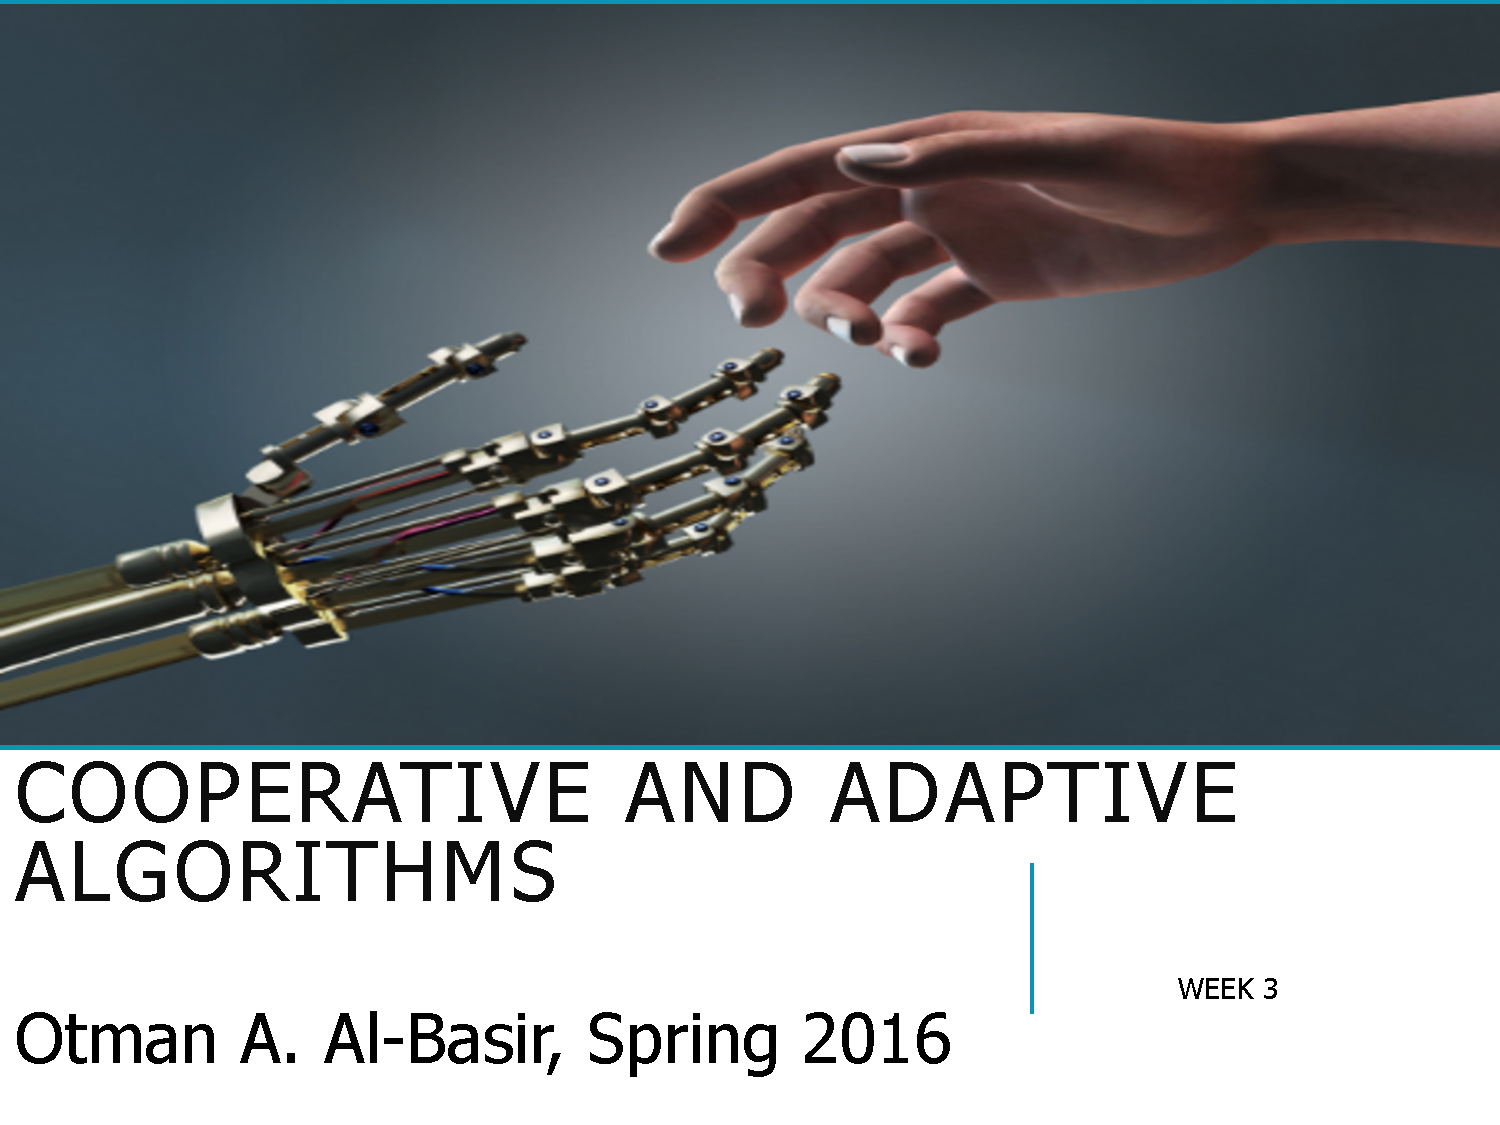
\includepdf[page=44]{slides.pdf}
There is a special exception on this. At the start of time you instantiate variables. If the first thing you receive is a corrupted packet you will acknowledge it. TCP doesn't do this since its number scheme is off by one, but here there is an error. 

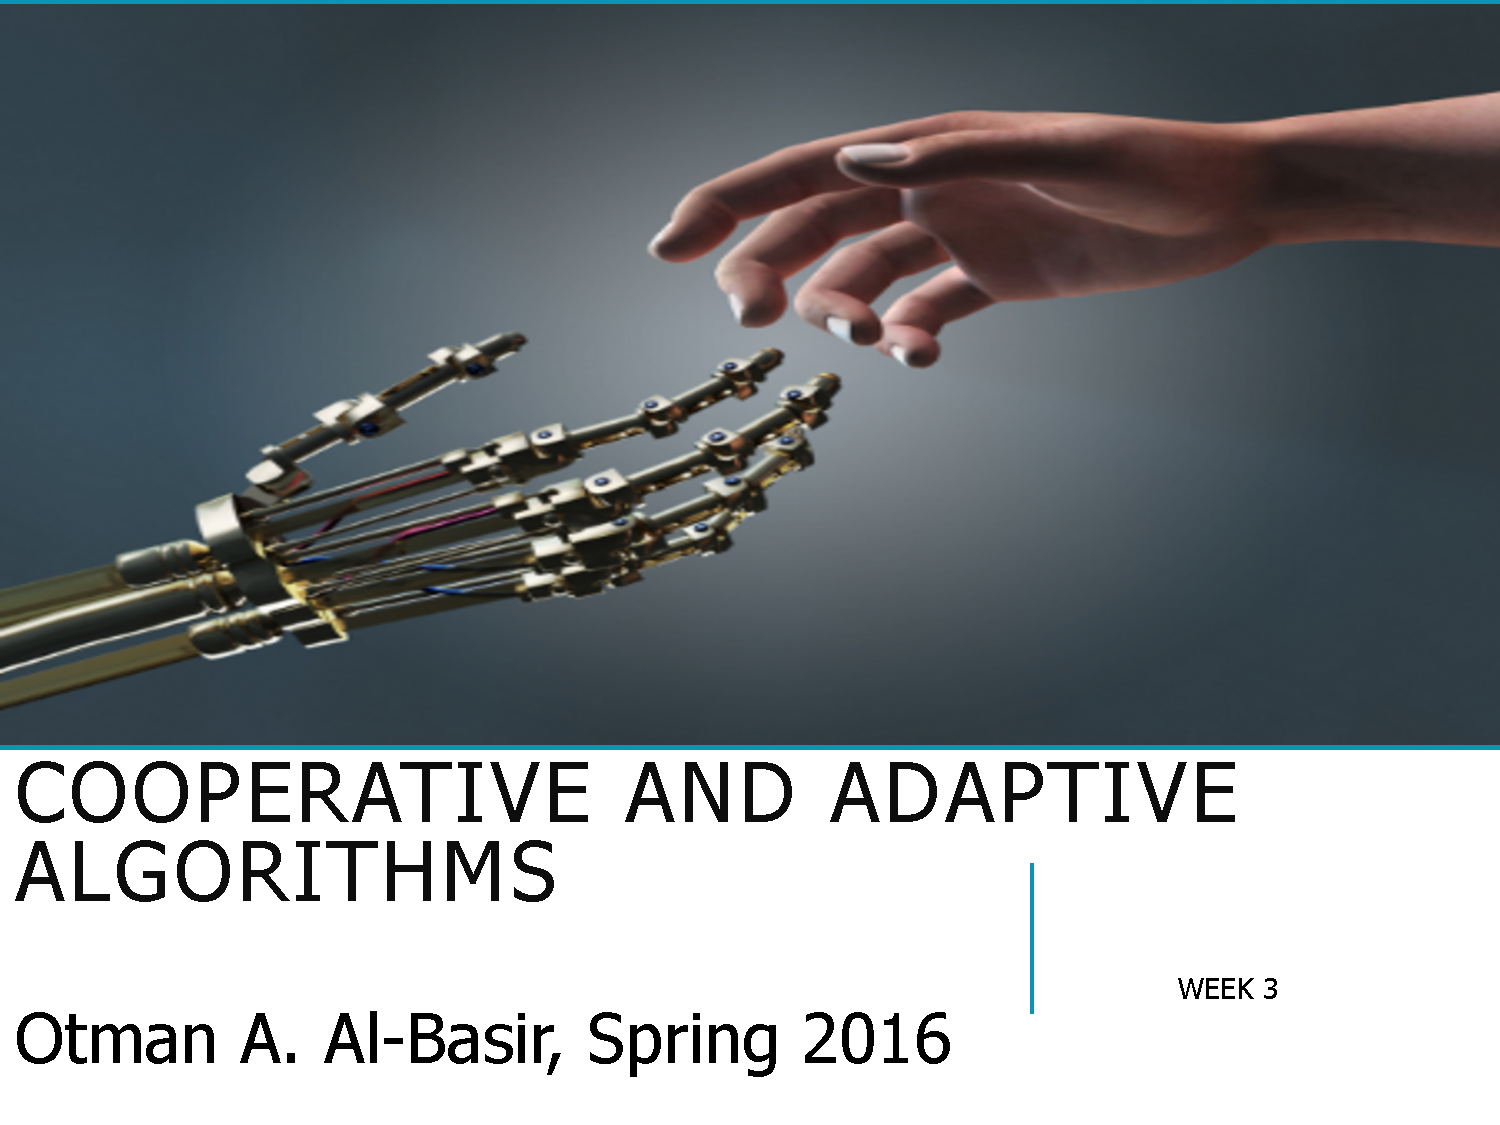
\includepdf[page=45]{slides.pdf}
When the sender receives ACK0 it shifts its base pointer and sends the next packet it can. We see in this example things ignoring duplicate acks, but in the psuedo code on slide we see it resets its based to that ack number plus 1. This is fine because it will just be set to the same number so its the same as doing nothing (it does however reset the timer which is an error). Every time we move the base we have to restart the timer. It becomes associated with the oldest unacknowledged packet.

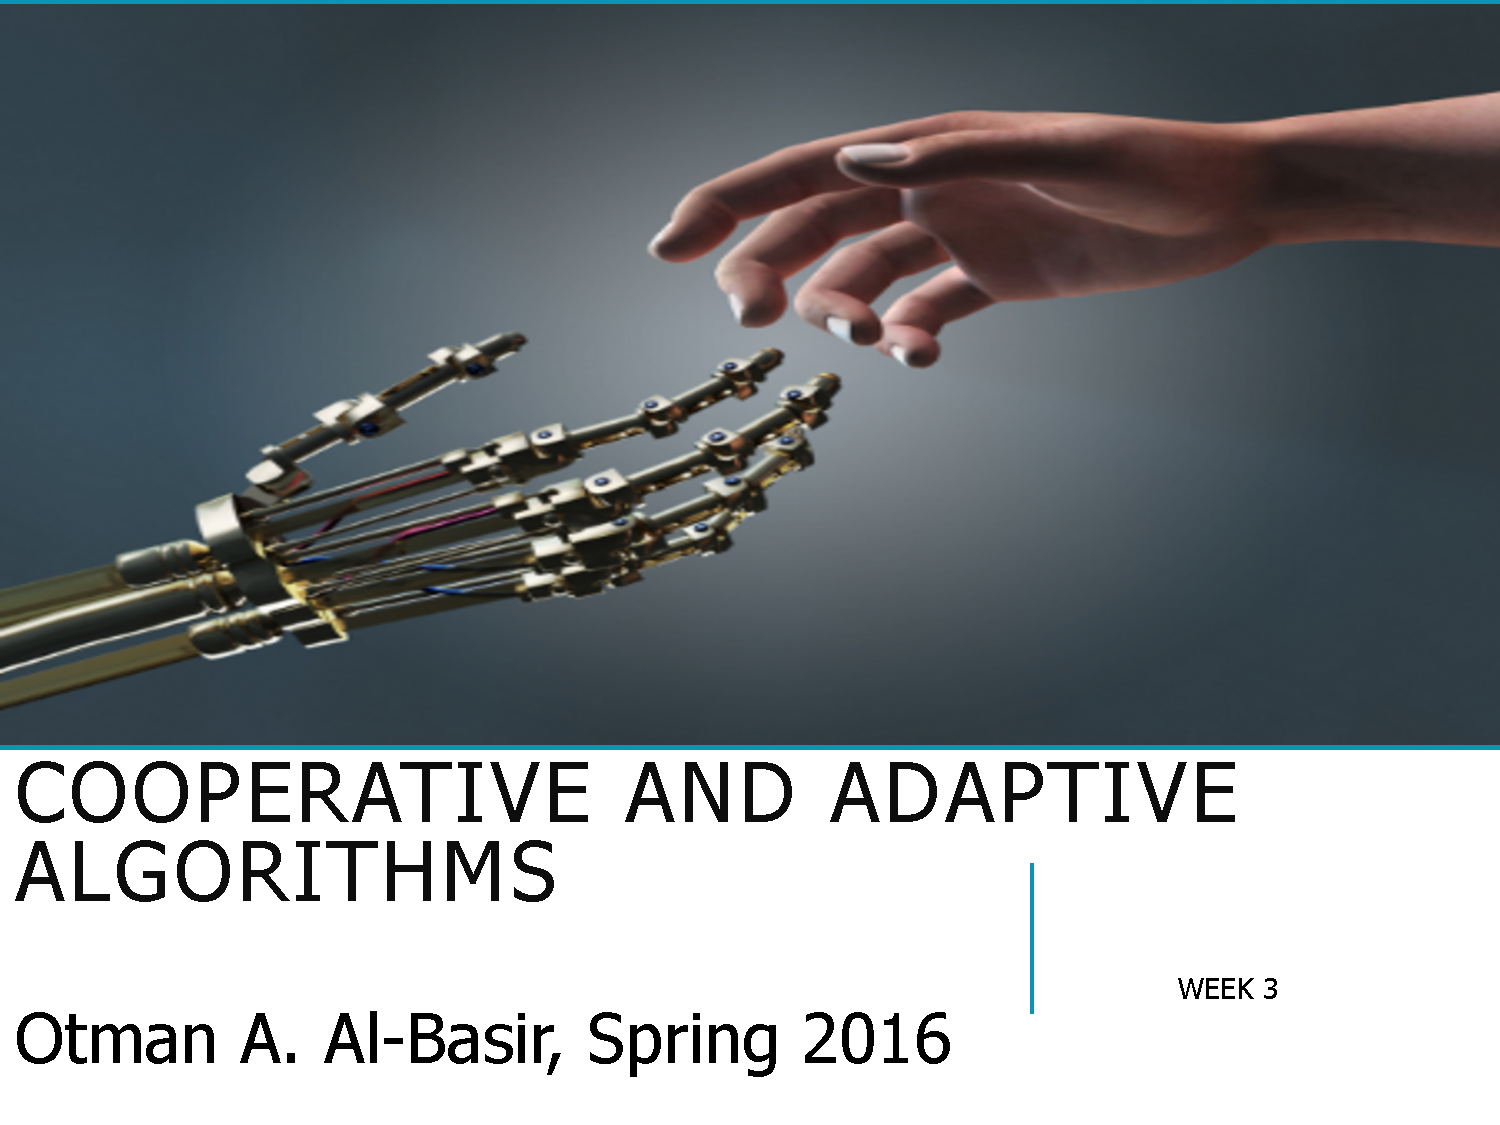
\includepdf[page=46]{slides.pdf}
Shit gets complicated here because the receiver acks individual packets so we need multiple windows.

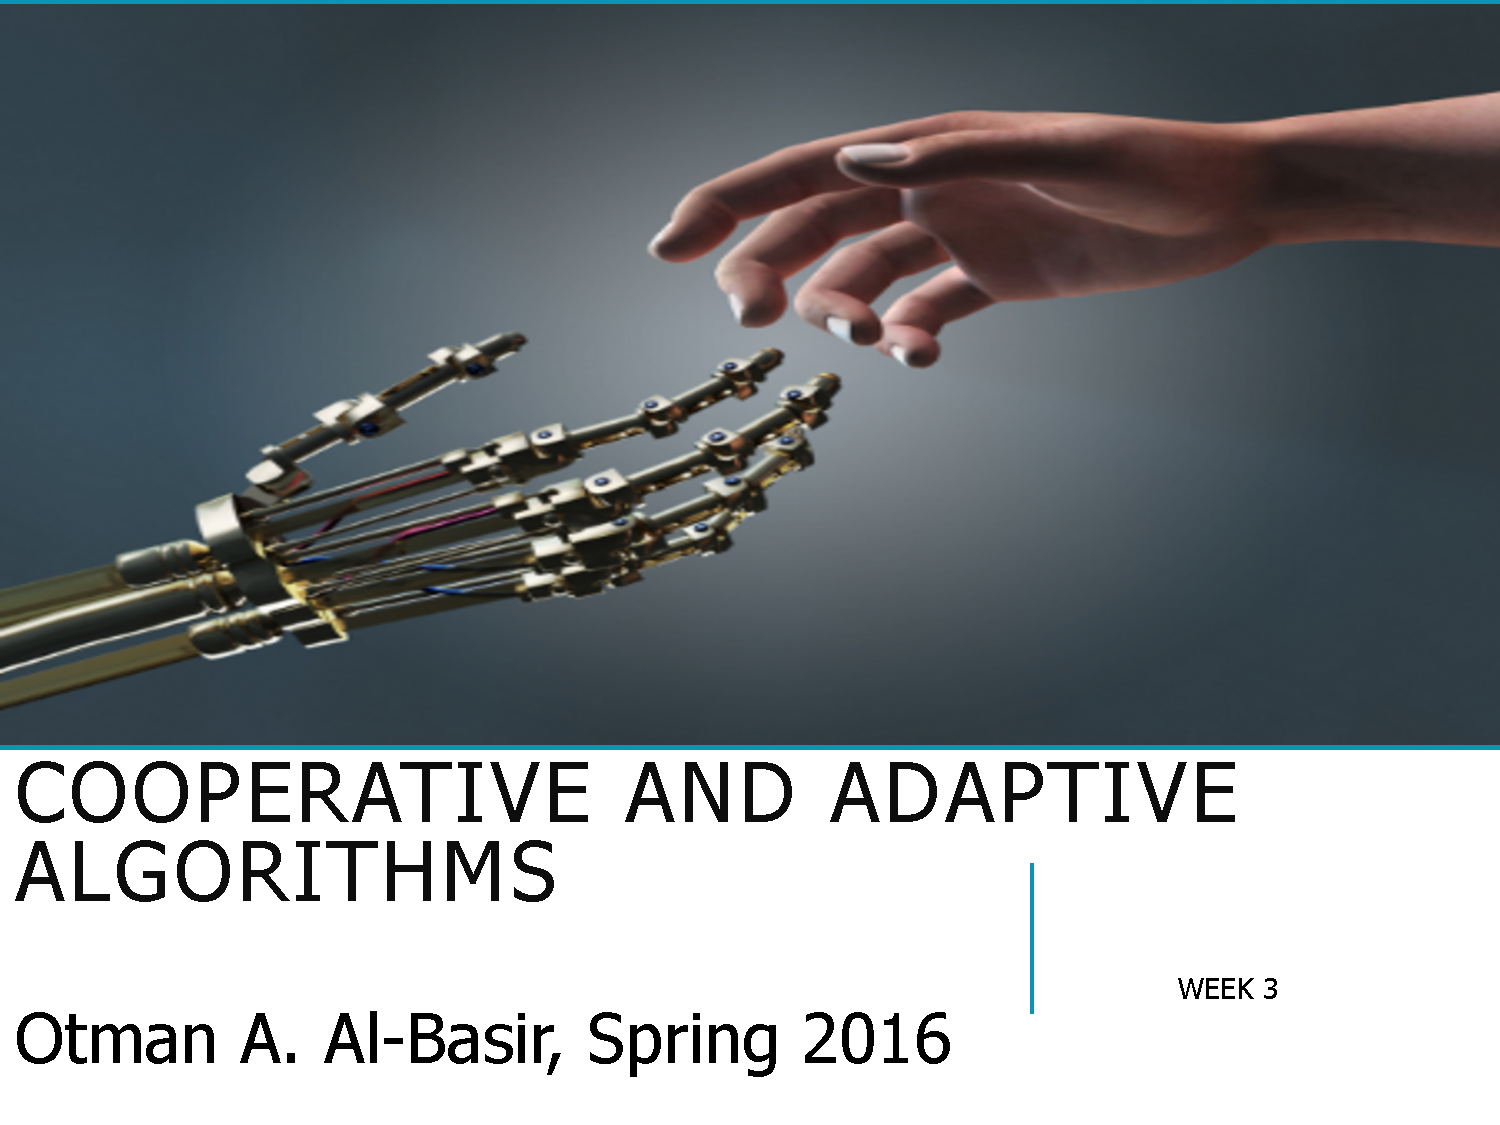
\includepdf[page=47]{slides.pdf}
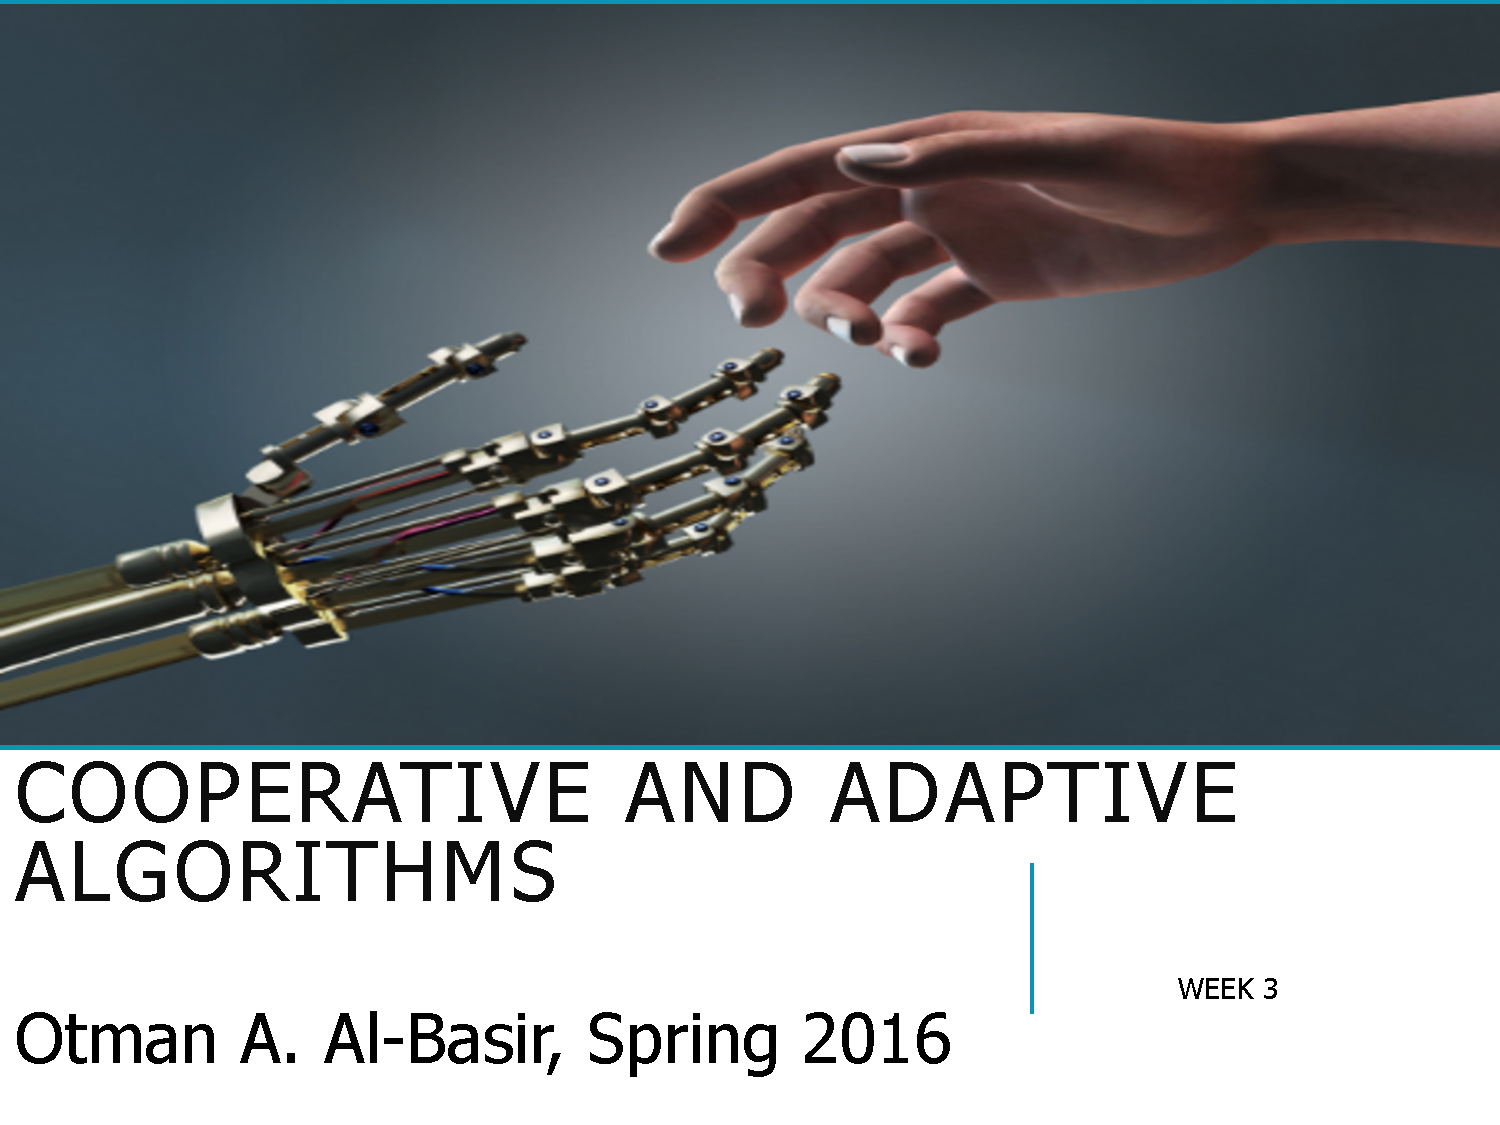
\includepdf[page=48]{slides.pdf}
We have a timeout per packet. When we receive an ACK we check that it is in out window (another error here, don't check the full window up to N, just up to the next sequence). When we move the base pointer we jump it to the next unacked packet (it jumps over all the previously acked packets that are consecutive).

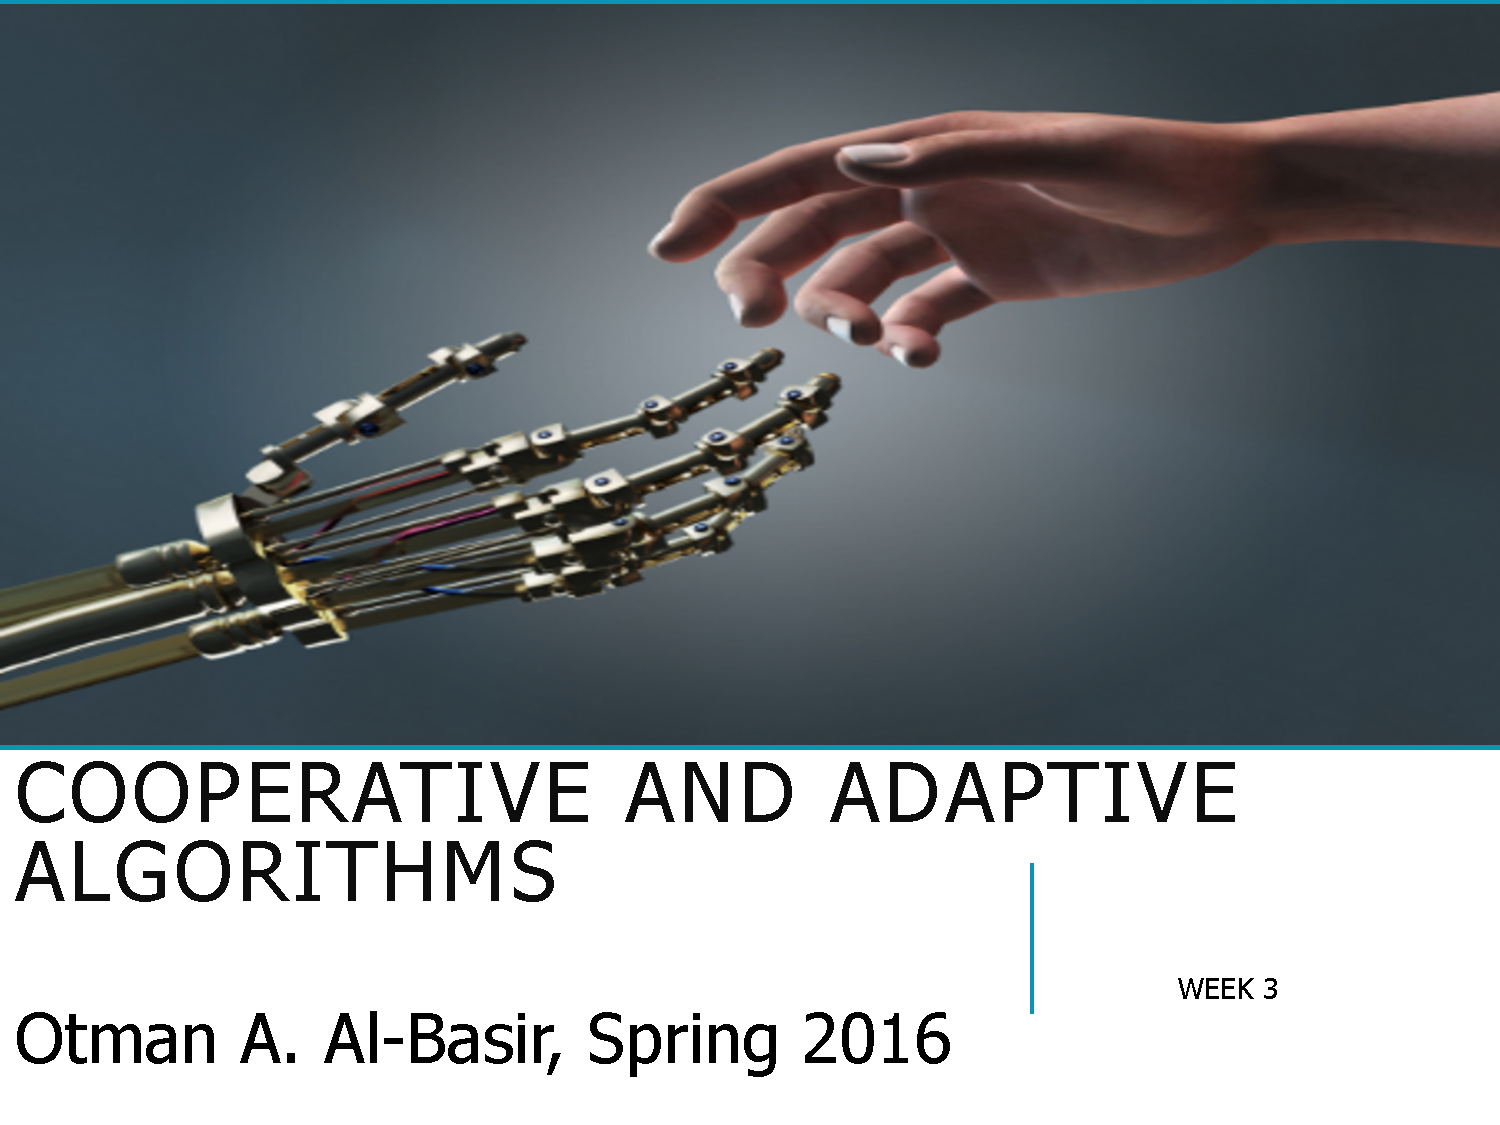
\includepdf[page=49]{slides.pdf}
When ACK2 arrives we advance the base all the way to 6.

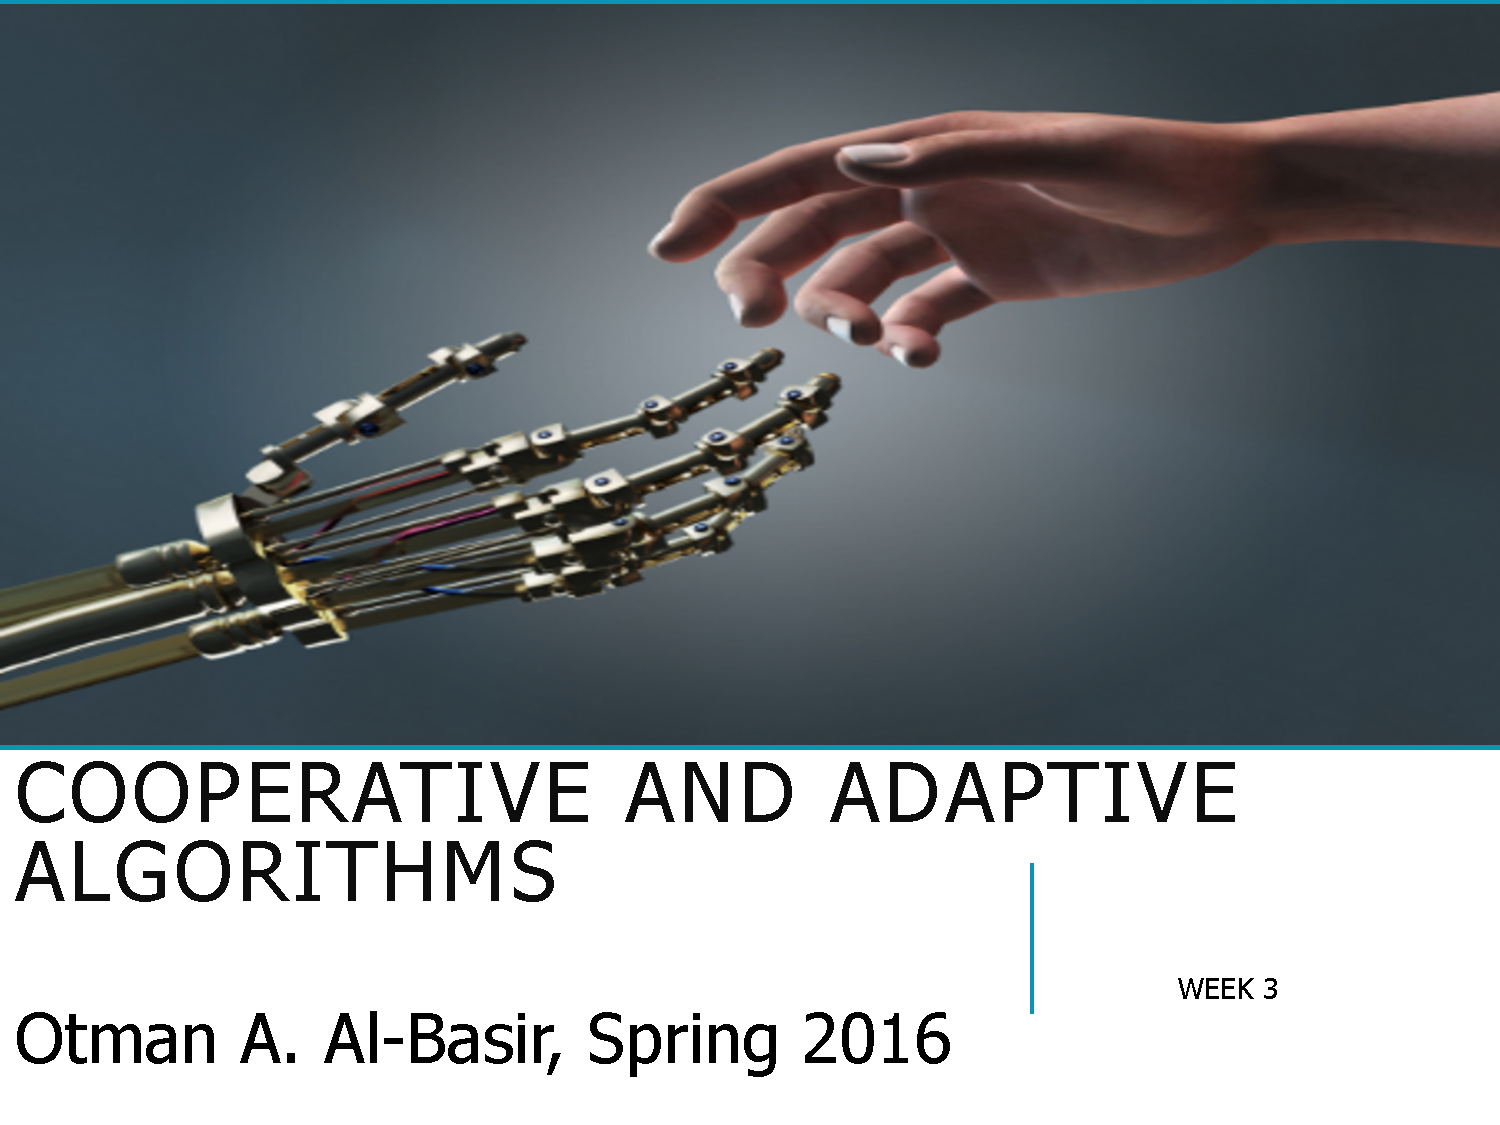
\includepdf[page=50]{slides.pdf}
From the receiver side it cannot distinguish between the two scenarios. The problem is that in the first scenario the second packet 0 is new content, but in the second scenario it is repeated data so its still old data, The receiver treats the second packet 0 as new content in both cases. This is wrong.


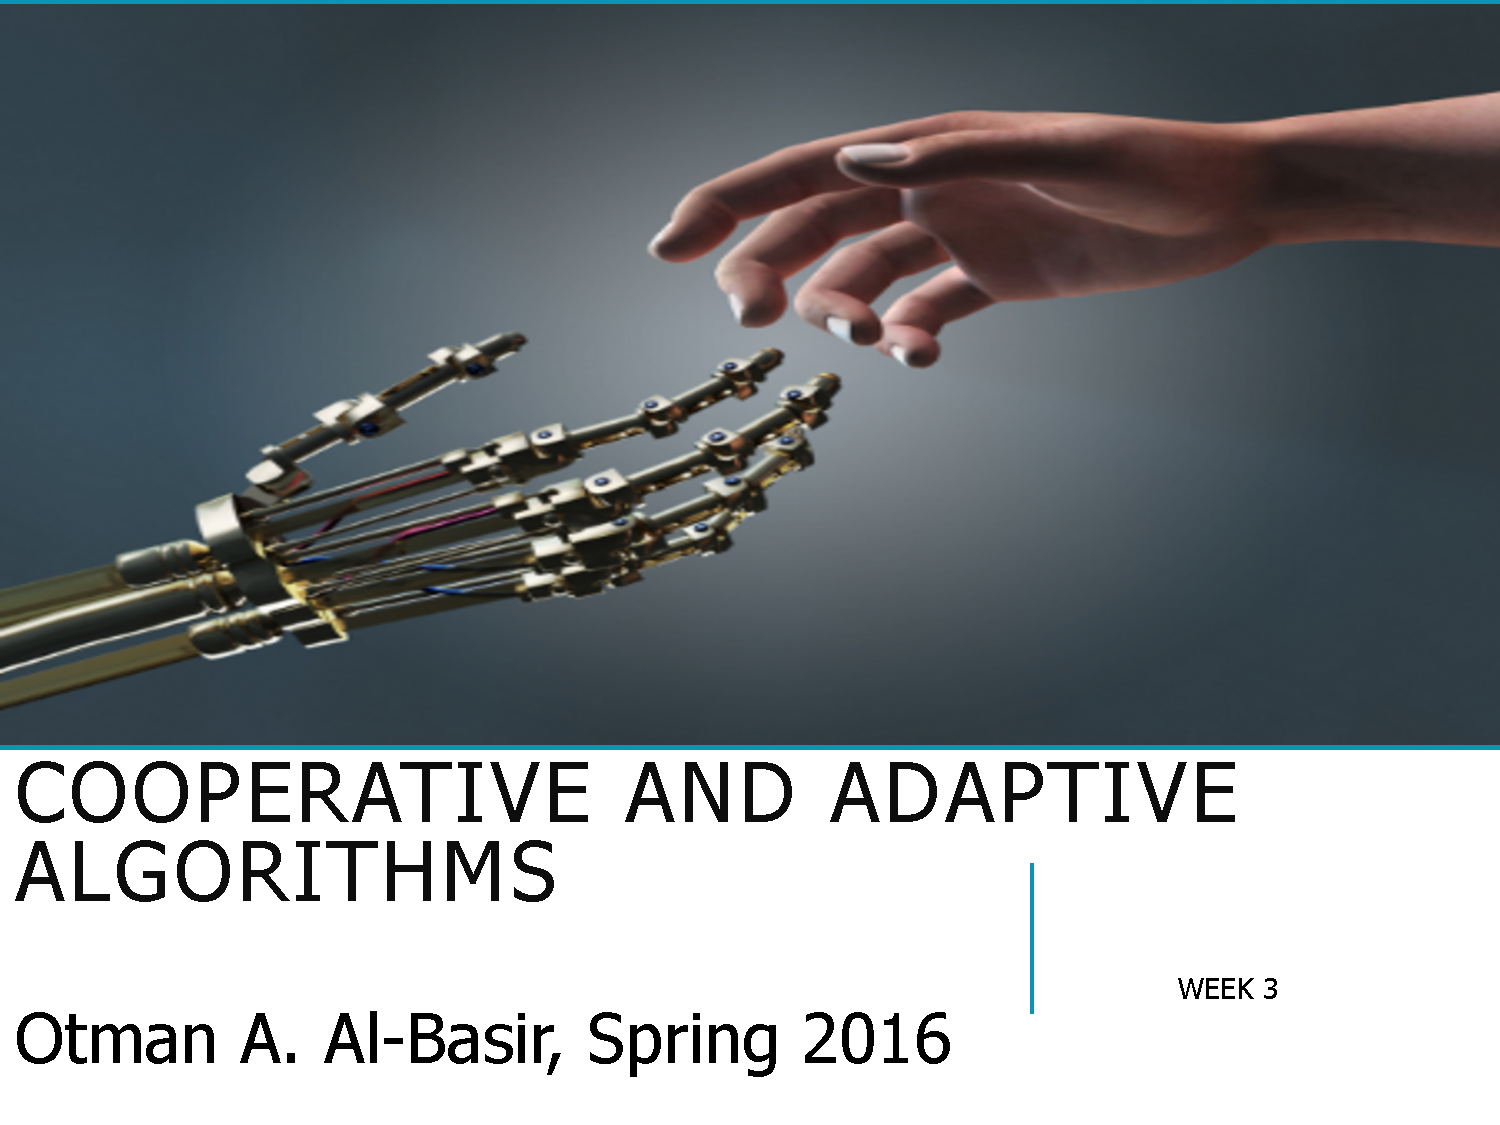
\includepdf[page=52]{slides.pdf}
There are no message boundaries. So when an application opens a TCP connection we don't need to know how much data we want to send. We can leave the connection open forever and send different sized chunks of data, It incorperates elements of selective repeat but its window is dynamic using congesting controls (will cover later). 

The application thinks that things are just byte streams, but TCP is actually packing them into segments and sending them. 

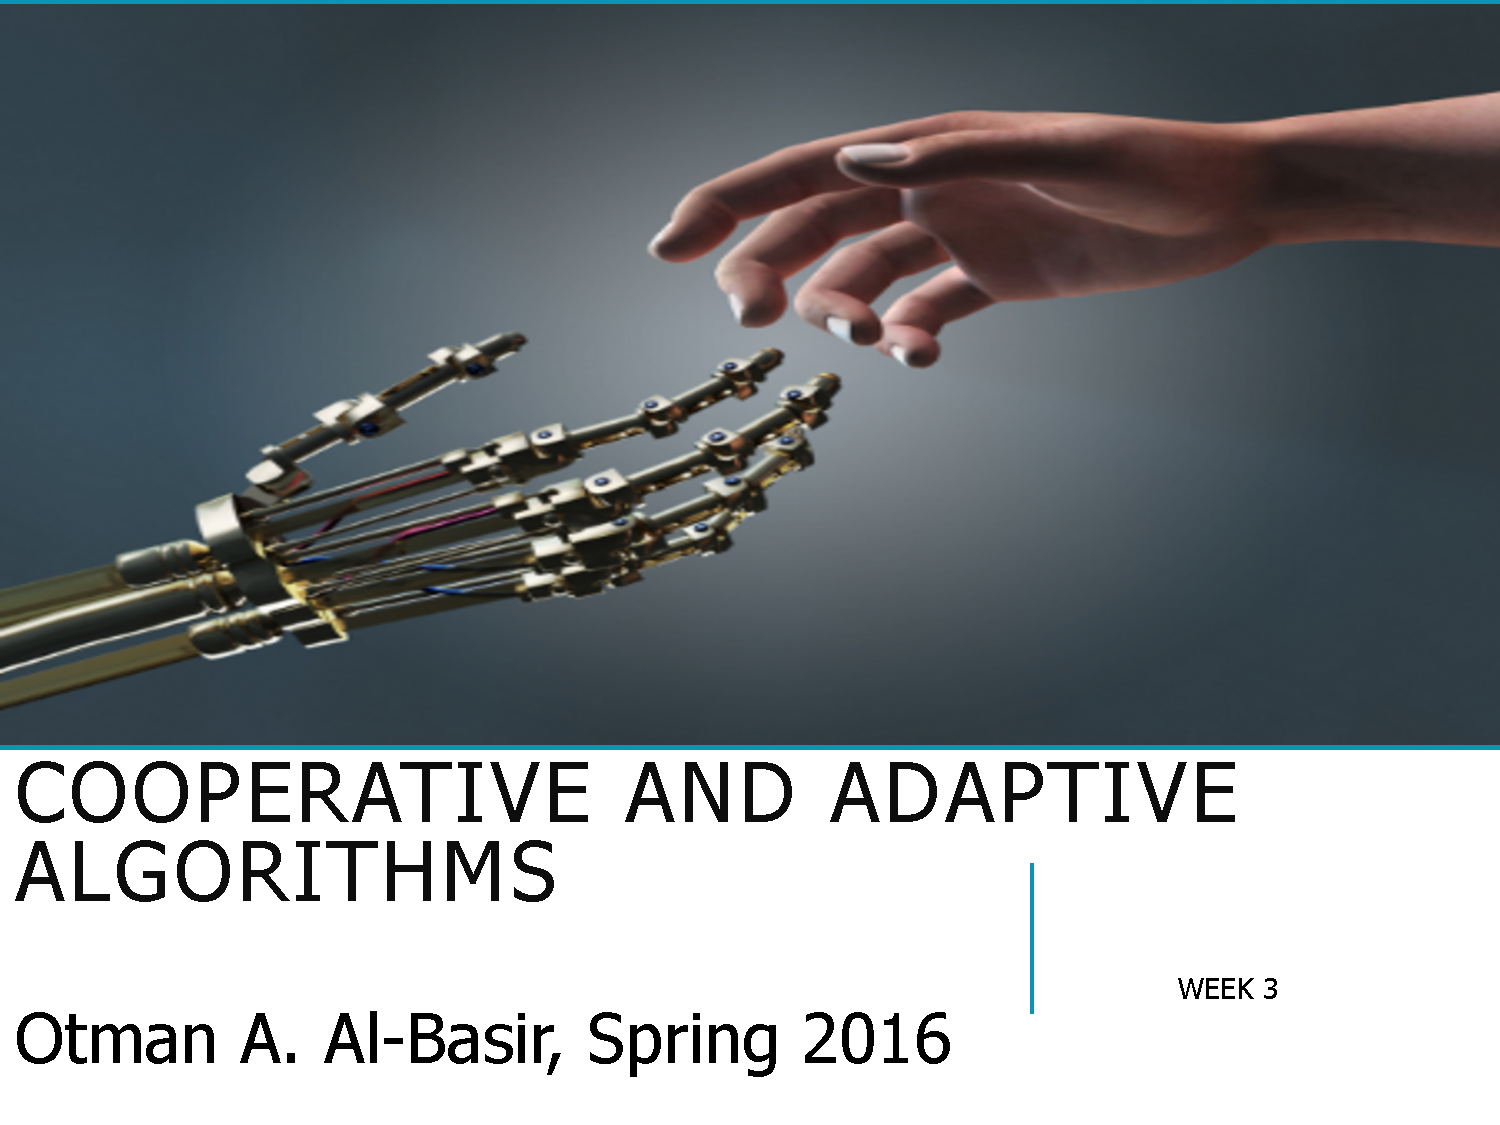
\includepdf[page=53]{slides.pdf}
The idea for the urgent flag is to say that this data is out of order, don't try to process it into your queue and such and just punt it to the application immediately. The ACK flag just says if you should pay attention to the ACK field (basically it might be garbage). The push flag works fairly similar to the urgent flag, but it doesn't do stuff if its out of order. The receive window is how big the receiver buffer is to prevent it from being overflown.

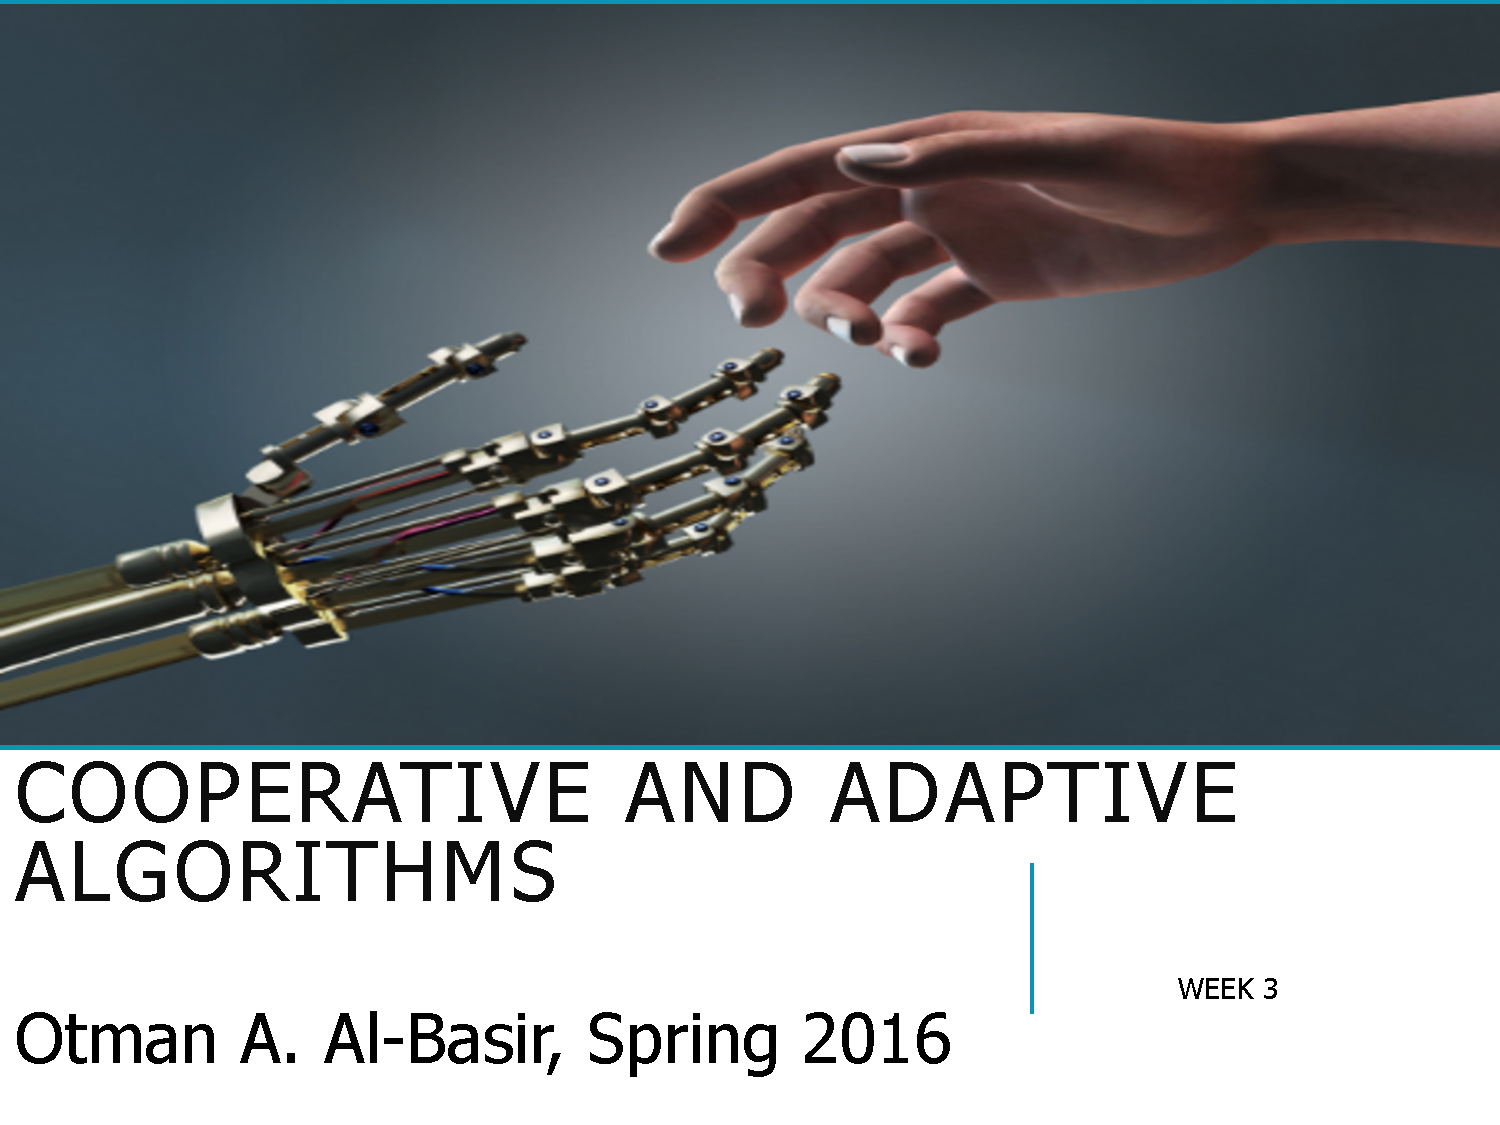
\includepdf[page=54]{slides.pdf}
The sequence number is actually the sequence number of the first byte of data and the acknowledgement is the ack of the next sequence number to be sent. So if we send a segment of size 50 it will have sequence numbers of 100-149 and its ack will be 150. There is very little standardization for how we handle out of order packets. Some places use selective ack.

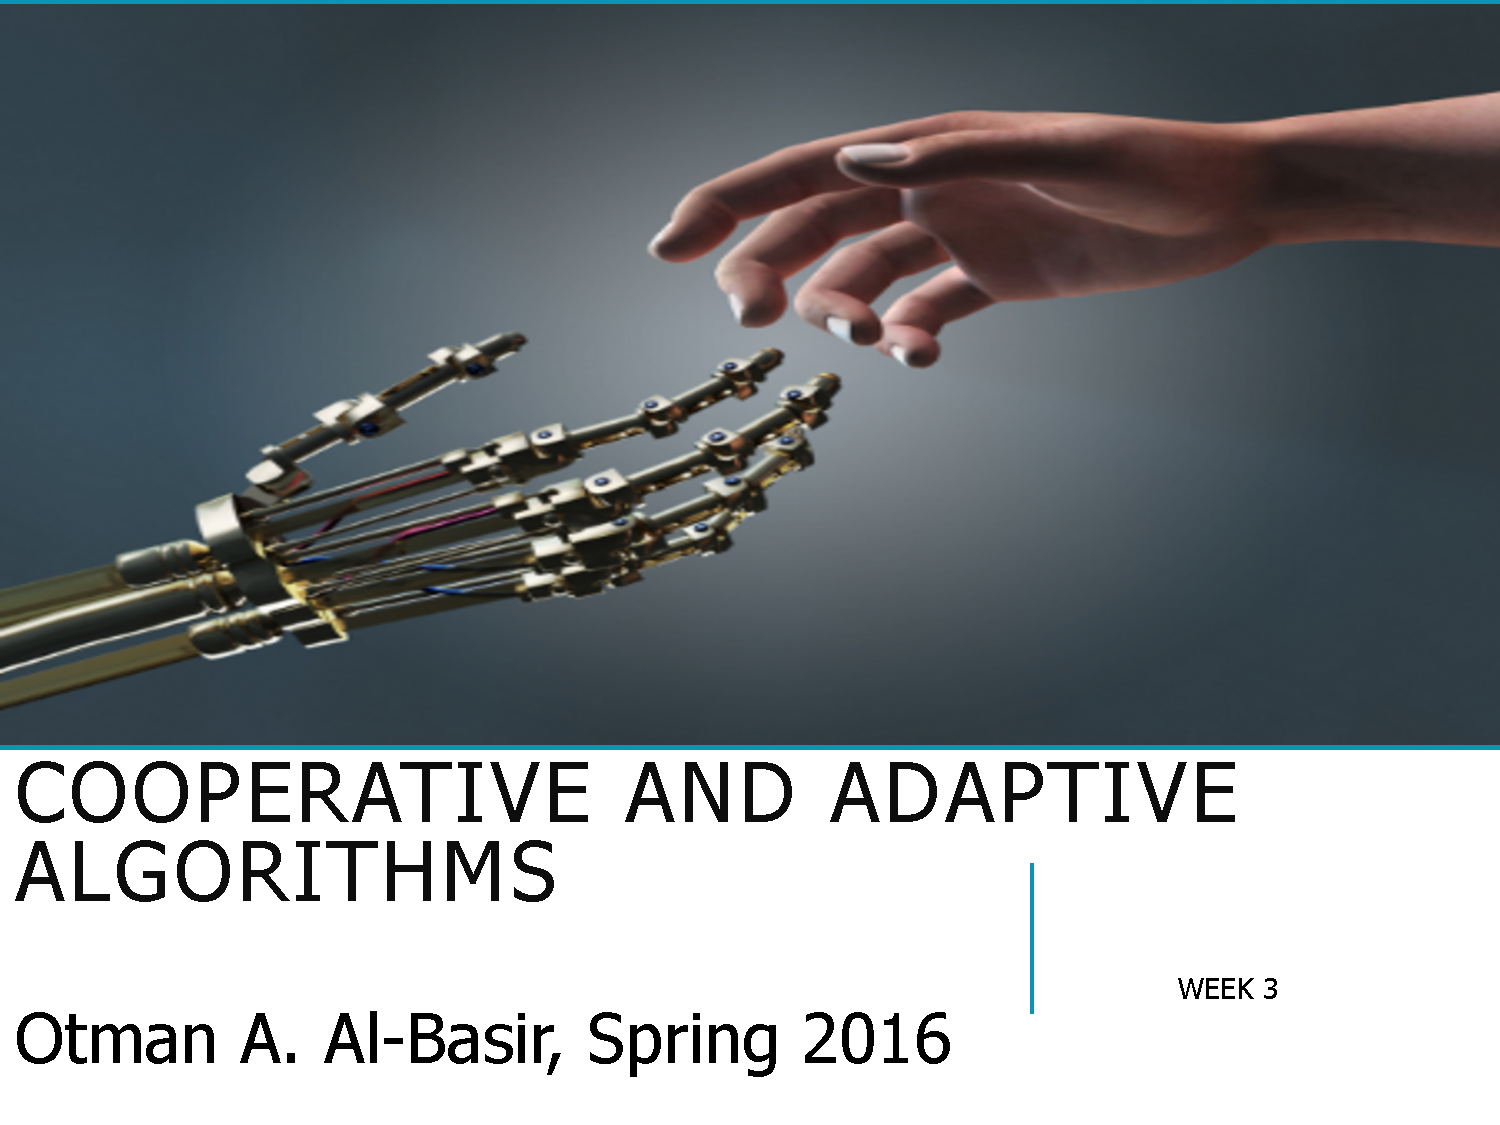
\includepdf[page=55]{slides.pdf}
Say we have a super boring echo server (just echos shit back to you).

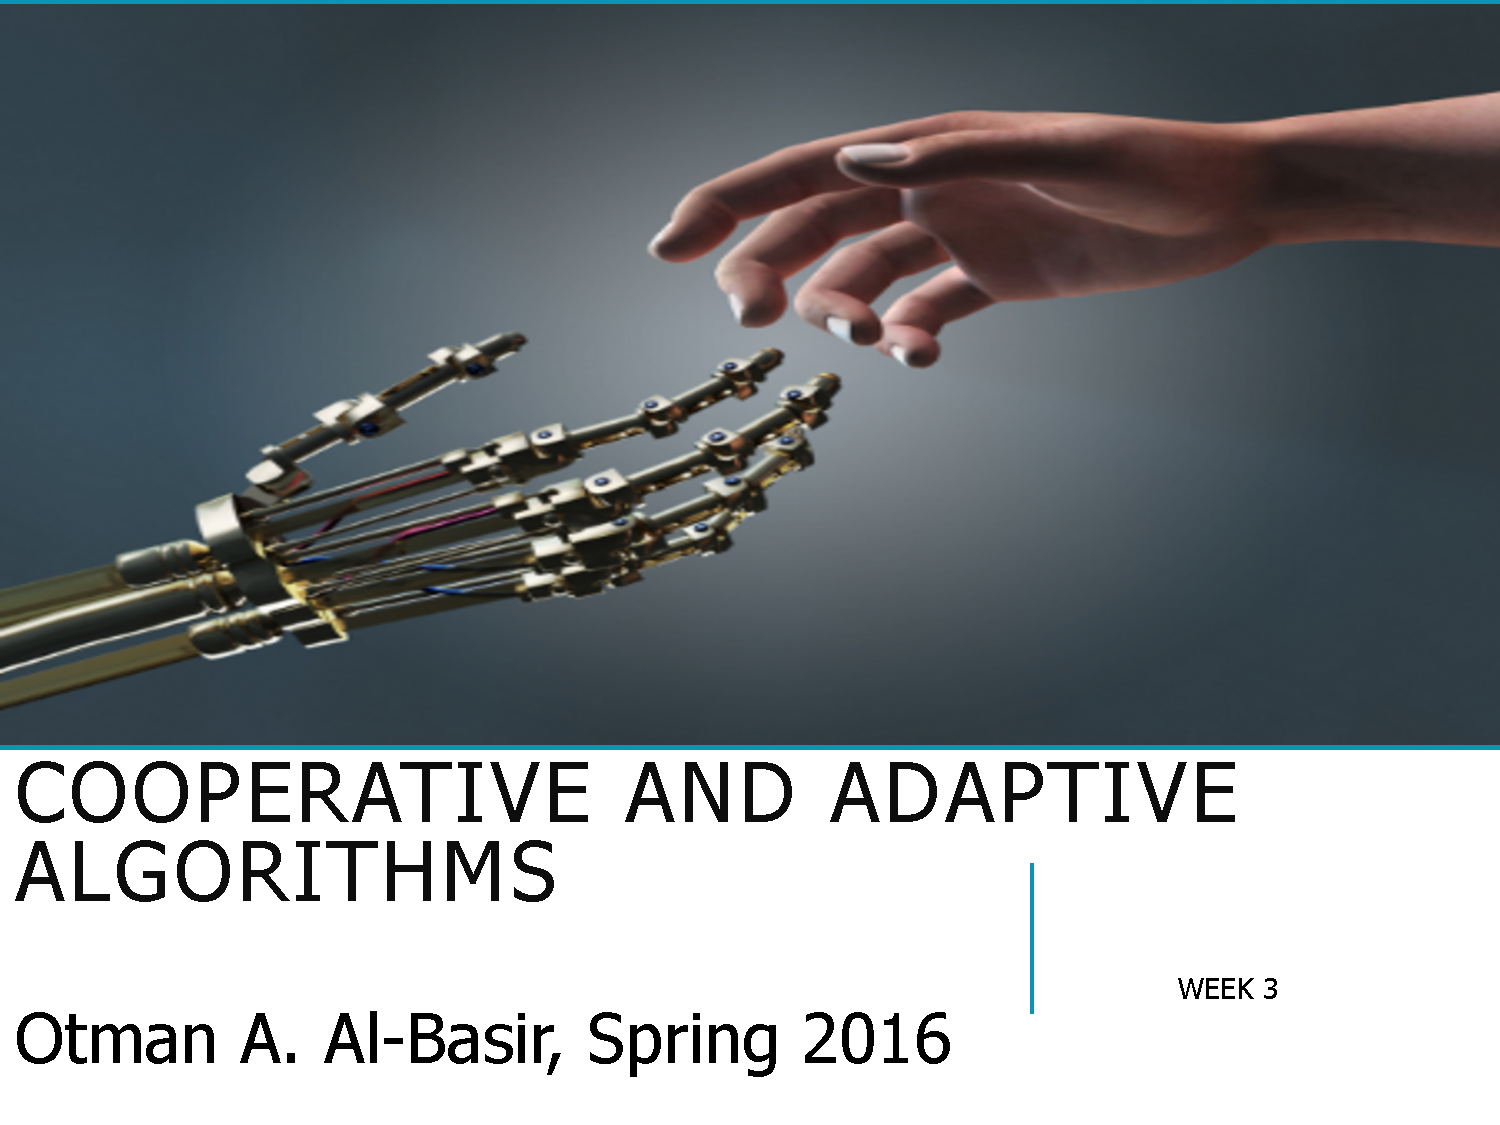
\includepdf[page=56]{slides.pdf}
Since TCP is a bit like go back n we need to handle timeout values. We want the timeout value to be something close to the round trip time so that we aren't waiting any longer than we have to but things still have enough time to get back. So TCP samples the roundtrip time and keeps updating its timeout values. The RTT is basically just sending a packet and timing how long it takes to get back (usually just a segment that was going to be sent anyway). This packet cannot be a retransmission because you might get the ack of the previously sent segment much faster than you should.


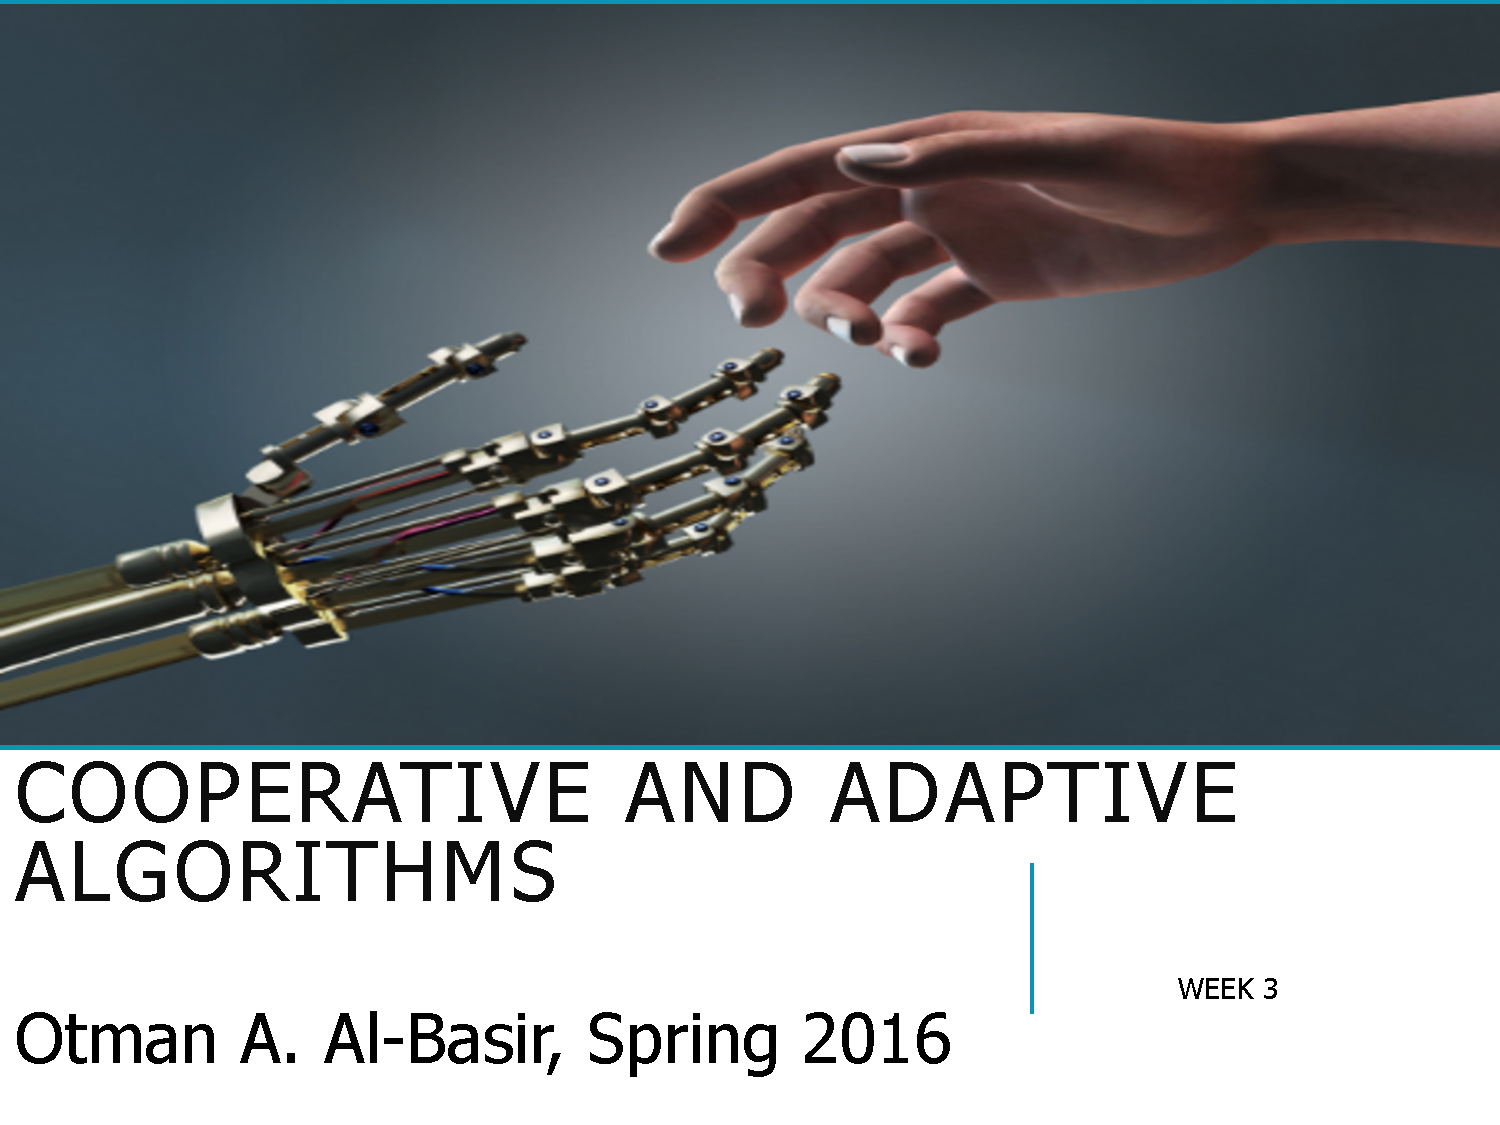
\includepdf[page=57]{slides.pdf}
We can apply an estimating formula to the sampled data you get back.

\includepdf[page=58]{slides.pdf}
We want to include a safety margin when calculating the estimated RTT. This safety margin wants to consider the previous variations so it looks at the historical deviation when calculating. This is so that what we sent our timeout too isn't so small is ignores all outliers. The 4 is basically a magic number. 

\includepdf[page=60]{slides.pdf}
The reliability of TCP is basically due to its incorperation of go back n. When TCP receives duplicate acks it infers some stuff before resending which is how it incorperates elements of selective repeat.

\includepdf[page=61]{slides.pdf}
The only part that is different from go back n is when a duplicate ack is received. We deal with checking for stale data.

\includepdf[page=62]{slides.pdf}
TCP is fairly high level so it can make some optimization assumptions. The ack is cummulative so were don't have to check for gaps. This should look surprisingly like go back n.

\includepdf[page=63]{slides.pdf}
If the sender sends two segments that timeout before either gets back we only resend the first one optimistically (we hope that only the first one was lost). We can change this protocol to resend all of them, but we dont watn to do that.

\includepdf[page=64]{slides.pdf}
The receiver also does some hoping when it receives so it delays a little bit hoping for more packets before it acks so that its ack can cover more.

\includepdf[page=65]{slides.pdf}
\includepdf[page=66]{slides.pdf}
If the sender receives duplicate acks for the same data, then it does a retransmit without a timer.

\includepdf[page=67]{slides.pdf}

\includepdf[page=69]{slides.pdf}
Devices on our network have different "power" levels.

\includepdf[page=70]{slides.pdf}
You want to buffer these packets to mitigate loss from one of your devices being much smaller than the other. We can use the network pipeline as a buffer and just at that to your receive window value. 

\includepdf[page=72-75]{slides.pdf}
when the receiver receives a syn they can respond with an ack and a syn of their own. This way the handshake is symmetric and gets around issues. 

\includepdf[page=76]{slides.pdf}
\includepdf[page=77]{slides.pdf}
\includepdf[page=78]{slides.pdf}
\includepdf[page=79]{slides.pdf}
Closing in a 4 way handshake. We send a fin packet and wait for a response. When the other side is ready (finished sending its shit). And so on.

\includepdf[page=81-105]{slides.pdf}


















\end{document}

%question about udp port numbers
%error on state diagram